\documentclass[12pt]{article}

\title{Building 3D Dense Reconstructions using LiDAR from a Walking Robot}
\author{Marcelo Gennari do Nascimento \\ Wadham College, University of Oxford}
\date{\today}

\usepackage{geometry}
 \geometry{
 a4paper,
 left=25mm,
 right=25mm,
 bottom=25mm,
 top=25mm,
 }
 
\setlength{\headheight}{14pt}
\setlength{\parindent}{4em}
\setlength{\parskip}{1em}
\usepackage{indentfirst}
\usepackage{setspace}
\usepackage{graphicx}
\usepackage{grffile}
\usepackage{sidecap}
\usepackage{svg}
\usepackage{enumitem}
\usepackage{wrapfig}
\usepackage{subfig}

\usepackage[labelfont=bf]{caption}
\usepackage{amsmath}
\graphicspath{ {images/}}
\doublespacing
\large

\begin{document}
	\pagenumbering{gobble}

	\maketitle

	\newpage

	\begin{abstract}
		Autonomous mobile robots depend on three connected fields of Robotics: perception, planning and control. The perception problem tries to answer where the robot is in relation to its surroundings, and it is a crucial step in planning and control.
		In recent years, many algorithms have been developed that solve very specific perception problems, although loosely related to each other. Some of these algorithms include Visual Odometry, Laser Odometry, Simultaneous Localization and Mapping, and 3D Reconstruction Systems.
		A full working autonomous mobile robot will have to integrate all of these algorithms and methods to work as expected even in challenging situations.
		The purpose of this project is to put together many of the modern algorithms in perception to evaluate how an integrated system performs with real-life data. The full system presented here consists of state-of-the-art algorithms in the fields aforementioned. The system is put to test using two different real-world datasets collected using the MultiSense SL sensor.
		It is hoped that this project will give rise to more integrated systems and an insight on the areas that need to be explored and further developed for a fully autonomous system.
	\end{abstract}

	\newpage
	\tableofcontents

	\newpage
	\pagenumbering{arabic}

	\section{Introduction}

Autonomous robots are going to be one of the major achievements of science to the benefit of the public. Autonomy though depends on two main problems that are closely related to each other: Localization and Mapping. The first concerns the problem of estimating the robot's position in an environment given a map as a prior. The second concerns the problem of mapping the environment given a prior robot's trajectory. Most of the time though, neither the trajectory nor the map is known \textit{a priori}, and they need to be built simultaneously. 

This is done by integrating a variety of sensors that can be categorized into proprioceptive or exteroceptive. Proprioceptive sensors provide data information about the robot itself, such as the forces in their joints and wheel encoders. Exteroceptive sensors give data information about the environment, using visual or laser scans for example. This is also called ``observations".
	
Since the 1986 IEEE Robotics and Automation Conference, researchers have framed the general problem of Simultaneous Localization and Mapping (SLAM) as the ``holy grail" of modern robotics \cite{SLAMPartI}. A reliable solution to this problem would make autonomy one step closer to reality. Since the conference, a number of algorithms have been developed that successfully tackle SLAM, each with their advantages and drawbacks. By integrating proprioceptive (inertial and kinematic) and exteroceptive (i.e. LiDAR) sensors, modern methods of localization are able to predict the position of a walking robot to within 2cm \cite{7041346}.
	
In order to make the map built have significant meaning and be of use to people, it is necessary to reconstruct it in 3D (or volumetrically). A 3D reconstruction system would give geometric, semantic and graphical meaning to maps, which then can be used for augmented or virtual reality for exampled.
	
Volumetric reconstruction relies heavily on tracking the robot's position, since the observation accuracy is independent from other observations but bounded by the tracking accuracy. Therefore, by using modern techniques to solve the problem of SLAM, it would be possible to build a reliable and realistic map of an environment without any prior information about how the environment is structured. Obvious direct applications for such a system would be reconnaissance, search and rescue, and transportation.
	
	\subsection{Aim of the Project}

This project is concerned about putting together state-of-the-art algorithms for SLAM and reconstruction systems to reliably and efficiently build a 3D map of an environment with LiDAR data from a walking robot without any prior map or trajectory available. Since the robot is most likely to operate indoors and in situations where no off board sensor is available, it was decided to not use any wirelessly transmitted information, such as GPS (Global Positioning System) or Motion Capture Systems.
	
Many papers have been published on the individual building blocks that form the components of this project, whereas academic reports that put all of the state-of-the-art algorithms together to form a working system are much rarer. This report is the result of such a system. The contributions of this report are: (1) The design of a SLAM and 3D Reconstruction system integrating modern algorithms; (2) Validation of the system in real-data collected using a LiDAR sensor.
	
	\subsection{ Organisation of the Report}

\paragraph{Section 2} of the report will go through the literature review of the main building blocks of the project. In particular, current developments in the solutions of the Simultaneous Localization and Mapping (SLAM), Stereo Visual Odometry, the Iterative Closest Points (ICP), and 3D Reconstruction problem.
	
\paragraph{Section 3} will go deeper on the system pipeline of the project. In order to get a general understanding of the system, detailed explanation of the steps of data processing, inputting and outputting will be explained. This will also introduce the two main parts of the system that will be explained in subsequent sections and analyse the tools used in the project.
		
\paragraph{Section 4} explores the solution of the SLAM problem adopted in the project. Since building an accurate map is an essential step to the success of the project, this section will explain the details of how the SLAM solution works and why this particular structure was chosen.
		
\paragraph{Section 5} shows how the output from the SLAM solution will be integrated with the 3D reconstruction system. This has been a major topic of research in Computer Vision and Computer Graphics, but have mainly been tackled in small environments and in hand-held devices. In this section, a solution for large scale reconstruction, and an overview of the parameters and trade-off involved in the process will be explored.
		
\paragraph{Section 6} presents the results on real-data, collected using LiDAR sensors. In this section, the software and hardware used to get the results, and a comparison between the results in the datasets will also be presented.
		
\paragraph{Section 7} will conclude the report with an overall evaluation of how the system performed. It will also indicate ways in which the system could be improved in a subsequent project. An analysis of how the outcome of this project compares with similar systems will be provided.

	\newpage
	\section{Literature Review}

	\subsection{Simultaneous Localization and Mapping (SLAM)}
	\label{subs:SLAMRev}

SLAM is the problem of whether it is possible for a mobile robot to create a globally consistent map of an environment and localize itself on it without prior knowledge of the map \cite{SLAMPartI}\cite{Cadena}. Building a map of an environment is a crucial step towards autonomy, since planning and control assume prior knowledge of mapping and localization. Mathematically, we can frame SLAM as a Bayes Net. Defining:
	
\begin{itemize}
\item $\mathbf{x_k}$: the pose of the robot (being $\mathbf{X_{0:k}}$ as the poses from time $\mathbf{0}$ to $\mathbf{k}$)
\item $\mathbf{u_k}$: the odometry measurement ($\mathbf{U_{0:k}}$ as the historical measurements)
\item $\mathbf{l_k}$: the landmark position ($\mathbf{L_{0:k}}$ as the historical landmarks)
\item $\mathbf{z_k}$: the landmark observation ($\mathbf{Z_{0:k}}$ as the historical landmarks)
\item $\mathbf{c_k}$: the loop closures
\end{itemize}

It is possible to formulate the problem of SLAM more formally using the following graphical model:

\begin{SCfigure}[][ht!]
\begin{minipage}{0.65\textwidth}
\centering
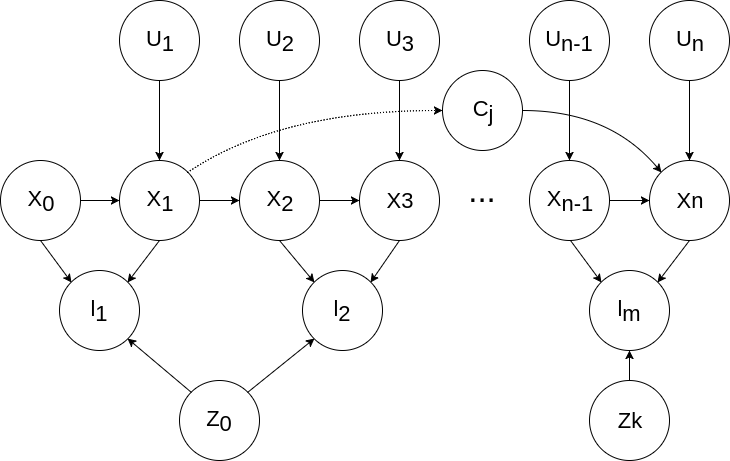
\includegraphics[width=\textwidth]{BayesNetSLAM}
\end{minipage} \hfill
\begin{minipage}{0.35\textwidth}
\centering
\caption{SLAM as a Bayes Net. The value $\mathbf{x_0}$ denotes a prior; $\mathbf{x_n}$ denotes the state vector; $\mathbf{u_n}$ denotes odometry measurements; $\mathbf{c}$ denotes close loops; $\mathbf{l_n}$ denotes landmark positions.}
\label{fig:slam1}
\end{minipage}				
\end{SCfigure}
	
The graph shown in Figure \ref{fig:slam1} is a Bayes Network representation of the dependencies between variables. A probabilistic framework can then be extracted from it. 

\begin{equation}
P(X,L,U,Z)\ \propto \ P(x_0)\prod_{j=1}^{M}P(x_j|x_{j-c},c_j)\prod_{i=1}^{M}P(x_i|x_{i-1}, u_i)\prod_{k=1}^{K}P(z_k|x_{i_k},l_{j_k})
\label{eq:probSLAM}
\end{equation}

The general goal of probabilistic SLAM is to find variables $\mathbf{X^*}$ and $\mathbf{L^*}$ that maximizes the posterior probability distribution $P(X,L\ |\ U, Z)$ of the Equation \ref{eq:probSLAM}. Two models of the probabilities given above are used commonly in SLAM to tackle this problem: the Process Model (also known as Motion Model in mobile robotics) and Observation Model:
	
\begin{minipage}{.48\linewidth}
\centering
\begin{equation*}
\begin{split}
\mathbf{Process\ Model:} \\ 
x_i = f(x_{i-1}, u_i) + w_i
\end{split}
\end{equation*}
\end{minipage}
\begin{minipage}{.48\linewidth}
\centering
\begin{equation*}
\begin{split}
\mathbf{Observation\ Model:} \\ 
z_i = h(x_{i_k}, l_{j_k}) + v_k
\end{split}
\end{equation*}
\end{minipage}
	
Where $w_i$ is white noise with covariance $Q$ and $v_k$ is white noise with covariance $R$. The process (motion) model is usually a generalization of how the robot moves (kinematics) \cite{Montemerlo02fastslam:a}\cite{772544}. The observation model is a probabilistic representation of the performance of the sensors used to collect the data. Notice that both models are probabilistic and thus define the probability distributions $p(x_i|x_{i-1},u_i)$ and $p(z_k|x_{i_k},l_{j_k})$.

Under this framework, it was shown that the SLAM problem is indeed feasible, and that it builds a nondivergent map with no prior information \cite{CsorbaThesis}. So it is widely accepted that in theoretical grounds, SLAM is a solved problem \cite{SLAMPartI}\cite{Cadena}\cite{CsorbaThesis}\cite{938381}. However, there are computational and algorithmic challenges that hinders the development of a real-time implementation system that performs SLAM. This problem gets even more complicated when considering unstructured environments and large scale maps \cite{SLAMPartII}.
	
There are three main implementations of SLAM: Kalman Filtering and Extended Kalman Filtering (with early works such as proposed by R. Smith \cite{Smith:1990:EUS:93002.93291}), Particle Filtering (most notably with FastSLAM \cite{Montemerlo02fastslam:a}) and Information Filter (with iSAM from Michael Kaess \cite{Kaess08tro}).

	\subsubsection{Kalman Filtering}

As one of the first implementations to attempt to solve the problem of SLAM, the Extended Kalman Filtering (EKF) approach makes two approximations when formulating the probabilistic SLAM: both the Process Model and the Observation Model are linearised about a suitable linearisation point $\hat{x}$.

 Subsequently, the probability distributions $p(x_i|x_{i-1}, u_i)$ and $p(z_i|x_i, l_i)$ are modelled as Gaussians with the means $\nabla f|_{x=\hat{x}}$ and $\nabla h|_{x=\hat{x}}$ and covariances $Q$ and $R$. With this framework in place, a recursive two-step method can be found to update the posterior probability distribution at every iteration \cite{SLAMPartI}:

\begin{equation*}
\mathbf{Prediction\ Phase:}\ \ 
P(x_{i},L|Z_{0:i-1}, U_{0:i}) = \int P(x_i | x_{i-1}, u_{i}) P(x_{i-1}, L |Z_{0:i-1}, U_{0:i-1})dx_{i-1}
\end{equation*}
\begin{equation*}
\mathbf{Update\ Phase:} \ \  P(x_i, L | Z, U) = \frac{P(x_{i}, L | Z_{i-1}, U)P(z_i|x_i,L)}{P(z_i|Z, U)}
\end{equation*}	 	

The Prediction Phase concerns the motion model, where an update of the estimated position of the mobile robot is made taking into account only the controls and kinematics of the robot itself. This is followed by an Update Phase, where the position of the robot is recalculated based on the observation of a landmark, for example. This algorithm is then recursively applied for every time-step $i$. 	

Since the product of two Gaussians is a Gaussian, the probability density function $p(x_i, L|Z, U)$ will remain Gaussian at all times, and a closed loop solution using just the mean and the covariance matrices can be found \cite{772544}.

Analysis of the EKF algorithms have shown that due to linearisation of the functions $f$ and $h$, assumptions about Gaussian Process and Observation Model can cause the EKF solution to perform poorly unless many loop closures are detected in frequent intervals \cite{doi:10.1177/1729881416669482}.

It is also known that the Kalman Filter approach requires storage of the order of $O(N^2)$ (where $N$ is the number of features), and for a classic implementation of the algorithm, it also requires computational power of the order of $O(N^2)$ \cite{CsorbaThesis}. New methods for computing the covariances (which cause the squared dependence) by exploring state augmentation, partitioned updates and sparsity in the matrices have demonstrated faster solutions, thus requiring less computational power \cite{SLAMPartII}.

	\subsubsection{Particle Filtering}

In order to avoid linearisation of non-linear models, Particle Filtering (PF) has been a popular method to integrate non-Gaussian distributions in the estimation \cite{Montemerlo02fastslam:a}\cite{772544}. The basis of particle filtering comes from Dallert's proposal of a Monte Carlo Localization (MCL) algorithm \cite{772544}. In sampling methods, the probability distributions are defined as a function of the density of particles along the distribution. This approach avoids the assumption of linearity and Gaussian distribution, which makes this algorithm embrace multi-modal distributions.
	
Just like the EKF solution, there are many different implementations of PF methods. However, most of them follow the basic structure of the FastSLAM algorithm \cite{Montemerlo02fastslam:a}. This algorithm breaks the SLAM problem in one of localization over the robot's path, and $k$ landmark location, where $k$ is the number of landmarks. The Localization problem is solved using MCL, which is composed of two parts \cite{772544}:
	 
\paragraph{Prediction Phase:} In this part, $N$ number of particles are drawn from the Motion Model distribution, whose density asymptotically represents the proposal distribution $P(X, L | Z_{0:i-1}, U)$.
	 
\paragraph{Update Phase:} Each particle from the Prediction Phase is then given a weight which is equal to the likelihood of the particle being there given the observation. In other words, $weight = P(Z|X, L)$, which is drawn from the Observation Model.
	 
After those two phases, the Landmark Location is solved using the classical EKF algorithm.
	 
Particle filtering methods have advantages over the EKF for not making any assumptions about linearity or Gaussianity of the distribution. Also if implemented wisely, it can reach $O(Mlog(K))$ time, where $M$ is the number of particles and $K$ is the number of landmarks \cite{Montemerlo02fastslam:a}.
	 
	\subsubsection{Information Filter}
Information Matrices formulations of the SLAM algorithm is a technique used to compensate the quadratic dependency in computation time of the EKF by exploiting the sparsity in the Information Matrix.

It is known that the Dense Covariance Matrix in the EKF is the key to a convergent solution \cite{SLAMPartI}. However, this dense matrix means that the EKF will need computational power increasing quadratically in the number of landmarks.
	
By adopting an information matrix formulation of the EKF (the Information Matrix is defined as the inverse of the covariance matrix, or equivalently the coefficient matrix of the least square problem), this can be reduced to constant time computation \cite{doi:10.1117/12.381658}. This formulation is exactly equivalent to the EKF, with the advantage of being computationally efficient \cite{Dellaert-2006-9639}.
	
The Information Filtering and Information Smoothing approaches have had many different implementations (with special mention to the Sparse Extended Information Filter (SEIF)\cite{doi:10.1117/12.381658}). The main algorithm that was developed was the iSAM (Incremental Smoothing and Mapping) \cite{Kaess08tro}, which is the one used in this project for being simple and computationally efficient.	
	
	\subsection{Stereo Visual Odometry}

Visual Odometry concerns the problem of estimating the robot's pose using its camera sensors. When two calibrated cameras are used, it is called Stereo Visual Odometry. It is a useful estimation procedure that can substitute wheel (kinematics) odometry in cases it is not available or it is not accurate (e.g. in rough terrain where the wheels slip).
	
The standard Stereo Visual Odometry algorithm works as follows \cite{StereoVis1}:

\begin{enumerate}[leftmargin=.8in]
\item Preprocessing Images: rectify images so that epipolar lines are aligned in left/right images; smooth images with an edge preserving filter such as the bilateral filter; calculate disparity map, by Block Sum of Absolute Difference (SAD) or equivalent, which indicates the inverse range map.
\item Detect Features: use either Harris \cite{Harris}, FAST \cite{FAST} or  SIFT \cite{SIFT} for example, to extract features in the images.
\item Match Features: by using a Score Matrix from the disparity map.
\item Estimate Motion: by means of re-projection and triangulation of the calibrated cameras.
\end{enumerate}
	
Stereo Visual Odometry is relatively accurate when cameras are properly calibrated, and results of the order of 0.25\% accuracy over 400m have been achieved using only the pure algorithm \cite{StereoVis1}. The tool used in this project was fovis \cite{fovis}, which is described in \cite{VisualOdometry}.
	
	\subsection{Iterative Closest Points (ICP)}
	\label{subs:ICP}
The problem that ICP is trying to solve is as follows: given a point cloud in a sensor coordinate frame that is a subset of a complex shape of another point cloud in a model coordinate frame, what is the translation and the rotation that aligns, or registers, the clouds by finding the minimum of a distance metric?
	
Given a point cloud in the sensor reference frame $P = \{p_1, p_2, p_3 ... p_{N_p}\}$, which is a subset of the point cloud in the model reference frame $X = \{x_1, x_2, x_3, ... x_{N_x}\}$, and assuming that the correspondence $P$ to $X$ is known and is $C = \{(x_1,p_1), (x_2,p_2), ... , (x_N, p_N)\}$, the minimum square error be formulated with the following equation:
	
\begin{equation}
f(\mathbf{\overrightarrow{q}}) = f(\mathbf{R},\overrightarrow{q_t}) = \frac{1}{N}\sum_{i=1}^{N}{||\overrightarrow{x_i}-\mathbf{R}(\overrightarrow{q_R})\overrightarrow{p_i}-\overrightarrow{q_t}||^{2}} 	
\label{eq:ICPObjective}
\end{equation}		
	
Equation \ref{eq:ICPObjective} is a function of the Rotation Matrix $\mathbf{R}$ and the translation vector $\overrightarrow{q_t}$. It is computationally cheaper to define the Rotation Matrix as a function of the quaternion $q_R$, as it only requires 4 variables instead of the 6 needed for the full Rotation Matrix. If we define the vector $\overrightarrow{q} = [\overrightarrow{q_R} | \overrightarrow{q_t}]^T$, then we can optimize the above as a function of the 7 variable vector $\overrightarrow{q}$ \cite{AMethodRegistration}. This vector would then define a translation from $P$ to $X$ that would minimize the objective function.
	
Using that equation, a simple ICP algorithm can be implemented using the following iterative operation:

\begin{enumerate}[leftmargin=.8in]
\item Find the correspondences between points $X$ and $P$ by evaluating closest points in each of the points of the smallest set. This correspondence can be efficiently calculated using for example KD-Trees, Octrees, or other variants \cite{KDT}.
\item Compute the registration by finding $\underset{\overrightarrow{q*}}{min}f(\overrightarrow{q})$ and apply the transformation to the whole set $P$. This can efficiently be calculated by using QR Decomposition or Singular Value Decomposition \cite{ICPVariants}.
\item If $f(\overrightarrow{q*}) \leq \tau$, where $\tau$ is a threshold value, then stop. Otherwise go back to step 1.
\end{enumerate}	
	
The ICP algorithm formulated with the above objective function always converges monotonically to the nearest local minimum \cite{AMethodRegistration}. The global minimum is more difficult to find, since it depends on the relative initial pose of the model and the sensor reference frames. Thus, the global minimum will only be found when an adequate initial pose is given, which usually means that the initial pose is close to the reference pose \cite{AMethodRegistration}.

Since first formulated, a number of variants of the ICP appeared. They are usually alternative ways of selecting subsets of the points, finding correspondences, weighting correspondences, rejecting specific pairs, assigning an error metric, computing the minimum of the objective function, or a combination of these \cite{ICPVariants}. The variant used in the project was the AICP, which rejects point correspondences based on the overlap between point clouds \cite{7989547}.
	
	\subsection{3D Reconstruction Systems}

Although point clouds can be very useful for tasks such as correction of poses, they do not provide for higher level of scene understanding. 3D Reconstruction Systems are used for that: given discrete data from a sensor, the 3D Reconstruction System tries to recreate the scene geometrically by estimating surfaces and occupancy, and graphically by providing texture.
		
In order to represent surfaces, there have been a couple of algorithms that have been used. The most popular one uses the idea of Signed Distance Functions (SDF), which is a scalar function that represents distances to the nearest surface. Given known poses and range data, the world is modelled as a voxel grid in which each voxel holds  a value that represents its distance from the closest surface. Positive numbers mean that the voxel is in front of the surface and negative values means that the voxel is behind the surface. The voxel grid then represents isosurfaces at the zero crossing which can be extracted in polygon meshes using an algorithm such as the Marching Cubes \cite{marchingcubes}.
	
\begin{wrapfigure}{h}{0.6\textwidth}
	\centering
	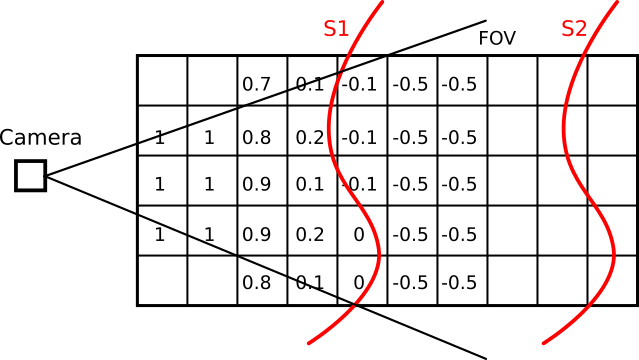
\includegraphics[width=0.55\textwidth]{TSDF}
	\caption[t]{Graphical representation of a voxel grid. Each Grid has a Truncated Signed Distance Function value corresponding to the distance to the nearest surface. In order to avoid interfering with other surfaces, the value assignment to voxels that are far away are taped off after a few voxels}
	\label{fig:TSDF}
\end{wrapfigure}

This method of characterizing reconstruction is very useful for a number of reasons. One can think that given a point cloud, using triangulation (such as Delaunay Triangulation), surfaces would be generated. The problem with simple triangulation methods is that they do not account for noise when collecting range data, and they are harder to incrementally fuse different sets of data. By using weights on each voxel, it was shown in \cite{TSDF} that many scans can be integrated by simply summing the values of the voxels weighted by their respective weight according to a specified weighting function. This makes it easier to integrate different scans and different types of data (for example, Point Clouds and RGBD data), as well as uncertainty based on the defined weight functions of each sensor. Other methods used when adopting this scheme include the concept of the Truncated Signed Distance Function (TSDF \cite{TSDF}), in which the weighting are tapered off behind the surfaces to avoid interference with other surfaces (see Figure \ref{fig:TSDF}).

There are mainly three classes of reconstruction systems that can be seen:
	
\begin{itemize}
\item Active vs Passive Sensors: when using an active sensor (such as Kinect to get RGB-D images), the depth estimates are accurate enough so that a simple fusion using weights is enough to get a good reconstruction (example system KinectFusion \cite{kinectfusion}); when using a passive sensor (such as in DTAM \cite{DTAM}), the depth estimates are usually less accurate and thus there is a need to use a regularizer
\item Object-Centric vs Mobile-Robot-Centric Fusion: when in an object-centric situations, it can be assumed that the voxel block and the voxel grid will be seen all of the time by the sensors (such as in KinectFusion \cite{kinectfusion}). Also, the object is seen in loops multiple times, thus allowing for fine detailed reconstructions; this is not true for a mobile-robot-centric situation, where the robot navigates through the scene instead of around it, and new voxel blocks have to be dynamically allocated depending on the robot's trajectory (such as in Kintinuous \cite{kintinuous}, even though it still uses fixed voxel blocks). It is also unlikely that the same scene is going to be seen multiple times in a range of different angles.
\item Large vs Small Scale: memory allocation plays a huge part when large scale models are used, and that comes at a cost of usually higher voxel sizes, whereas in small scale very small voxel sizes and details can be preserved. Systems that took memory in consideration is the Hashing Voxel Grid (HVG) \cite{HVG}
\end{itemize}
	
Due to the RGB-D sensor becoming widely available as a commodity (as shown in \cite{kinectfusion}), most 3D reconstruction systems have focused on hand-held devices for small scale reconstruction. Since this project relies on LiDAR data, a new system has been chosen.	
	
The system used in this report is BORG-CUBES, which is a reconstruction system that uses sensor-agnostic voxel grids to reconstruct the system. As described in \cite{TannerArXiv2016}, since LiDAR data come at lower frequency than RGB-D data, BORG-CUBES relies on a prior regularizer to improve the quality of the reconstruction. In specific, it uses the Total Variation (TV) regularizer, which penalizes high variations with the assumption that noisy signals have high total variations. It can also integrate stereo visual images, which gives data in higher rates but provide a much lower quality depth map than using LiDAR or RGBD data.	

	\newpage
	\section{System Pipeline} \label{pipeline}

The pipeline for the overall system can be seen below. It consists of 4 modules: (I) First odometry estimates; (II) Laser odometry; (III) Loop closure detection and Graph optimization; (IV) 3D dense volumetric reconstruction.

These 4 modules are broken down in two parts: the first part is concerned about solving the SLAM problem, which outputs a reliable trajectory and map. The second part is concerned with inputting that to a 3D reconstruction system to build the environment volumetrically. Figure \ref{fig:SystemPipelineFigure1} shows the overall system.

\begin{figure}[h]
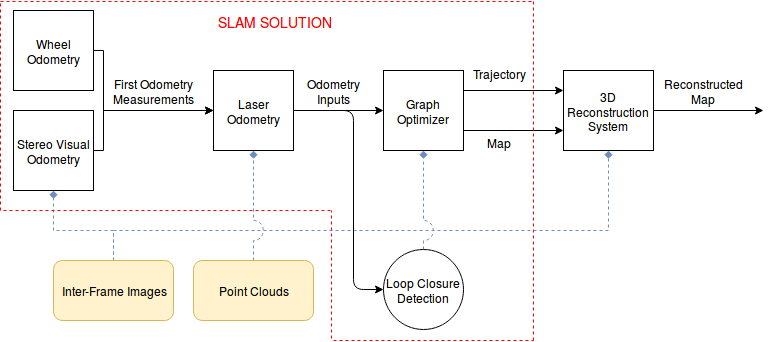
\includegraphics[width=\linewidth]{SystemPipeline}
\caption{Diagram of the overall system pipeline. The beige boxes represent data collected from a sensor, the white boxes represent data being processed and the output being input to the next box. The rounded box is a module built for data association.}
\label{fig:SystemPipelineFigure1}
\end{figure}
	
This pipeline is flexible enough so that many algorithms could be used for each of the modules described above. After consideration about the application of the system - since the goal is to build a mobile robot that reconstructs indoor scenes using LiDAR scans - the algorithms were chosen.
	
For the Visual Odometry, the fovis library \cite{fovis} was use, as it is an open source library that has integration with C++ and works with 3D stereo data, which is used in the MultiSense SL \cite{multisense}, which is the sensor used in one of the tests as described in Section \ref{subs:experiments}.
	
For the Laser Odometry, the algorithm chosen was AICP \cite{7989547}, which works by correcting the odometry measurements by using the ICP algorithm every time a point cloud is available. Since odometry measurements have a significantly higher data rate than the LiDAR sensors used, an algorithm that corrects the poses globally given the laser scans was needed, and the AICP suits this requirement. Further details are going to be explained in Section \ref{subs:LaserOd}.
	
For the graph optimizer, an algorithm that could take into account pose-only SLAM solutions was needed. A full explanation for this is postponed and explained in Section \ref{subs:GraphOpt}. The library used was iSAM \cite{Kaess08tro}, which is an open source library with support to C++, which can solve the problem of pose-only SLAM.
	
Since the system is going to be used only indoors and many loop closures are expected in a relatively short amount of time, a simple loop closure was implemented from scratch, that takes into account heuristics such as Euclidean Distance. The details of this choice is further explained in Section \ref{subs:LoopCl}.
	
The 3D Reconstruction system needs to be able to reconstruct large-scale scenarios. It would be ideal as well to integrate different types of data, since the sensors used in the project allow for stereo and LiDAR data to be available. The framework used then was the BOR\textsuperscript{2}G-CUBES \cite{TannerFSR2015}\cite{TannerArXiv2016}, which is sensor agnostic and implements a regularization term based on Total Variation algorithms to account for non-smooth surfaces. The details of this implementation is shown in Section \ref{sec:Borg}.
		
	\newpage
	\section{SLAM Solution}

As already introduced in Section \ref{pipeline}, the SLAM solution has 4 independent building blocks. This offers sufficient flexibility to test the effect that each part has on the outcome of the map. This section will discuss in more depth how the solution works with all the building blocks working together. 
	 
	\subsection{First Odometry Measurements}

The first odometry measurements offer a relatively inaccurate estimation of the pose of the robot at a certain time. That is because they use methods that are less accurate when compared to laser scans, like stereo vision and wheel odometry (as demonstrated in \cite{achtelik2009stereo} for example in the context of Micro Aerial Vehicles). The purpose of these first estimates is to give an input pose to the Laser Odometry algorithm to perform a better estimate of the trajectory. As shown in Equation \ref{eq:ICPObjective}, the ICP algorithm requires the initial pose of the reference frame of the two point clouds, denoted $X$ and $P$ in Section \ref{subs:ICP}.

Depending on how accurate those poses are, the ICP algorithm can find a global minimum (or get close to it) and offer a fine-tuned estimate of the trajectory. It is important then to get the first odometry measurements as accurate as possible, so that the Laser Odometry can always find a global minimum and make the trajectory optimum.
	
During the project, two methods to get the first odometry measurements were used. When collecting data with the mobile robot Husky \cite{Husky}, the wheel odometry provided by the system served as a good first estimate of its position. When getting the data with the MultiSense SL \cite{multisense}, Stereo Visual Odometry from MultiSense's stereo camera was performed to get the first odometry estimations.
	
	\subsubsection*{Stereo Visual Odometry}

The Stereo Visual Odometry used is based on the system described at \cite{VisualOdometry} and implemented with the fovis library \cite{fovis}. Figure \ref{fig:VisualOdometry1} shows one frame of the result of the visual odometry system when applied to the dataset collected for this project. The inputs came from the stereo camera in the MultiSense SL, collected at 30Hz in a relatively well illuminated indoors scenario.
	
There are a couple of important details that have to be taken into account when implementing the Stereo Visual Odometry. First, an important parameter when using Visual Odometry is the capture time. Since the system has to identify features (corners for example) very efficiently, considerably dark or light streams of images might make this job difficult.  
	
Secondly, the VO usually drifts especially on the pitch and roll directions (as described in \cite{usenko2016direct}. Since the trajectories for this project were mainly across one floor, with flat terrain and mainly two dimensional, the z displacement and the pitch and roll variations were set to zero. The result is a much more accurate 3D map than the one that would be obtained if the 6DOF were being estimated.
	
It is very common to use a combination of Visual and Inertial sensing to get a more accurate estimation of pose. The purpose of using both is that they offer complementary characteristics, mainly with the Inertial system correcting the Euler Angles of the visual estimation. Many examples of such systems can be observed, such as in \cite{usenko2016direct}.
	
\begin{SCfigure}[][ht!]
\begin{minipage}{0.65\textwidth}
\centering
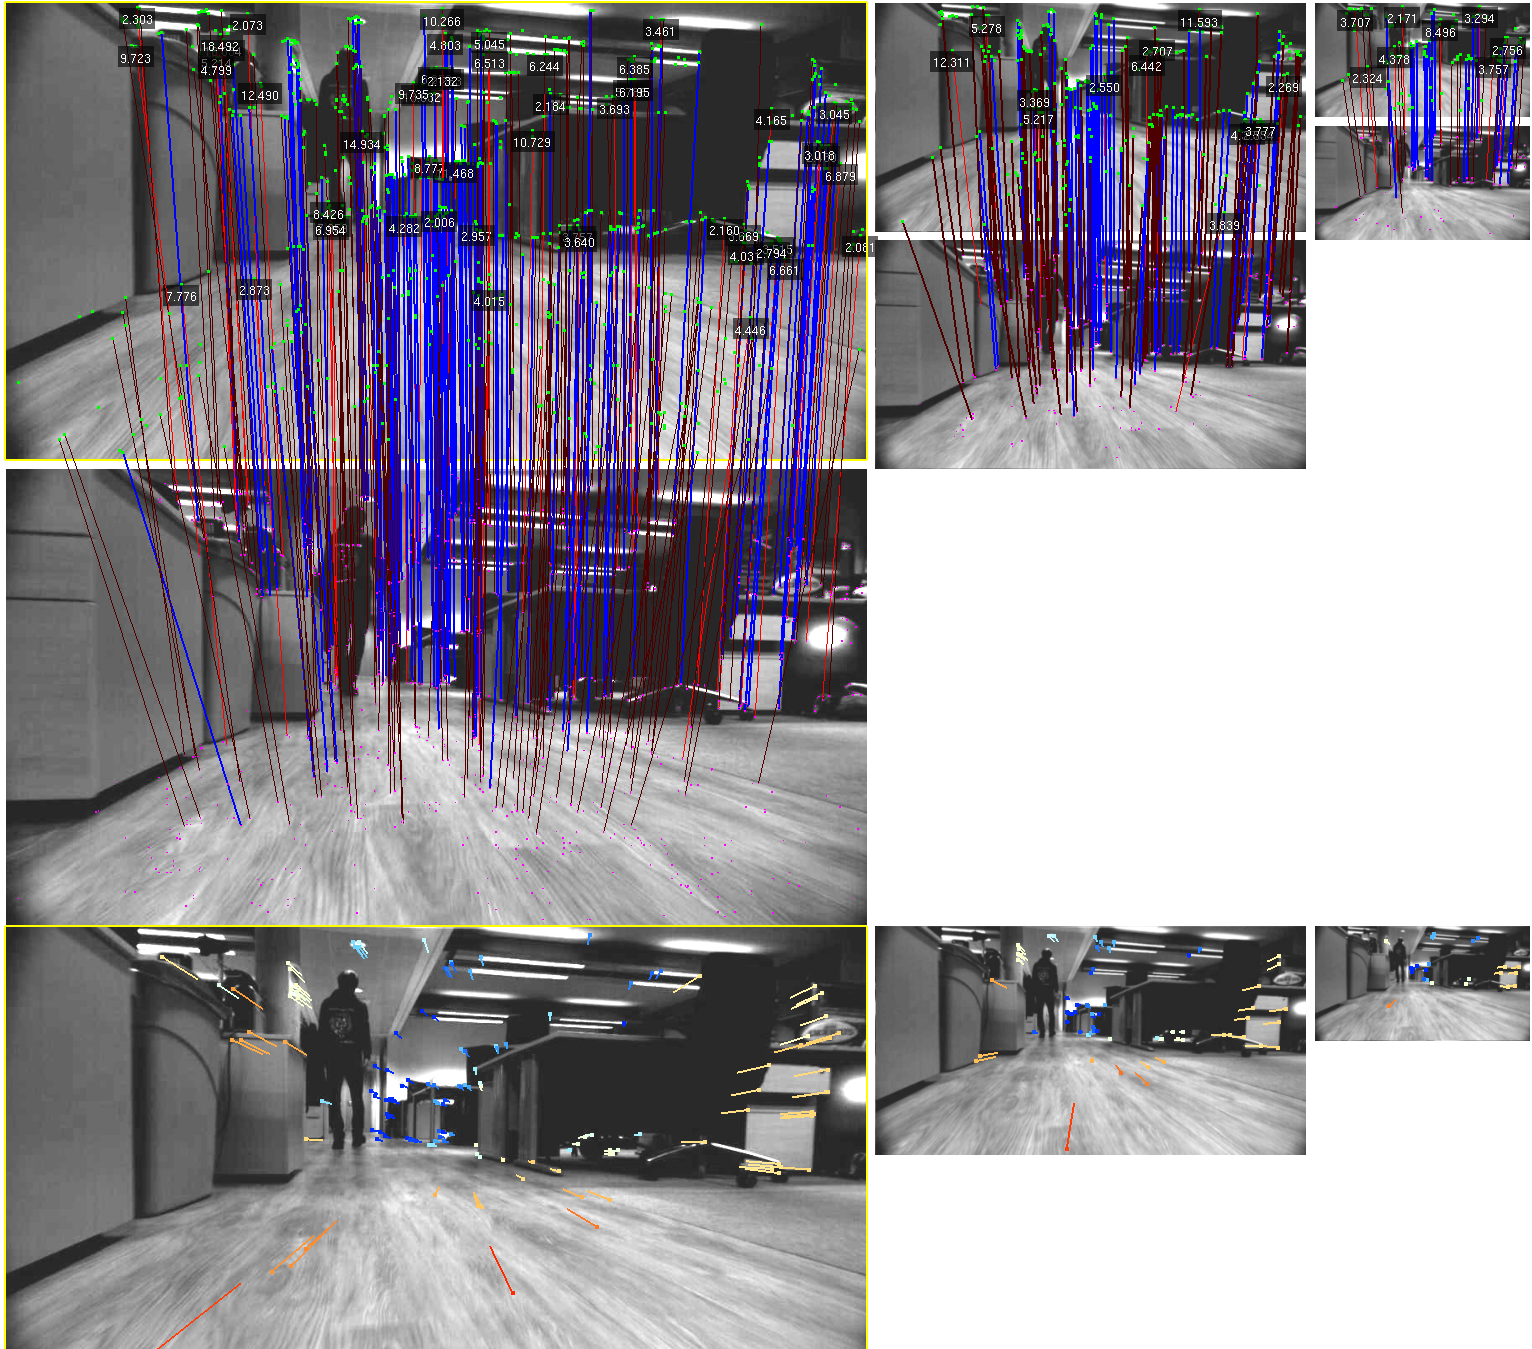
\includegraphics[width=\textwidth]{VisualOdometry1}
\end{minipage} \hfill
\begin{minipage}{0.35\textwidth}
\centering
\caption[t]{Result of fovis library to the data collected at the Information Engineering Building at University of Oxford. The first row of images show a Gaussian Pyramid to extract point features. The Key Frame is shown in the second row where features extracted are matched back to the first row images. Red lines indicate outliers and blue lines indicate inliers (bad and good correspondence respectively). The last row shows the result of the rotation matrix in the pictures. The scale of the movement is indicated as a colour scale from blue to red.}
\label{fig:VisualOdometry1}	
\end{minipage}				
\end{SCfigure}
		
An Inertial Measurement Unit (IMU) was not available at the time of the experiments taken for this project, so such a combination could not be implemented. However, restricting the estimations to two dimensions led to similar results. Further advancements in the project would include having an IMU to make the estimation free in the 6DOF instead of restricting it to 3DOF.
	
	\subsubsection*{Wheel Odometry}

Husky's platform includes a wheel encoder and an IMU, which together implement an EKF estimation of the robot's pose. Since this also just uses proprioceptive sensors, this method makes the robot drift with time. Overall, this method yields similar results to the Stereo Visual Odometry.

An interesting possibility that was not adopted in this project is to integrate both methods to try to get a more precise estimation of the pose. Since the platforms used in this project had a LiDAR sensor available, this was used instead in order to get more accurate estimation results.

	\subsection{Laser Odometry}
	\label{subs:LaserOd}
\textbf{ADD HERE THE MAP WITHOUT ANYTHING APART FORM WHEEL ODOMETRY}
Given the first odometry measurements, it is clear that the resulting map does not look right. In order to improve the estimate of the trajectory, the next step is to use laser based localization using the Point Clouds from the trajectories.
	
Since it uses an exteroceptive sensor, it is expected that laser based localisation achieves significantly less drift than using a proprioceptive sensor (like wheel odometry). However, since ICP algorithms are prone to failure depending on how inaccurate the first pose estimations are, there is a need to incorporate a robust method of incorporating laser based-localization.
	
For this reason, this project used the system described at \cite{AICPAlign} for laser odometry. This algorithm works in two phases: first it selects a point cloud to be the reference of registration. Second, it calculates the prediction of failure of subsequent point clouds to register with the reference. If the prediction states that there is no failure, then the point cloud is registered to the reference, and it iterates to the next point cloud. If the prediction states that there is a risk of failure, then the point cloud becomes the new reference of registration, and subsequent point clouds are registered to this new reference frame.
	
The risk of failure is calculated using two parameters: the alignability and the overlap. First the overlap is calculated using the volumetric overlap of the range and occupancy grid from the first odometry measurements. After that, the alignability is calculated, which is a measure of how ``constrained" in three dimensions the two point clouds are. This is to avoid the problem of registering two point clouds taken in a long corridor for example, where there will be many local minima since the path would be unconstrained in one dimension. From those two parameters, a model is learnt using Support Vector Classifier (SVC), and the Risk Prediction is drawn from that model. More details can be checked at \cite{AICPAlign}.
	
Notice that the algorithm makes the short term drift significantly smaller. The main source of drift in this case is when it predicts high risk failure and have to change the reference of registration. This leaves a small amount of drift at every changing of reference, which accumulates in the long run and yields a noticeable final drift.
	
The results for each of the paths are shown below for comparison. Figure \ref{fig:LaserOdometry1} shows the results for the data collected with Husky using Wheel Odometry. It is noticeable the difference between the accuracy of the First Odometry Measurements to the Laser Odometry. However, it can be seen that there is drift due to how the AICP algorithm works.

\begin{SCfigure}[][ht!]
\begin{minipage}{0.65\textwidth}
\centering
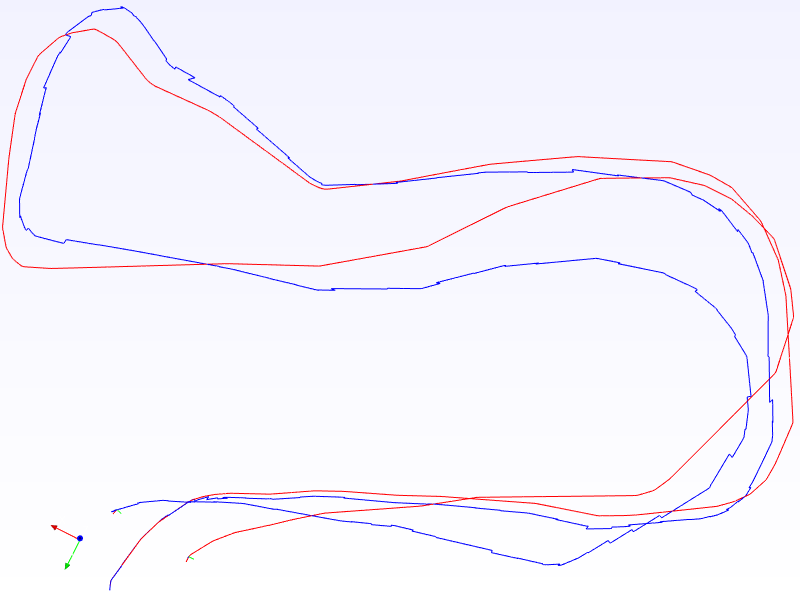
\includegraphics[width=\textwidth]{LaserOdometry1}
\end{minipage} \hfill
\begin{minipage}{0.35\textwidth}
\centering
\caption[t]{Result of the Wheel Odometry feeding the laser odometry system. The red path shows the Wheel Odometry and the blue path shows the corrected poses after being computed by the AICP algorithm. Notice that the corrections are more obvious during the turns, when the wheel odometry is particularly inaccurate.}
\label{fig:LaserOdometry1}	
\end{minipage}				
\end{SCfigure}

This accumulated drift is unnoticeable from frame to frame. However, over a long enough distance, the accumulated drift becomes significant. A way of correcting this long term distance is by using the idea of loop closures.
	
	\subsection{Loop Closure Detection}
	\label{subs:LoopCl}

In order to adjust for the accumulated drift of the path estimate, a loop closure detection algorithm was implemented. Since it was assumed that the robot's drift would not be significantly large (it would not overdrift), three simple heuristics were used to detect loop closure: Time Filter Sampling, Euclidean Distance, and Pose Alignment. 

\begin{itemize}
\item \textbf{Filter Sampling:} In order to avoid the problem of loop closing two state estimates that are in the same room but did not leave the room, a time filter sampling was applied. The idea is to sample every $S$ state estimates, so that the candidate loop closing states would be sparse enough so that the loop just occurs between big time frames, but dense enough to apply euclidean distance.
\item \textbf{Euclidean Distance:} Once the estimates have been  sampled, the euclidean distance between each of them is applied. If the distance between any two states is less than a threshold value $E$, then the two estimates form a candidate pair and they are added in the candidate pair list.
\item \textbf{Pose Alignment:} After the resampling, the candidates pairs are tested for their relative pose. Since the loop closure correction relies on alignment of point clouds using ICP, it is a good strategy to select poses that would maximize the overlap between the point clouds associated with the candidates. In order to do that, another resampling is done based on the overlap between the field of view of the estimates. If the overlap is less than a threshold value $O$, then the candidate pair is dropped out from the list, and the remaining are the loop closures that are considered.
\end{itemize}
	
The parameters $S$, $E$ and $O$ are chosen heuristically depending on what dataset is used in the algorithm. Changing the parameters can affect the outcome of the map significantly, so it is important to spend some time tuning them to the specific requirements of the test.
	
Figure \ref{fig:loopClosureDetection} shows the results of the Loop Closure detection when applied to the Husky dataset. Due to the relatively low velocity of the mobile robot, the parameters were adjusted to match the time that the mobile robot would take to leave a room before coming back to the same room.

\begin{SCfigure}
\begin{minipage}{0.67\textwidth}
\centering
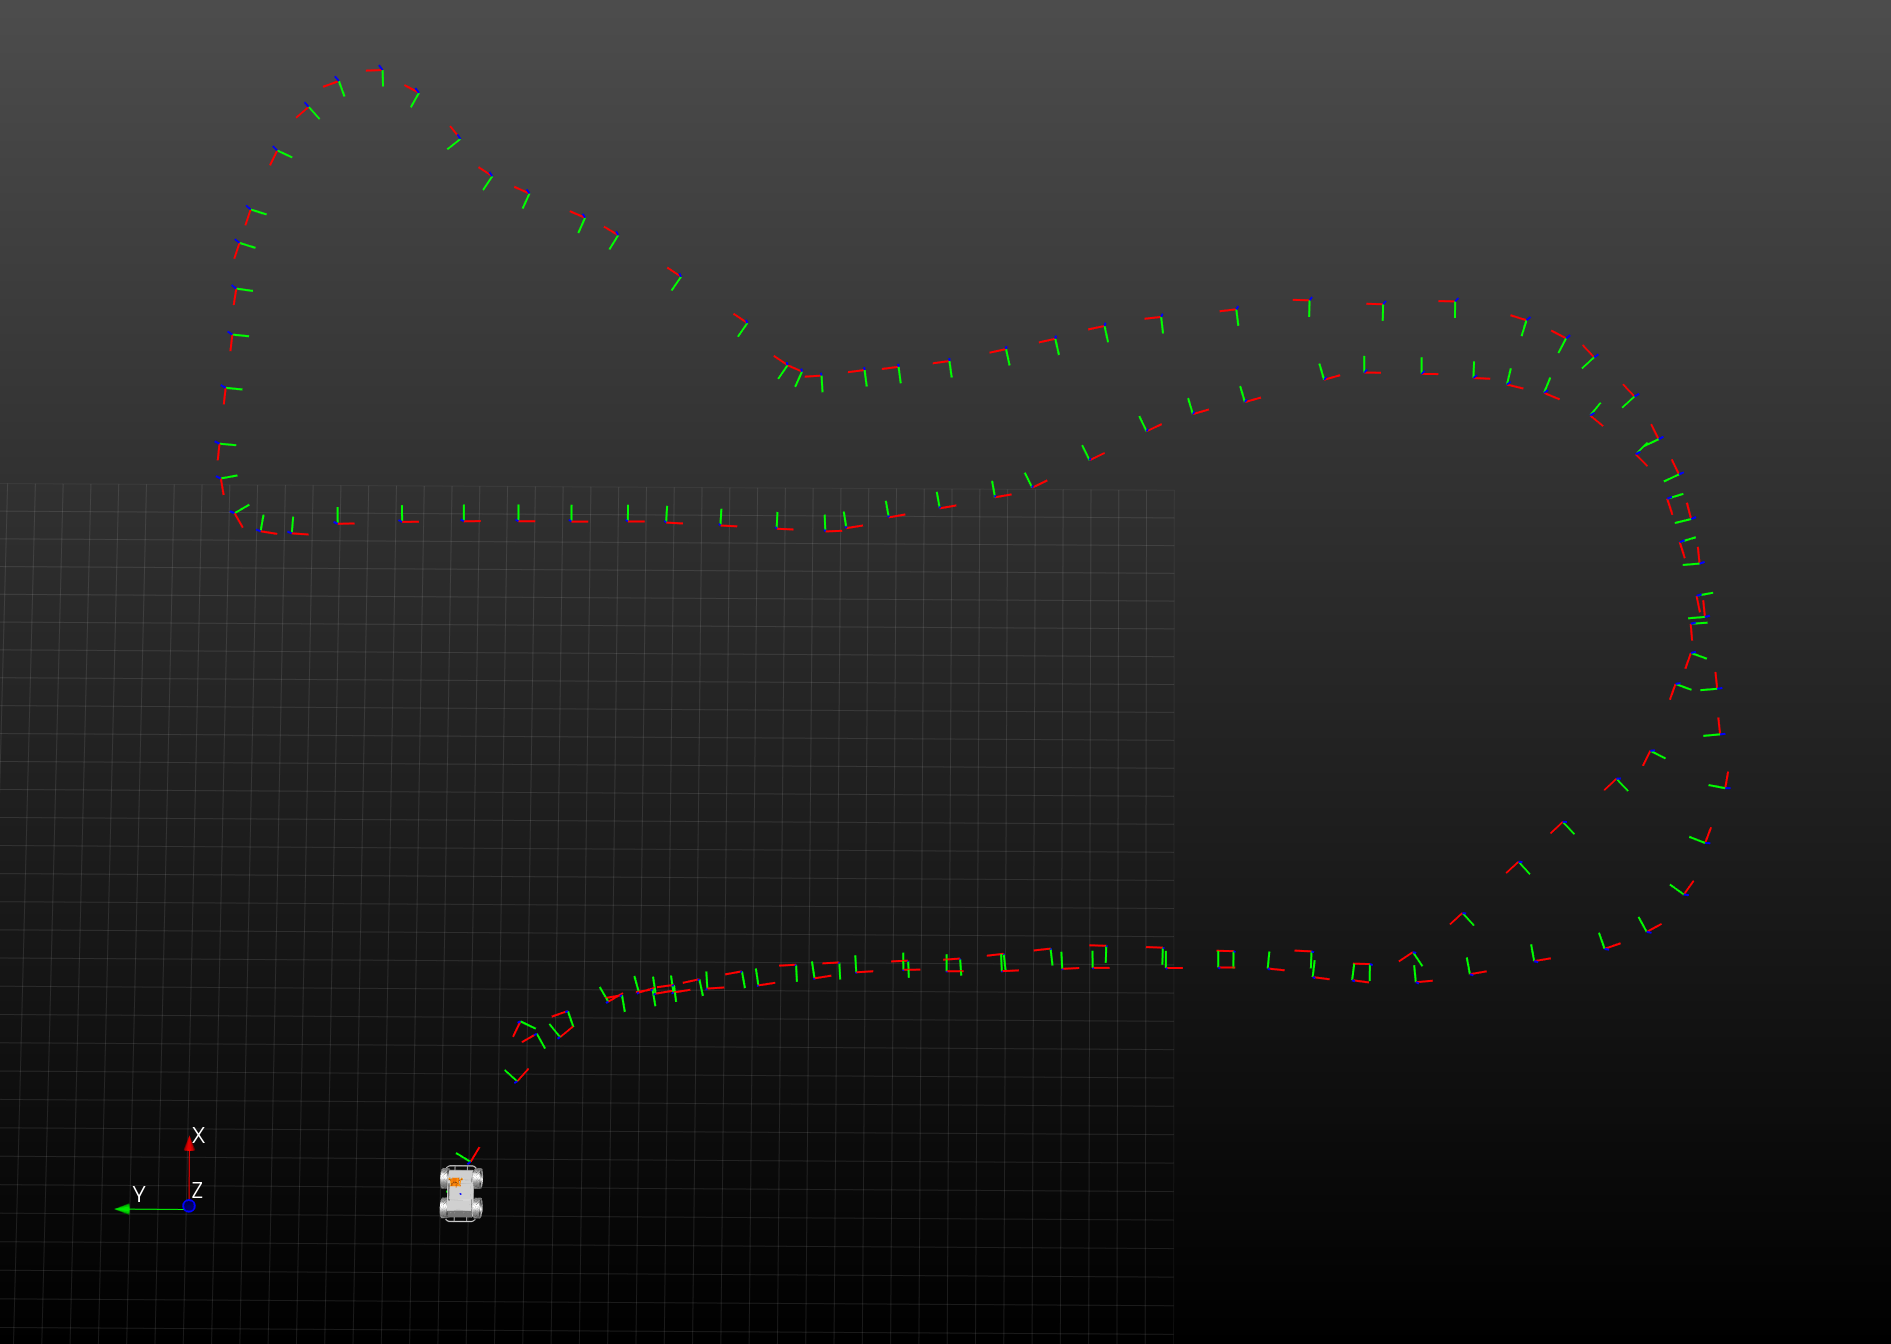
\includegraphics[width=\textwidth]{LoopClosureTimeSampling}
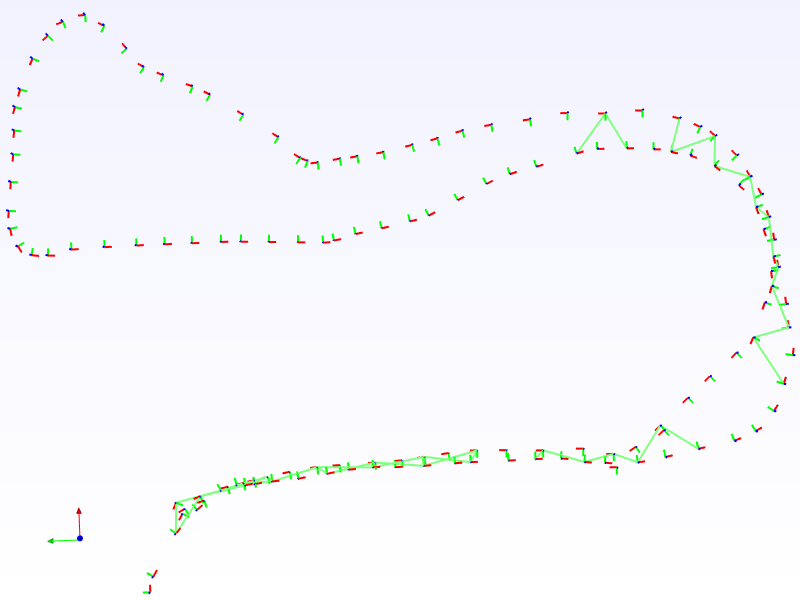
\includegraphics[width=\textwidth]{LoopClosureEuclideanSampling}
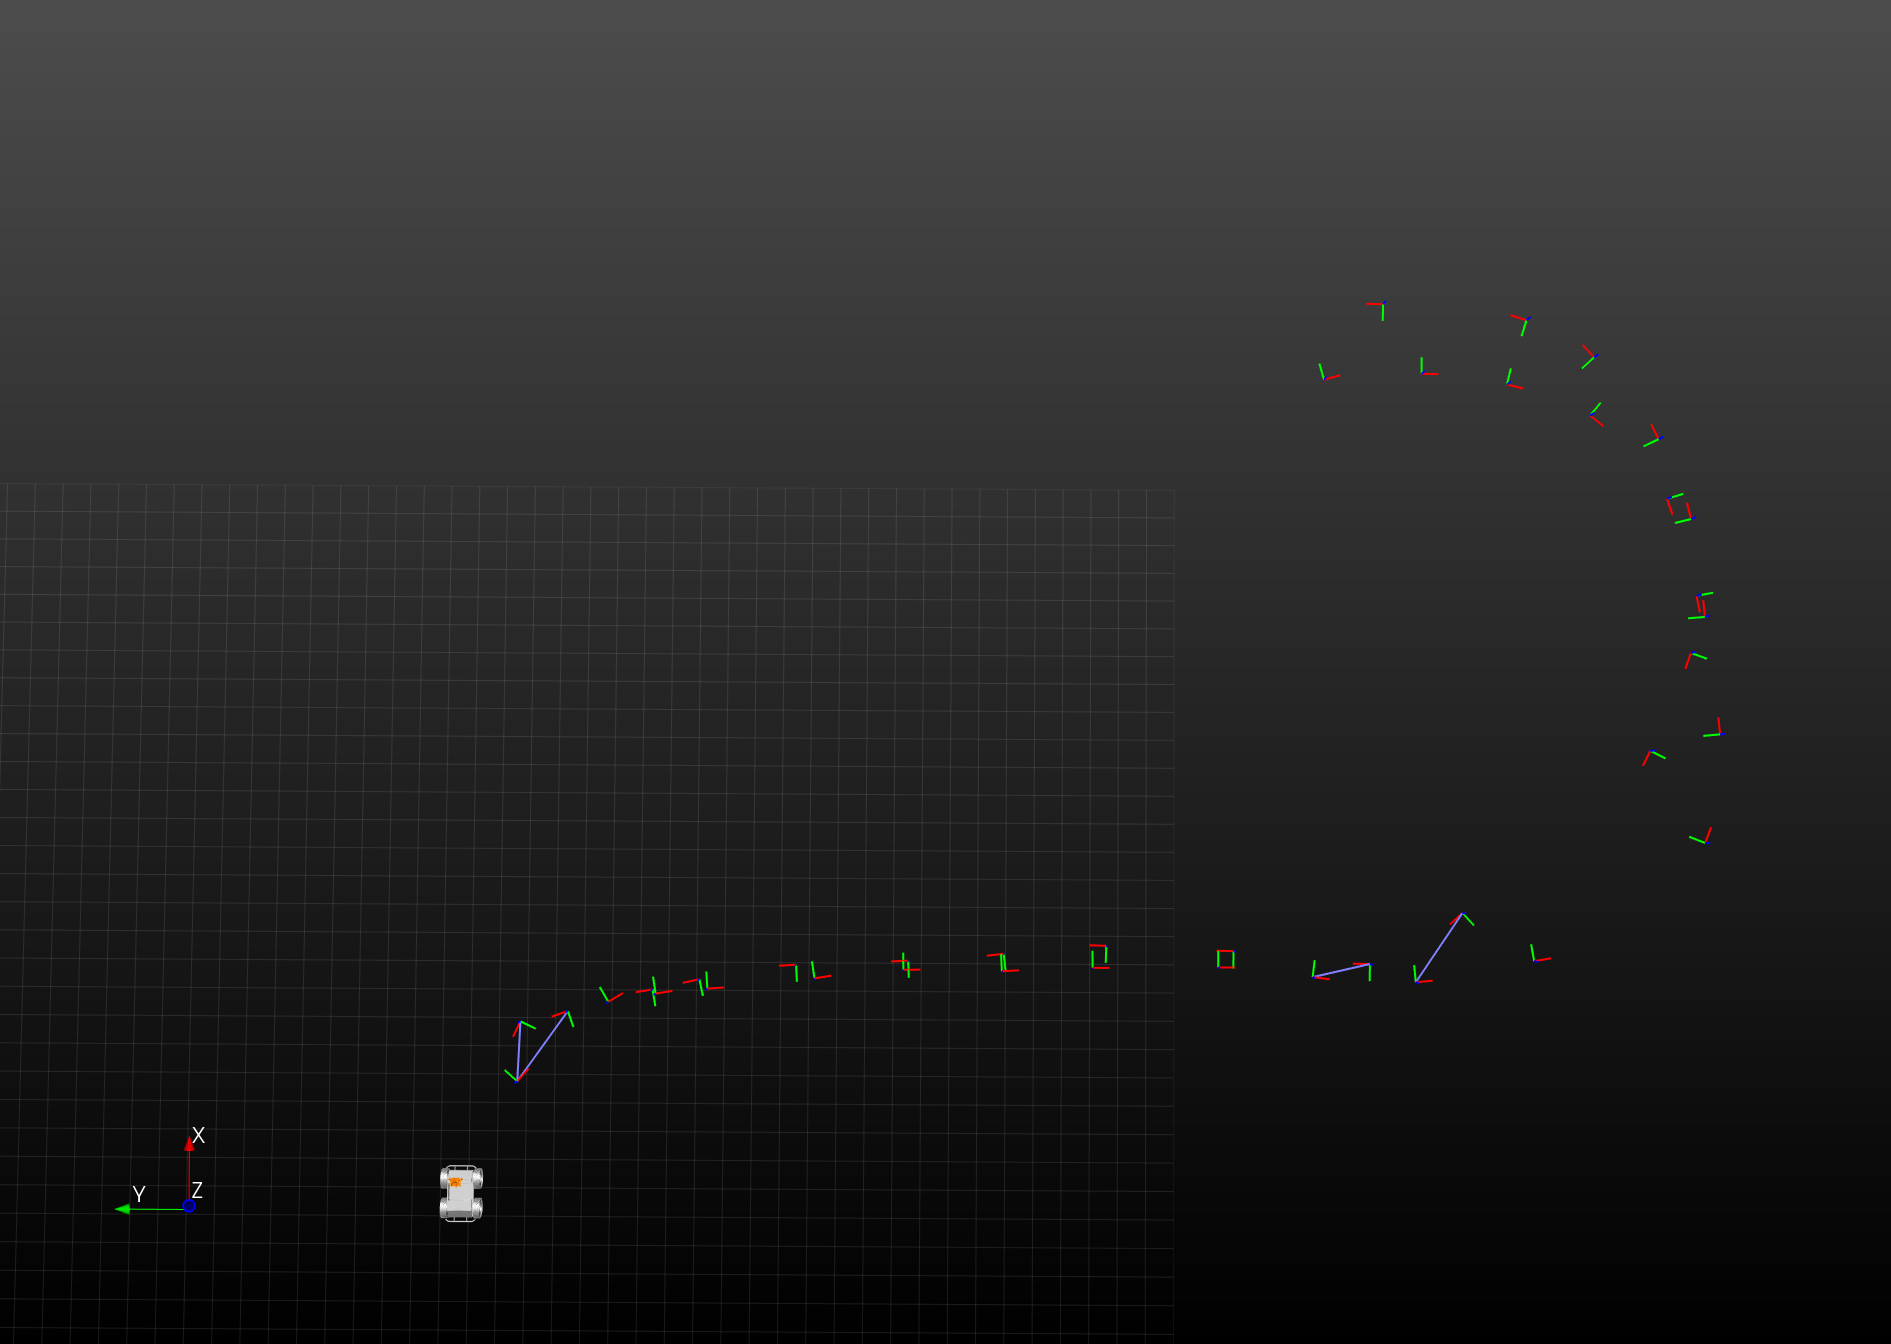
\includegraphics[width=\textwidth]{LoopClosureFinal}
\end{minipage}\hfill
\begin{minipage}{0.33\textwidth}
\centering
\caption[t]{The three heuristics for loop closure detection. Data shown was collected using the Husky Mobile Robot and the Velodyne LiDAR, visualized in bird's-eye view with red and green coordinates representing the path of the robot. The figure on the top shows the result of the time sampling. The plot in the middle shows the Euclidean Distance Pairings. The last figure is the result of the Pose (overlap) filter. In this experiment, $S=2$, $E=2$ and $O=0.5$.}
\label{fig:loopClosureDetection}
\end{minipage}
\end{SCfigure}

It is also important to notice that marginally different parameters have an impact on the number of loop closures and on the outcome of the map. Figure X shows the results of different maps according to different settings of the loop closure parameters.
		
	\paragraph{FIGURE}
	
The assumption that the drift in two loop closures is relatively small is not always valid. For cases when the drift is sufficiently big, other methods for finding loop closures have to be implemented. A popular approach is to find loop closures from images, where each frame is compared given some descriptors and if two scenes look similar enough, they are considered as a loop closure. This is a more sophisticated and accurate system. However, since this project is concerned with indoors mapping, it is assumed that a substantial amount of loop closures will be available in a relatively short time frame. This validates the loop closure system used. Further work in this area would be necessary to make the system more robust to big drifts.	
	
Ideally, the number of loop closures should be neither too big nor too small. Loop closure can be thought of strings ``tightening" the Factor Graph in Figure \ref{fig:slam1} by adding constraints to it. If many loop closures are made, the graph becomes too constraint and new corrections to the map would be insignificant. This can be naively desirable since it means that the certainty of the graph is high, but if one loop closure is a bit off, then the effect cannot be corrected subsequently. In the other hand, if few loop closures are made, then the drift between poses are not corrected substantially and the overall error in the graph is high.
	
Therefore it is crucial to tune the parameters so that meaningful loop closures are selected. 

\paragraph{Front End Loop Closing Problem.} One of the biggest problems with loop closing is that it has a massive effect on the topology of the map. If for some reason either the loop closure is not a good one or if the point cloud registration is inaccurate, the effect on the map is disastrous (just as demonstrated in \cite{latif2013robust}).
	
Unfortunately, ICP algorithms are known for having multiple minima points, which means that not always the registration converges to the global minimum point. Even worse, sometimes the global minimum point might not even be the right registration, maybe due to ambiguities in the map (consider the long-corridor problem and registering a point cloud in the long-corridor).
	
This brought up the problem of multimodaility: because the ICP is not a convex function, there are multiple minima to which the algorithm could converge. In the project, this was demonstrated by slightly perturbing the position of the robot in relation to the previous one. In Figure X below, it can be seen that a small perturbation may make the ICP converge to another minimum point, which means that one of them is wrong. If the wrong registration point is the one detected by the algorithm, then it would introduce an almost irreversible error in the map, and make it more difficult to reconstruct it accurately in the 3D reconstruction system.
	
Many systems and algorithms could be used to avoid this problem, including multihypothesis and a stronger front end selection key. In the project, it was chosen to select the loop closure by hand (i.e. by adjusting the parameters such that appropriate closures are detected) due to the lack of time to implement a multihypothesis system. That is however an area that should be explored in future projects.

	\subsection{Graph Optimization}
	\label{subs:GraphOpt}

As presented in section 2, many graph optimization tools were created. In this project, the Graph Optimization was conducted using the iSAM library. Since the exteroceptive model used was LiDAR data instead of any landmark localizer (like Visual Data or Fiducial Systems for example), a pose-only graph is generated.

A pose constraint-based SLAM follows from the landmark based SLAM. The difference is that instead of using landmarks as a way of localization and mapping, the odometry measurements are used to connect subsequent pose estimates and the loop closures connect two arbitrarily distant poses. This is a common method of SLAM systems when using dense laser range-finder data, such as the LiDAR sensor used in this project. 

Just like with its landmark counterpart, the pose only system can also as easily be modelled using graph models introduced in Section \ref{subs:SLAMRev}. We can model the dependencies of the variables using Bayes Networks as well.
	
\begin{SCfigure}[][ht!]
\begin{minipage}{0.65\textwidth}
\centering
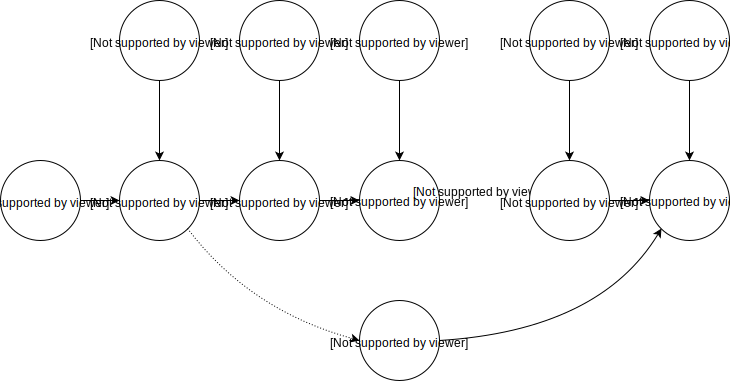
\includegraphics[width=\textwidth]{BayesNetSLAMPoseOnly}
\end{minipage} \hfill
\begin{minipage}{0.35\textwidth}
\centering
\caption{Pose only SLAM as a Bayes Net. The dotted line from $x_1$ to $c$ represents the parameter used for the loop closure. The value $\mathbf{x_0}$ denotes a prior; $\mathbf{x_n}$ denotes the state vector; $\mathbf{u_n}$ denotes odometry measurements; $\mathbf{c}$ denotes close loops.}
\label{fig:slam2}
\end{minipage}				
\end{SCfigure}

Framing the model above mathematically, the total probability is given by:

\begin{equation}
P(X,U,C)\ \propto \ P(x_0)\prod_{j=1}^{M}P(x_j|x_{j-c},c_j)\prod_{i=1}^{M}P(x_i|x_{i-1}, u_i)
\label{eq:probSLAM2}
\end{equation}
	
The loop closures $C_j$ act just like a odometry measurements. They are computed using the ICP algorithm as described in \ref{subs:LoopCl}. They are treated separately in the iSAM algorithm, which includes another constraint to the system. As described in \cite{Kaess08tro}, loop closures add a lot of non-zero entries in the factor matrix when landmarks are used. This results in added complexity and increase of computational burden. However, they are very important for long-term drift free localization and mapping, as discussed in Section \ref{subs:SLAMRev}. It is important to notice that all of the SLAM properties for landmarked based systems also hold for Pose-Only based systems \cite{Kaess08tro}.
	
The results of the Wheel Odometry system when applied the Optimization are shown in the Figure \ref{fig:GraphOptimization1}. Both figures show the  point clouds collected in the experiment, which can be used to understand how well the localization algorithm performs. In the figure on the left, the different colours represent different timestamps in which the point cloud was taken, starting with blue, going to orange, then blue, yellow, and finishing with red.
	
\begin{figure}[ht]
\centering
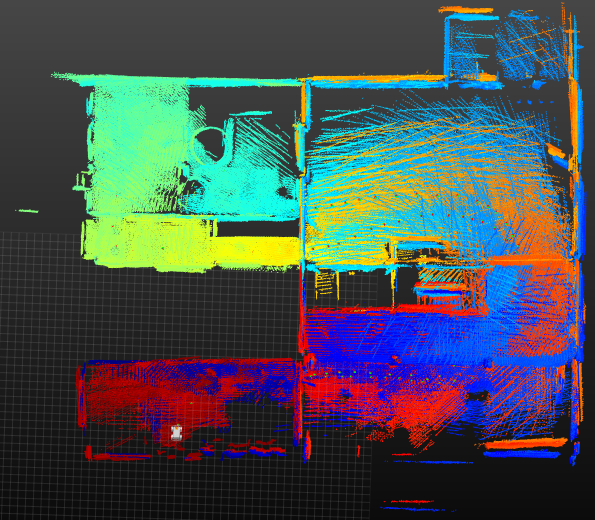
\includegraphics[width=0.48\textwidth]{ResultNoLoopClosure}
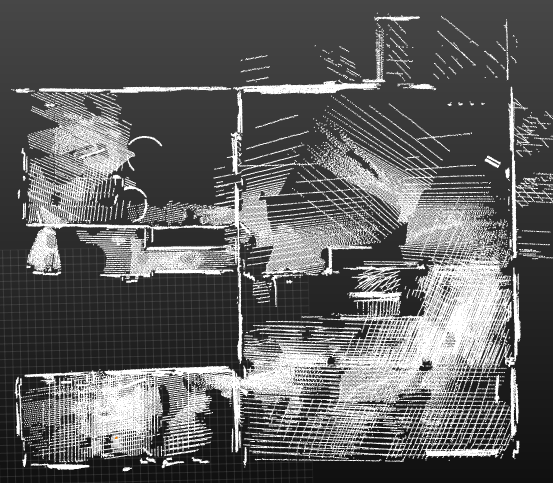
\includegraphics[width=0.48\textwidth]{ResultLoopClosure}
\caption{Result of the Graph Optimization solution. The map in the left shows the Point Clouds collected without Graph Optimization and Loop Closures applied. The map in the right shows the result of the map after the loop closures have been implemented in the iSAM algorithm. Notice the alignment of the wall at the top of both images and at the very bottom to compare the overall drift of both systems. The point clouds in the picture in the left are coloured with timestamps.}
\label{fig:GraphOptimization1}	
\end{figure}
	
It can be clearly seen that the figure on the left does not show any apparent drift in the short term. Each of the individual close point clouds seem to be aligned. This can be noticed by looking at point clouds of the same colour. For example, the point clouds with orange colour seem to be perfectly aligned with each other. This indicates that short term drift is small.
	
However, when comparing point clouds that have different colours (for example, the blue and the red), it is clear that in the long term, the robot has drifted significantly. This long term drift is only apparent when the robot goes back to the same room, which can be detected using the algorithm as described in Section \ref{subs:LoopCl}.
	
The figure on the right shows the map after the point clouds have been aligned. Comparing the bottom right corner of the two figures (the red and blue point clouds) and the top right corner (the cyan and orange point clouds), it can be seen that the figure in the right manages to align the long term drifts satisfactorily.
	
This is an important result, since global alignment of the point clouds is crucial for the 3D reconstruction described in the next section. In this way, we avoid doubled walls and open the opportunity for more flexibility when defining the hyperparameters of the 3D Reconstruction System.
	
	\newpage
	\section{Integration with BOR\textsuperscript{2}G-CUBES}
	\label{sec:Borg}
	
As explained in Section 3, the result of the Graph Optimization is then input to BORG-CUBES. Since this algorithm was built to reconstruct cities with an eye at autonomous driving, it expects a pretty dense representation of the LiDAR point clouds. Unfortunately, this is not the case for mobile robots operating indoors with a single LiDAR sensor.
	
On top of that, BORG CUBES adopts a framework that can regularize the reconstruction based on the Total Variation. Putting it simple, the idea is to optimize a cost function that penalizes high derivatives. It is of the form below:


\begin{equation}
\underset{u}{min} \int_{\Omega } | \nabla u| d \Omega + \frac{\lambda}{2} \int_{\Omega}||u_i - f_i||^2 d \Omega
\label{eq:Regularizer}
\end{equation}

In the equation above, the first term shows the total variation cost. This is the term that emphasizes that the data must be changed to make it smoother. The second term is the data fidelity cost. That term is responsible to make the structure resemble the observations of the data.

The hyperparameter $\lambda$ is set by the user and it dictates how much weight each of the two terms are going to have. Different than a normal regularization framework, this term sets how much fidelity to the data the regularized model is going to have. A high value for $\lambda$ indicates that the model should be closer to the unregularized model even though it might mean being noisy. A low value for $\lambda$ means that the regularized model should be smoother, even though it means being less similar to the data.

Figure \ref{fig:Regularizers} shows some results of changing the lambda parameter for some models. Even though regularizing the map yield a smoother reconstructed surface, it also excludes surfaces that are in general disconnected from other surfaces, as can be seen in the next figures.

\begin{figure}[h]
	
	\begin{tabular}{cccc}
	\subfloat[$\lambda \to \infty$]{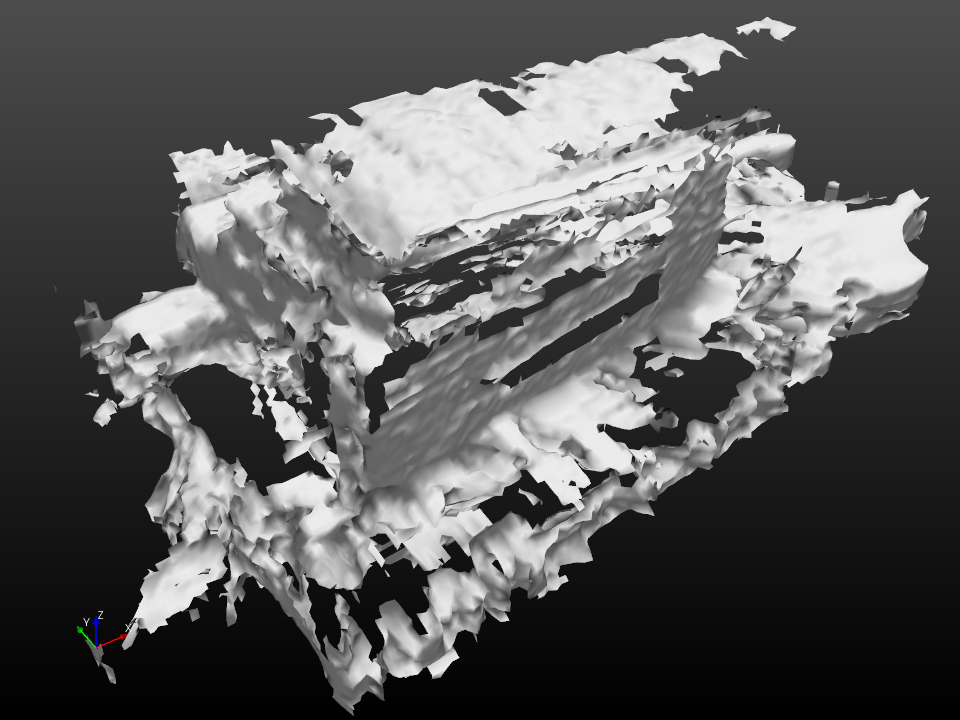
\includegraphics[width = 0.5\linewidth]{Regularizer/Unreg}} &
	\subfloat[$\lambda = 1$]{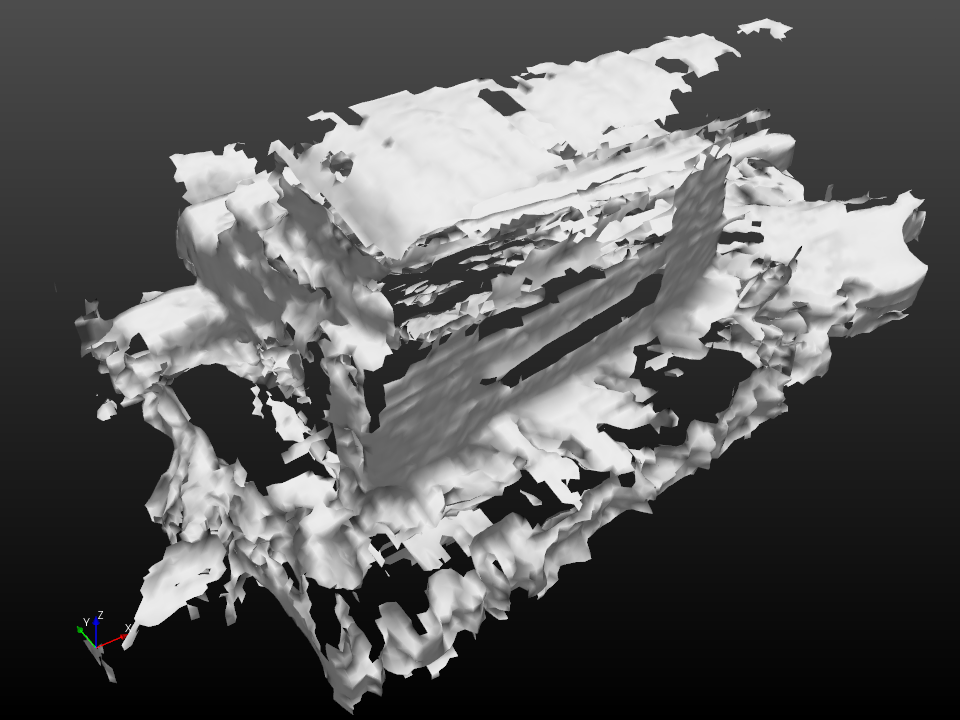
\includegraphics[width = 0.5\linewidth]{Regularizer/1Lambda}}\\
	\subfloat[$\lambda = 0.5$]{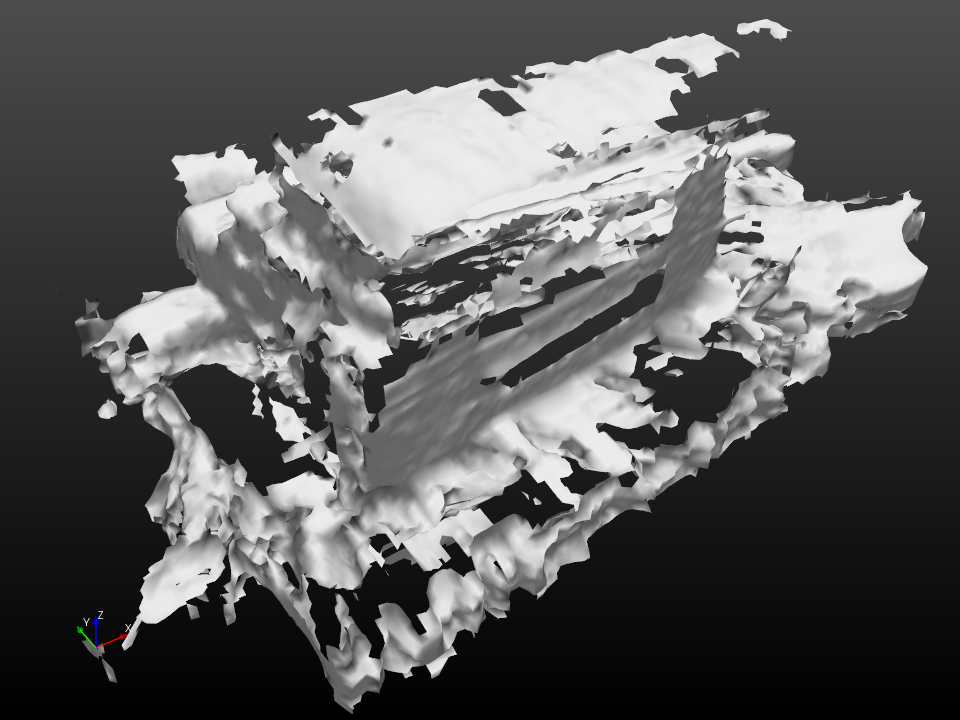
\includegraphics[width = 0.5\linewidth]{Regularizer/05Lambda}} &
	\subfloat[$\lambda = 0.1$]{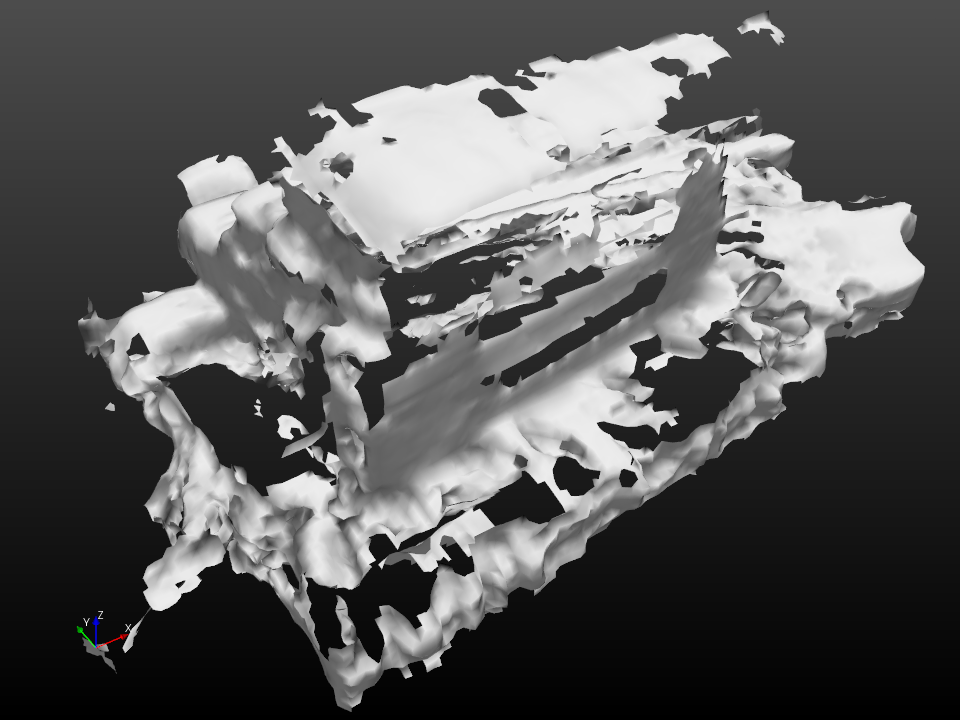
\includegraphics[width = 0.5\linewidth]{Regularizer/01Lambda}}
\end{tabular} 
	\caption{Model with different $\lambda$ values for the regularizer. It can be seen that the surfaces get smoother the smaller the value of $\lambda$ is.}
	\label{fig:Regularizers}
\end{figure}

There are also a couple of hyperparameters that needs to be set when using any 3D reconstruction system. The most important one is the edge length. This sets the size of each voxel in the voxel grid. The bigger this number is, the more "pixelized" the reconstruction is going to be. The smaller this number is, the more detailed it is going to become. There is an important trade-off when setting this number. For object-centered small-sized reconstructions, such as KinectFusion \cite{kinectfusion}, a small side-length of the voxels would mean more fine details of the reconstructed scene. KinectFusion for example sets this value to	 1.95mm, so that a $256^3$ voxel block would mean a $0.5^3 m^3$ volume. For large scales though, that would mean too much memory having to be allocated. BORG Cubes for example sets the size length to 0.2m.
	
Figure \ref{fig:Voxels} shows the result of different edge lengths applied to a model. It can be seen that the lower the value of the voxel edge, the more detailed the model becomes. However, this results in sparser surfaces, since small voxel sizes mean that many of them are empty, which results in unconnected surfaces. A very large voxel size might result in surfaces being blended such that the overall shape of the building is not properly captured.

\begin{figure}[h]
	
	\begin{tabular}{cccc}
		\subfloat[Voxel edge = $10cm$]{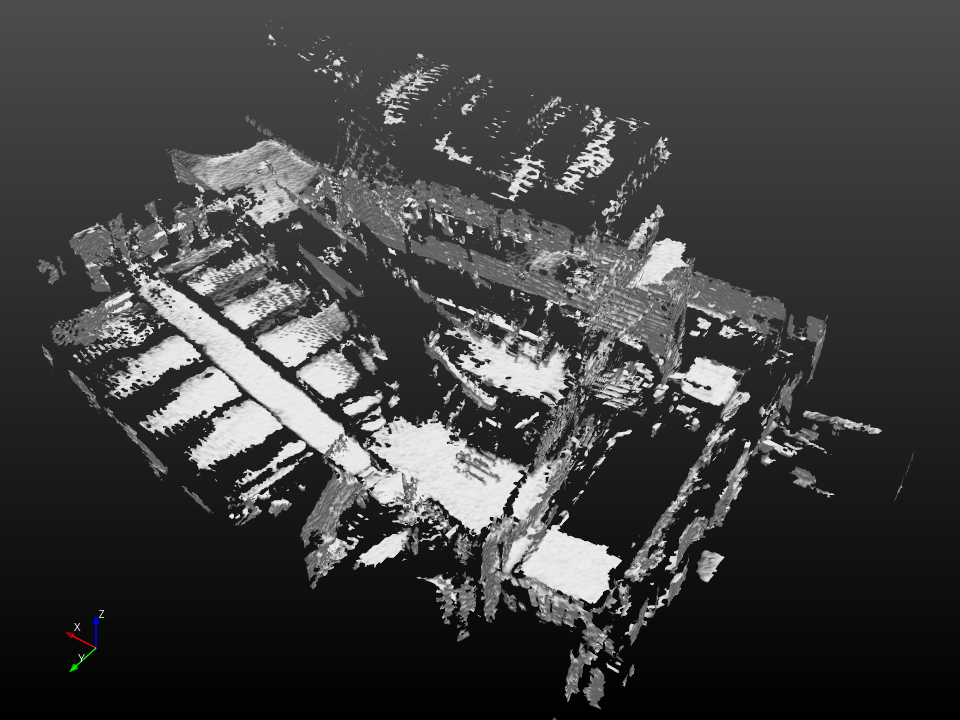
\includegraphics[width = 0.5\linewidth]{VoxelEdge/Voxel01}} &
		\subfloat[Voxel edge = $30cm$]{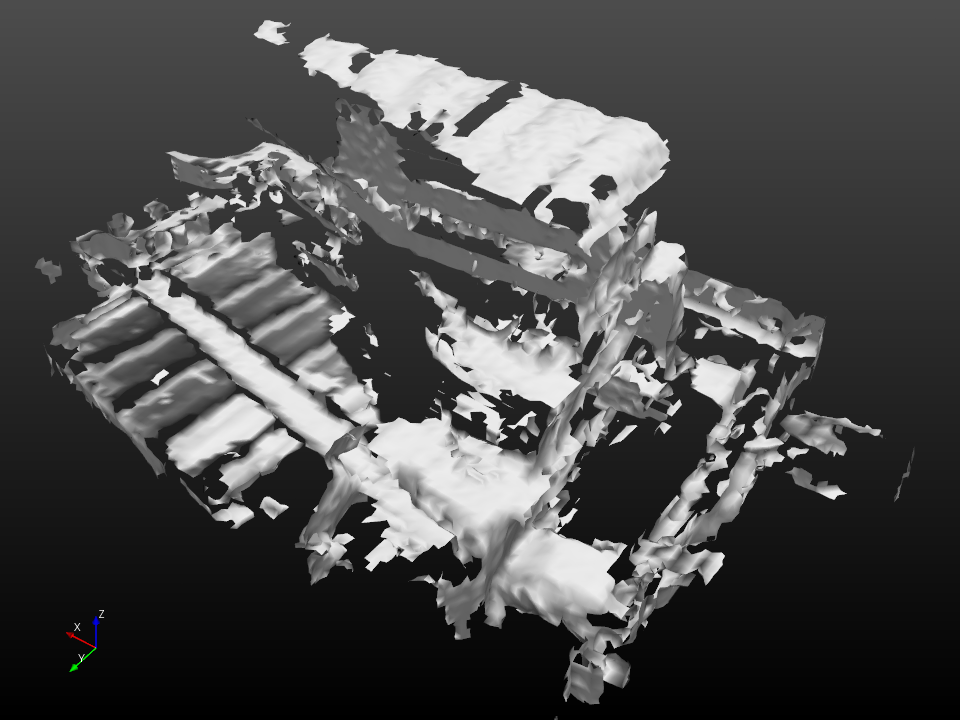
\includegraphics[width = 0.5\linewidth]{VoxelEdge/Voxel03}}\\
		\subfloat[Voxel edge = $50cm$]{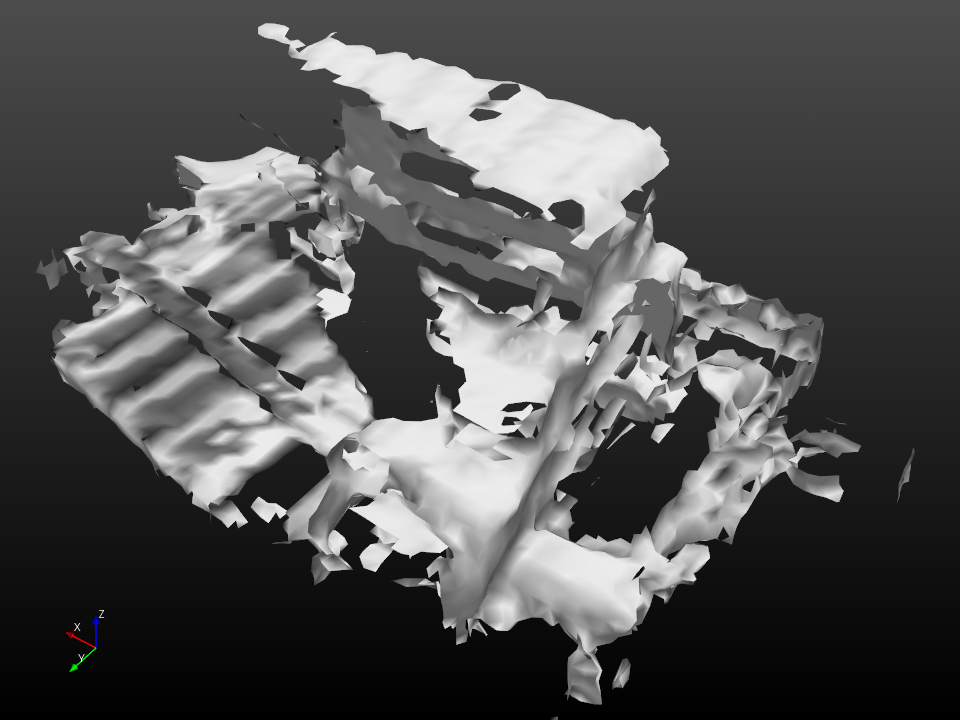
\includegraphics[width = 0.5\linewidth]{VoxelEdge/Voxel05}} &
		\subfloat[Voxel edge = $1m$]{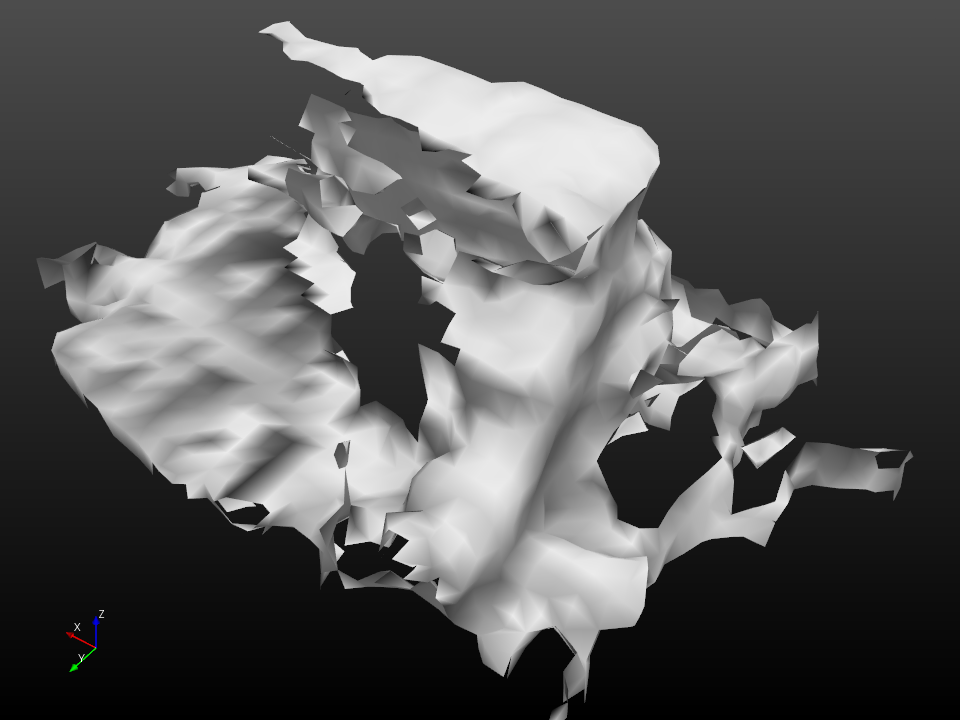
\includegraphics[width = 0.5\linewidth]{VoxelEdge/Voxel1}}
	\end{tabular} 
	\caption{Models with different Voxel Edge Length values for the fusion.}
	\label{fig:Voxels}
\end{figure}

Ideally, we would expect that smaller voxel edges would make the reconstruction look more realistic. Such as demonstrated in KinectFusion \cite{kinectfusion}, very small voxels yield models that closely resemble reality. When reconstructing big environments though, a bigger importance is placed on the overall shape of the building rather on the small details. One could say that for planning in big environments, low frequencies should outweigh high frequencies. 

Also as expected, the determination of all of these aforementioned hyperparameters is more of an art than a science. Different parameters might work better in different environments and applications, using sensors with different accuracies. In general, large-scale reconstructions require larger voxel edge lengths to account for limited memory, and the $\lambda$ regularization term varies between 0.5 to infinity (which is basically no regularization), which can account for limited computation power.
			
	\newpage
	\section{Experimental Results}
	\label{subs:experiments}

This pipeline was tested in two different datasets: the Edinburgh dataset and the Information Engineering Building (IEB) dataset. In both of them, the sensors did not contribute to planning nor control of the robots, but rather they were moved independently for the data collection.
	
The sensor used to collect these datasets was the MultiSense SL \cite{multisense}, which is a tri-modal sensor: it provides laser data, - from a Hokuyo UTM-30LX-EW - 3D stereo data, and RGB video. The laser spin was set to 15RPM for both of the datasets. The aperture time for the stereo camera can be changed, and in both of them it was set so that it would compensate the light condition of the experiments. 
	
	\subsection{Edinburgh Dataset}

This dataset is the same used at \cite{AICPAlign} - called the IF dataset in the paper. This is an approximately 180 meters path. It passes through 5 doorways in 5 different rooms of varying sizes. It collects data in an area of approximately 27m x 32m, with a maximum height of approximately 20 meters, which are achieved in the two big rooms. It contains static objects (such as tables and chairs) and moving people. It is a one big loop path, which is convenient for the loop closure detection.
	
There were 117 scans in total, each having approximately 6000 points. A top view of the map is shown in Figure \ref{fig:TopViewEdinDataset}. The numbers are labelling the different rooms of the environment. In the experiment, the robot travelled from rooms 1 to 5, and returned to 3, then 2 and finally 1. As it was explained in Section \ref{subs:LoopCl}, the parameters to select the loop closures play an important role when compiling the final map. In this case, the parameters were set so that 5 loop closures were identified: one in room 3, two in room 2 and two in room 1. When compared to the map shown at \cite{AICPAlign}, it is clear that there is no accumulated drift due to odometry measurements in room 1. The map created then is accurate enough to be the input to the reconstruction algorithm.
	
\begin{figure}
\centering
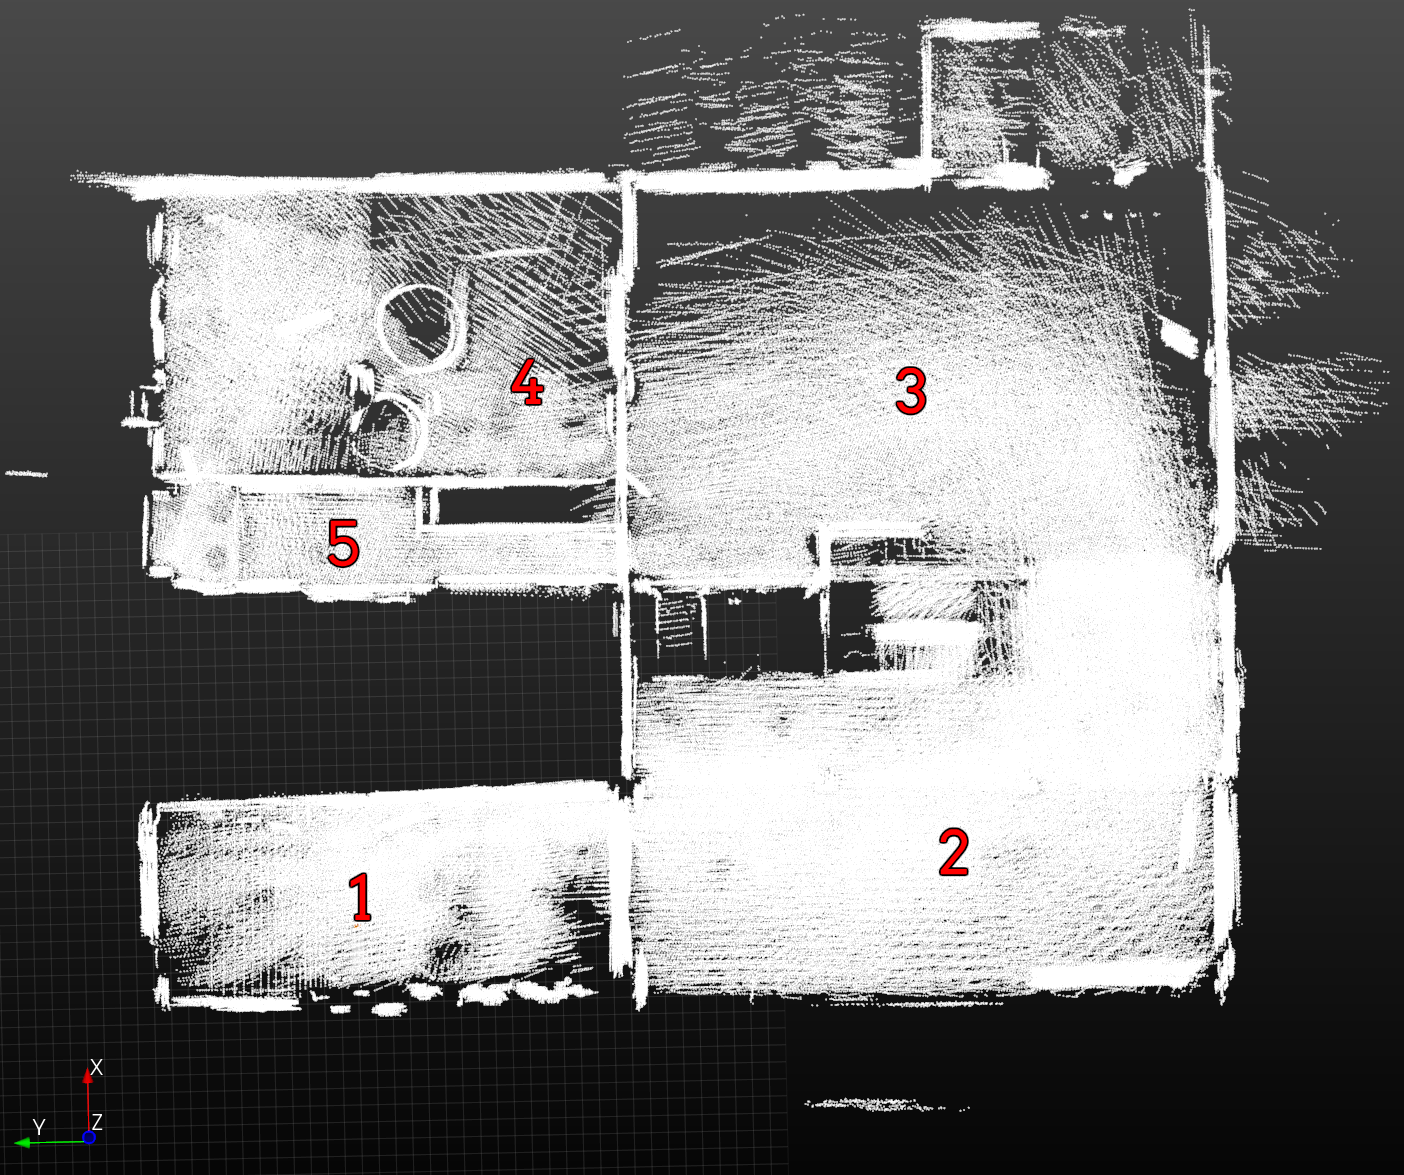
\includegraphics[width=0.8\linewidth]{Maps1/TopViewMarked}
\caption{Bird's Eye view of the map of the Edinburgh Dataset. The path taken was 1, 2, 3, 4, 5, 3, 2, 1. Loop Closures were detected in rooms 3, 2 and 1.}
\label{fig:TopViewEdinDataset}
\end{figure}
	
The results of the final reconstruction of this system is shown in Figure \ref{fig:EdinbDataset}. The first row of the figure contains the raw point clouds collected and arranged after the SLAM algorithm output the trajectory of the robot (with loop closure included). It can be seen that even though the point clouds are dense in the some walls and in some of the roofs, there are some areas of sparseness. In particular, corners, windows and some of the walls do not have or hardly have any points at all. This is expected, since the laser data only collects points if the laser is reflected back to the sensor, which might leave holes depending on the surface that it is trying to reconstruct.
	
\begin{figure}
\centering
\caption*{\textbf{Edinburgh Dataset}}
\begin{tabular}{cccc}
\subfloat{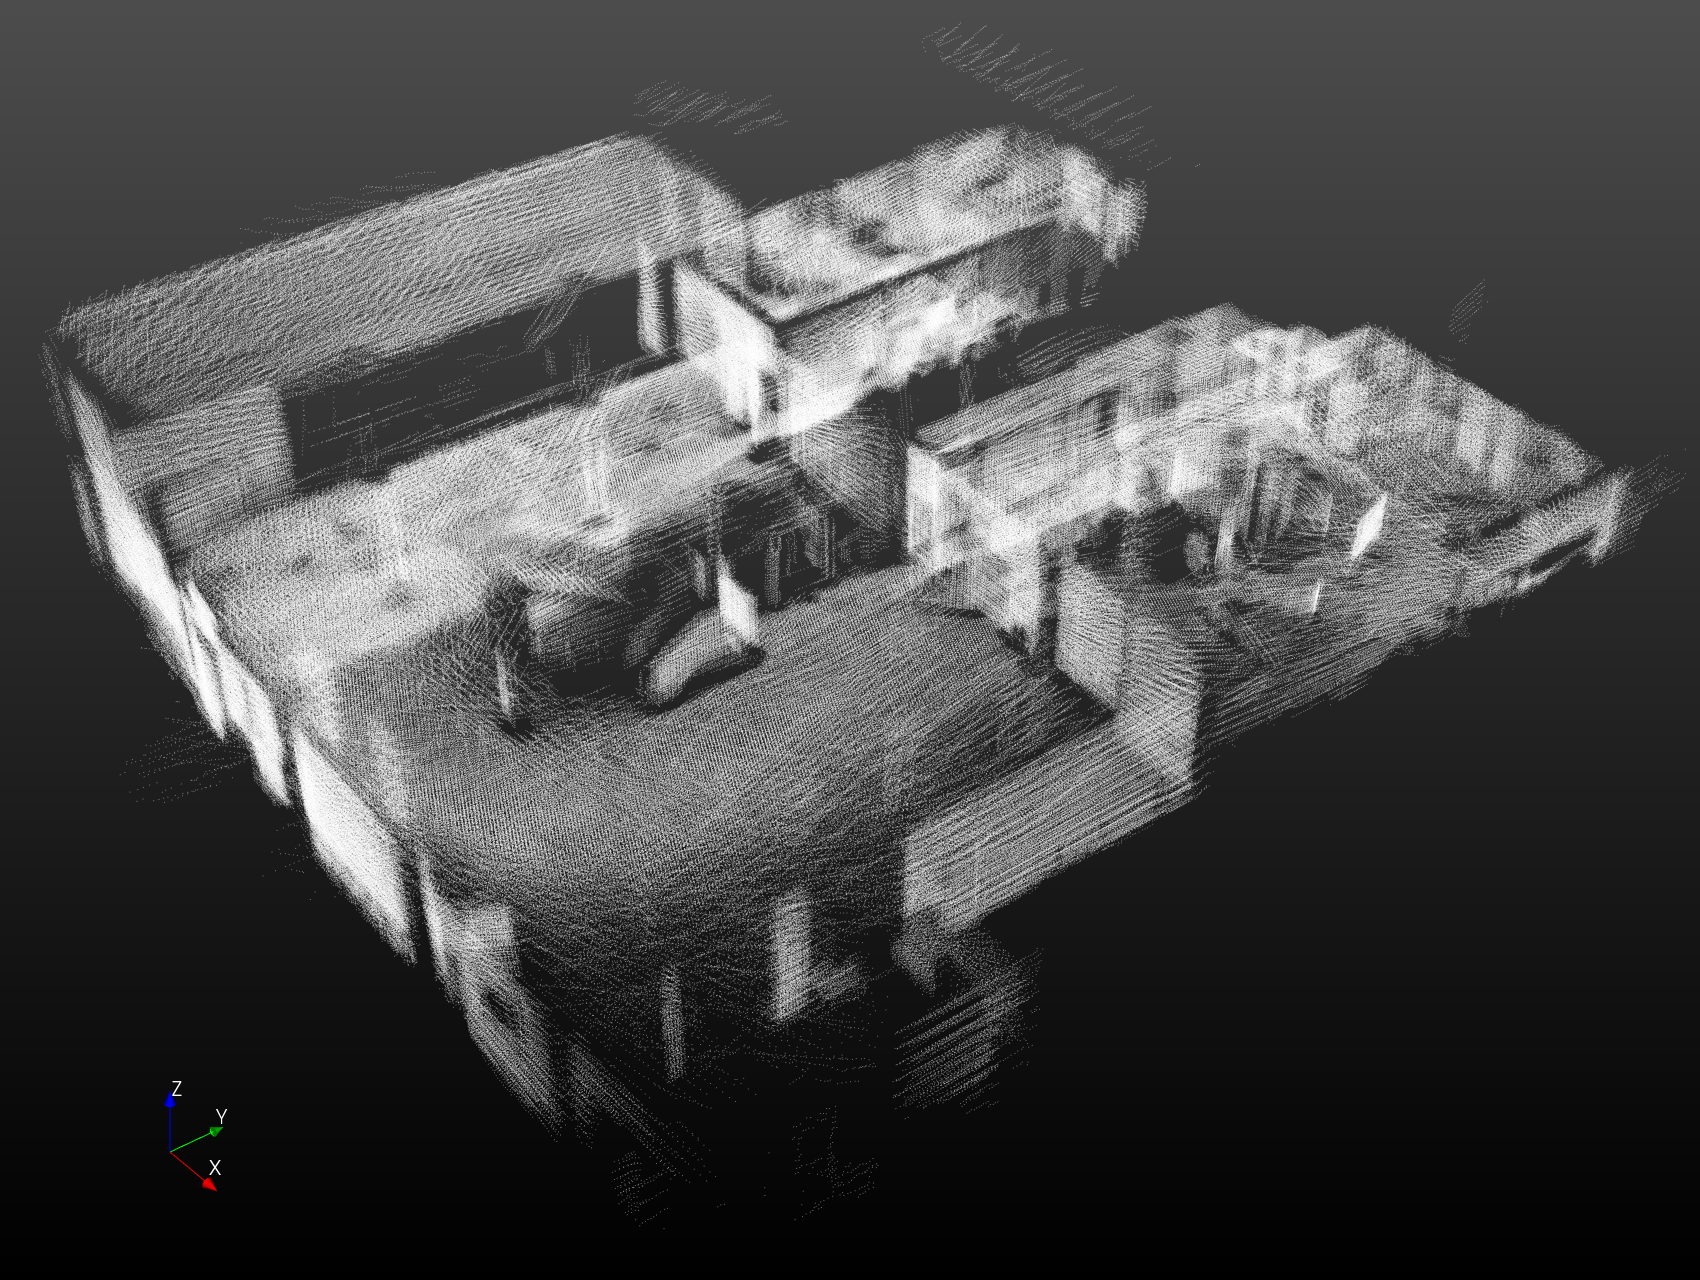
\includegraphics[width = 0.3\linewidth]{Maps1/PTCL1}} &
\subfloat{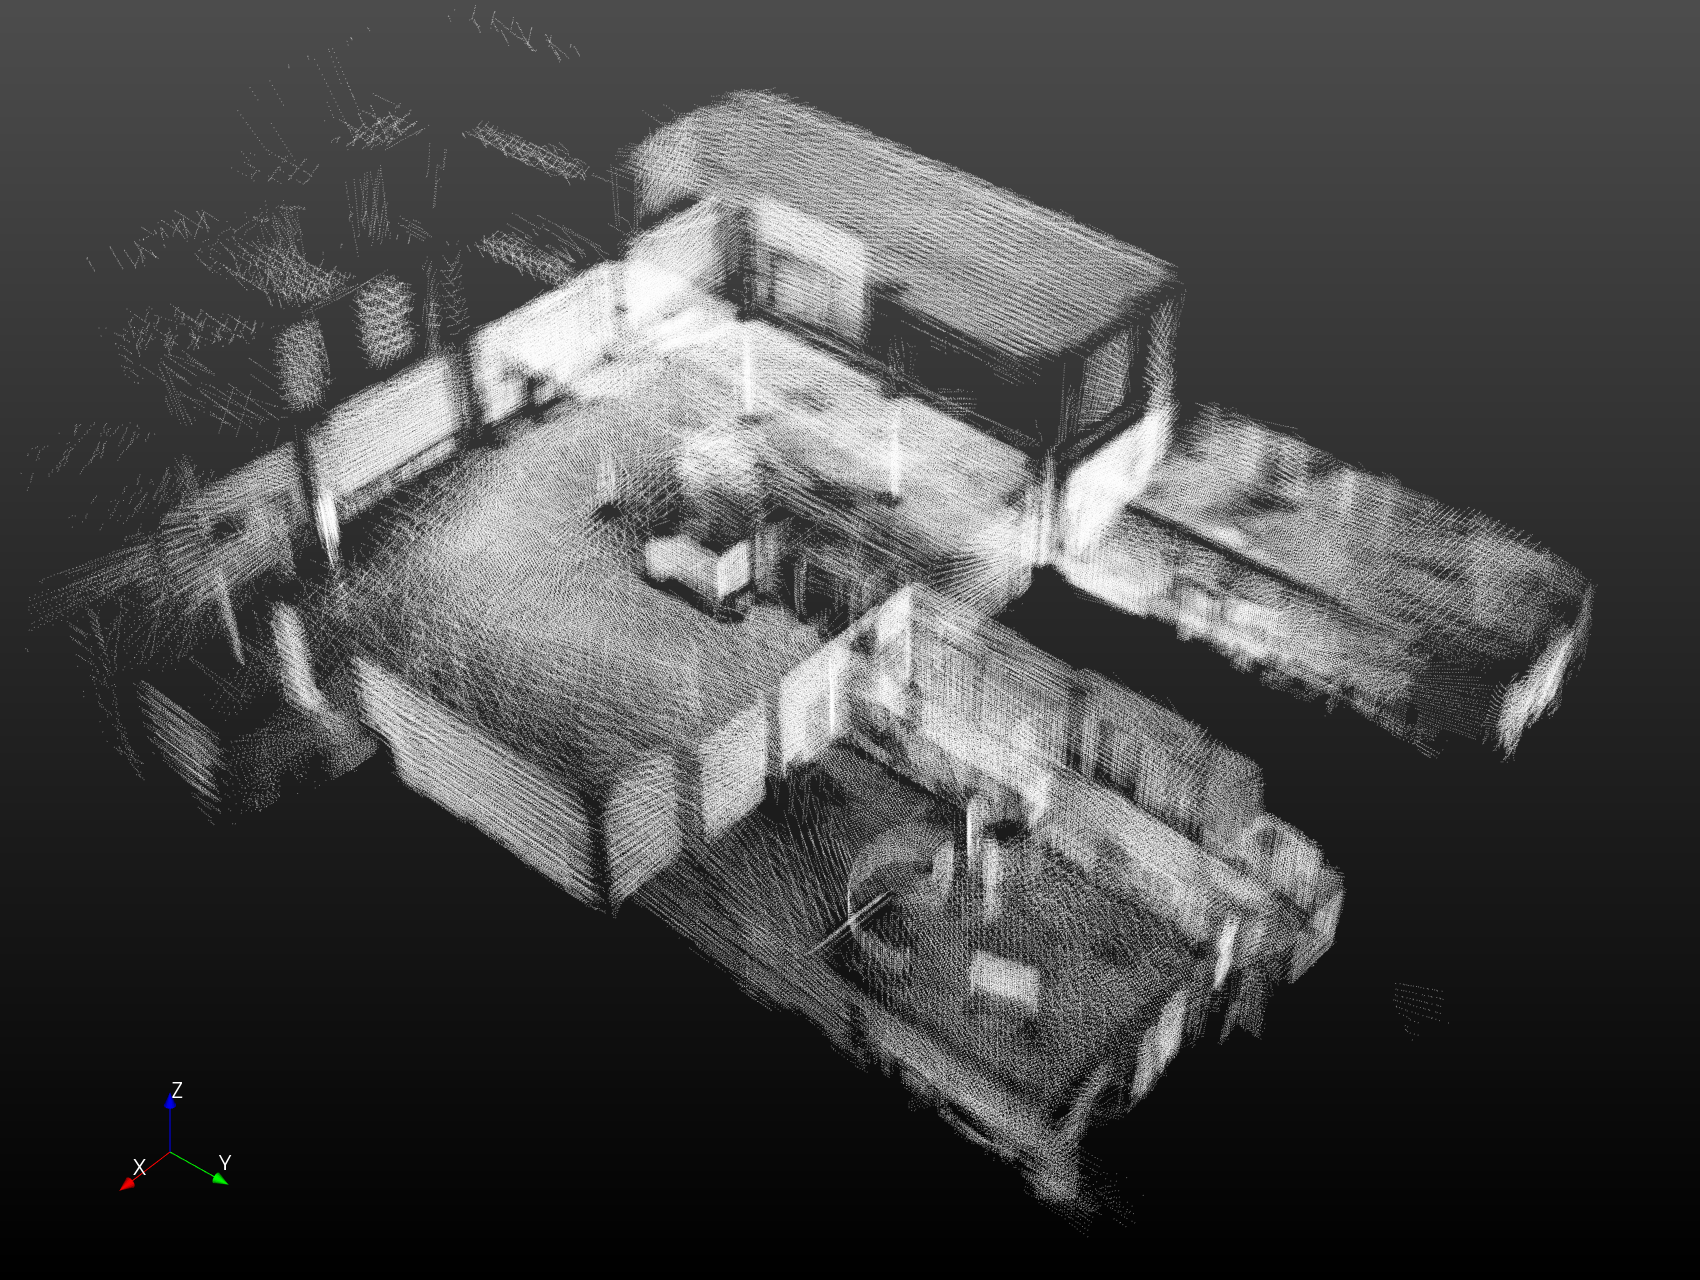
\includegraphics[width = 0.3\linewidth]{Maps1/PTCL2}} &
\subfloat{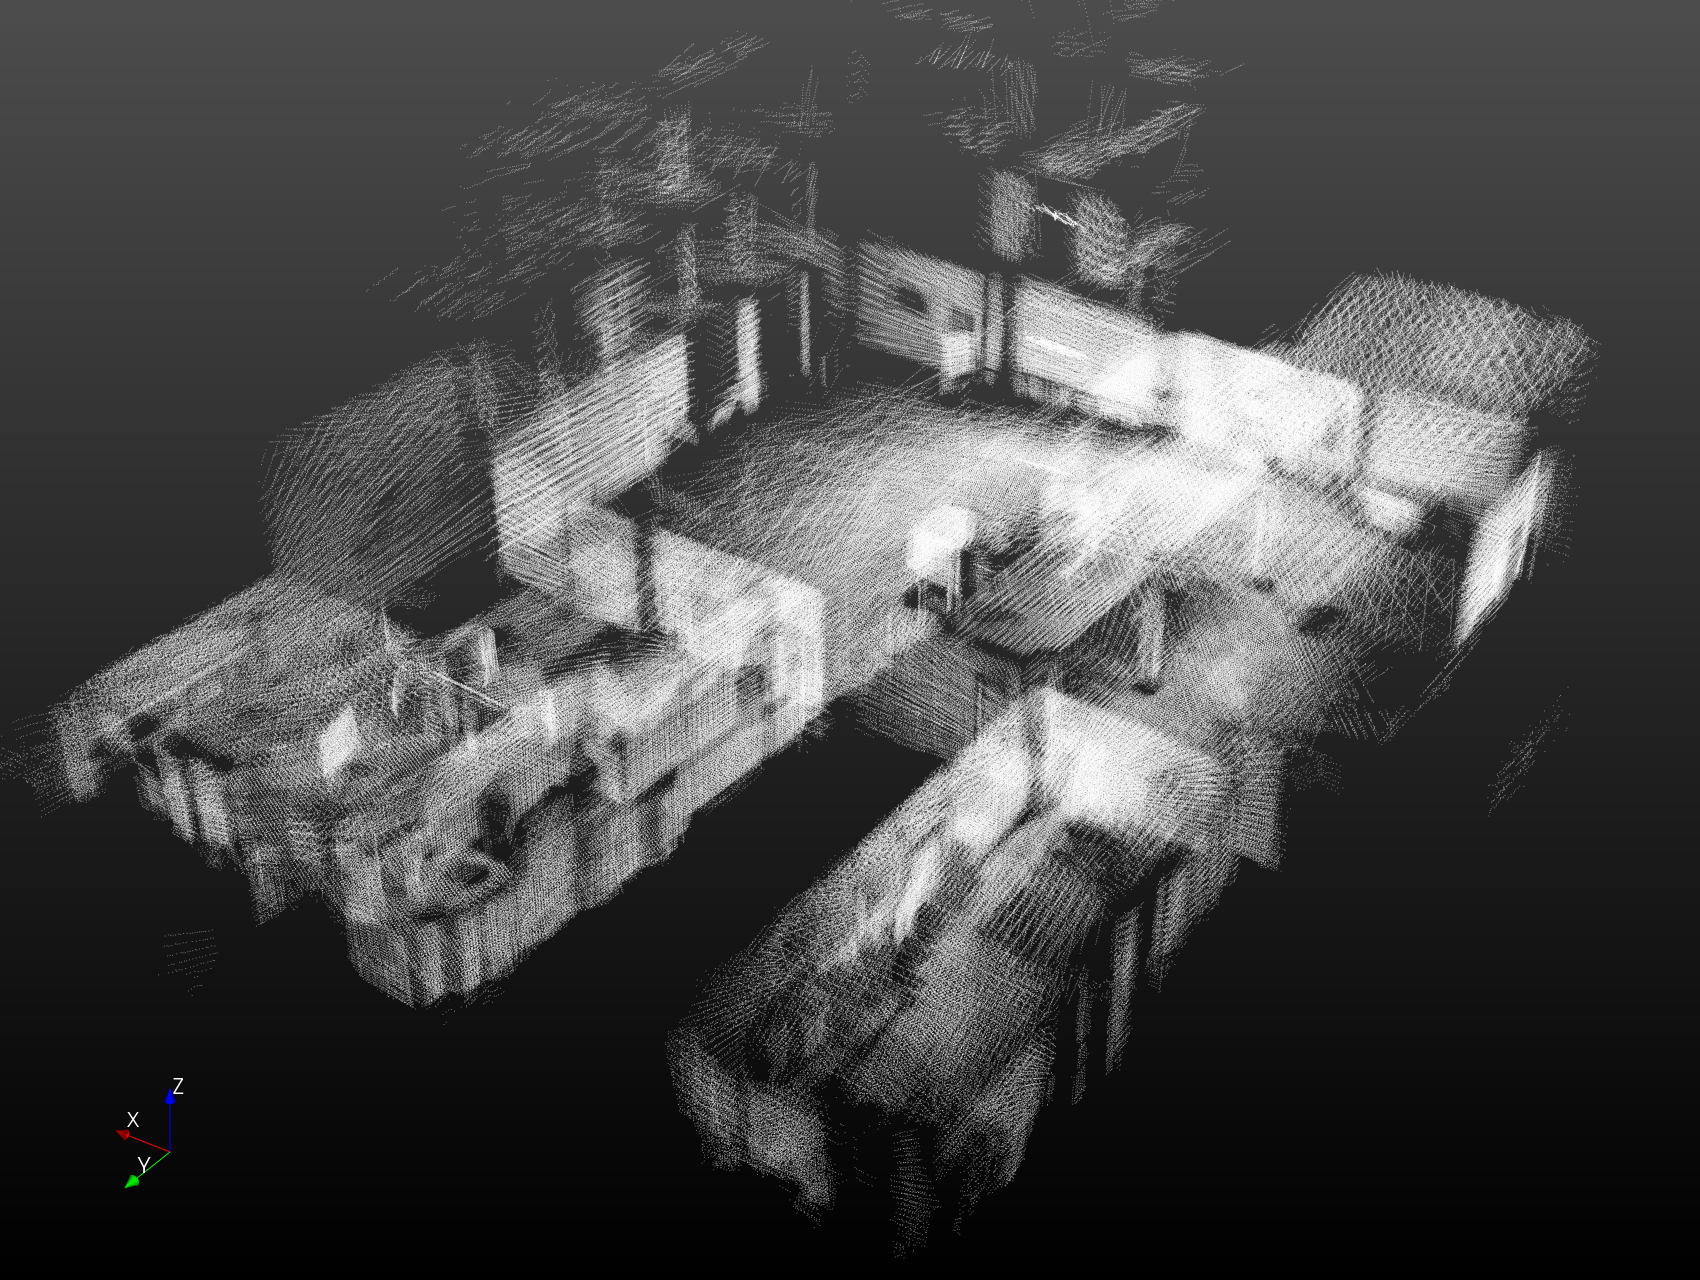
\includegraphics[width = 0.3\linewidth]{Maps1/PTCL3}} \\
\subfloat{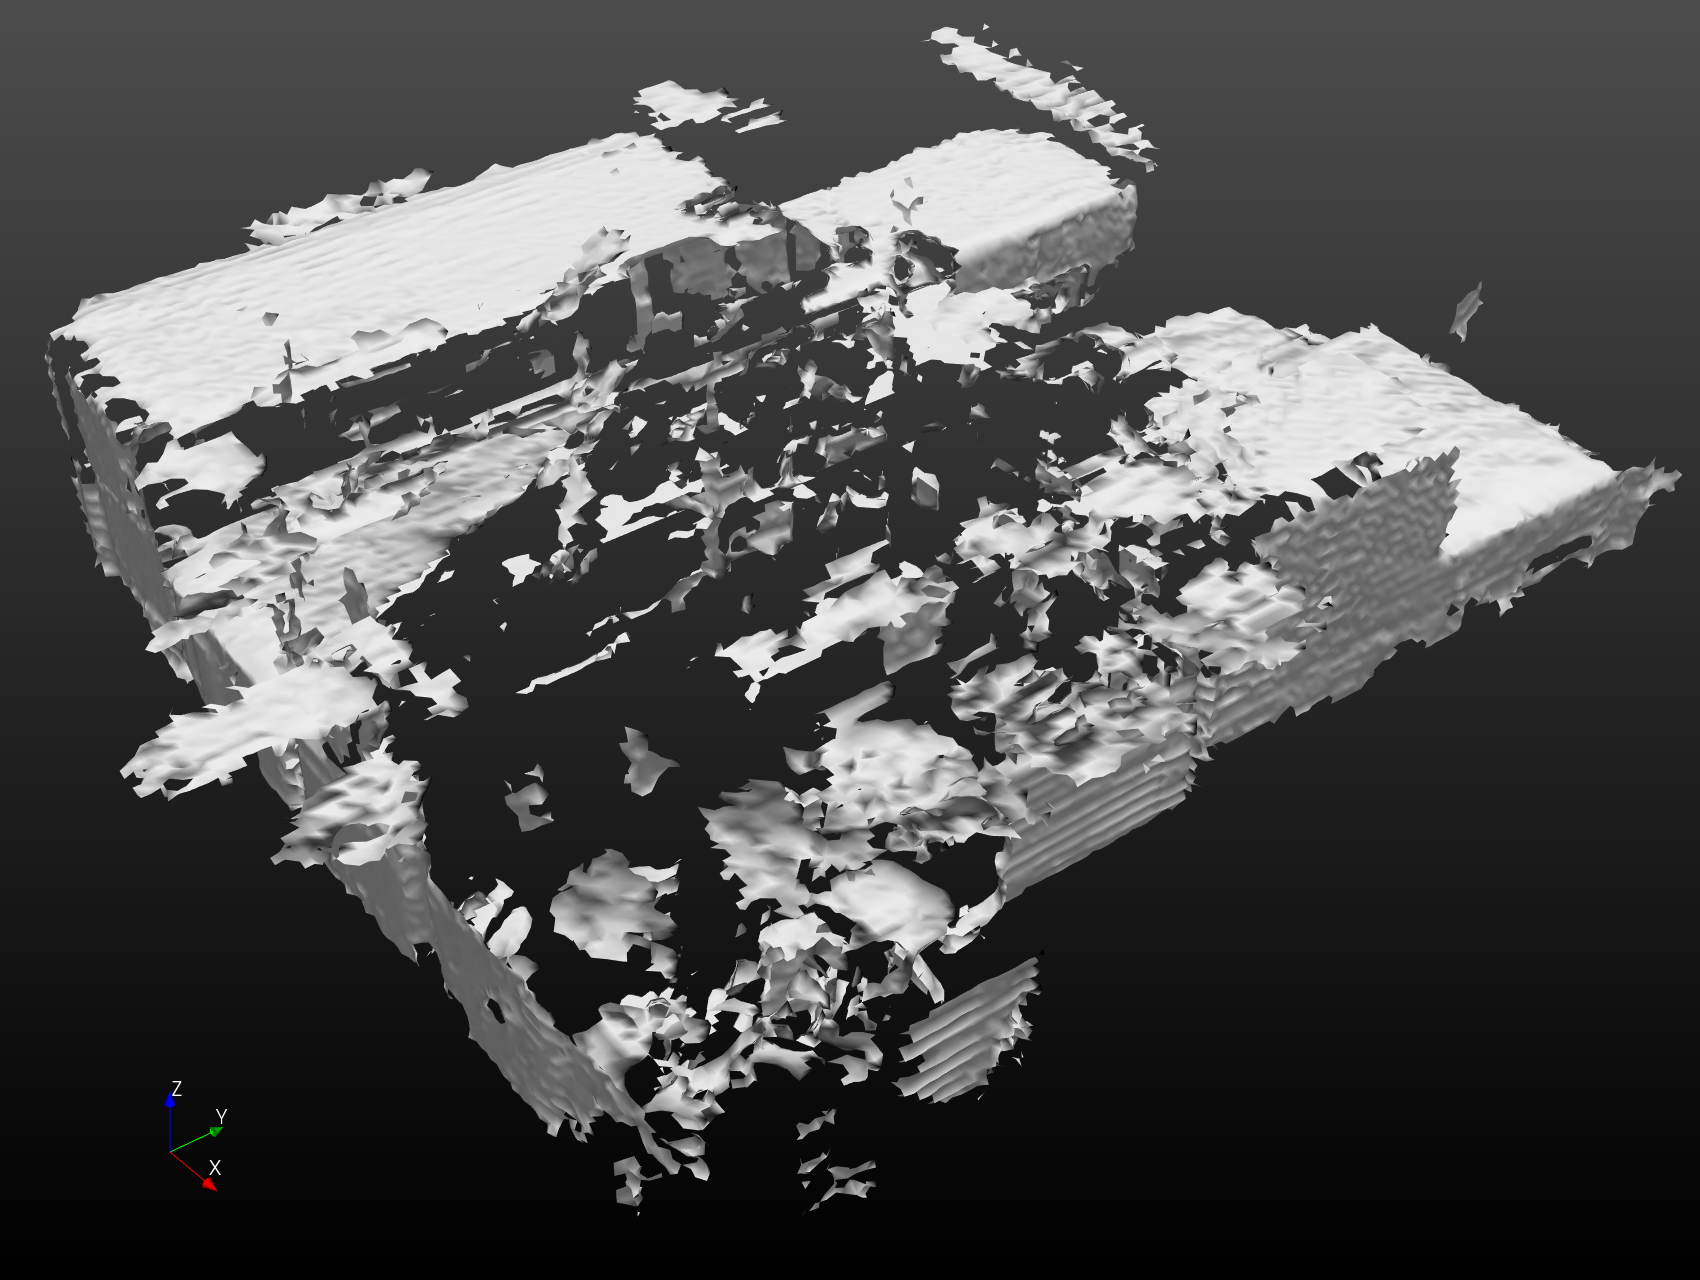
\includegraphics[width = 0.3\linewidth]{Maps1/Rec1}} &
\subfloat{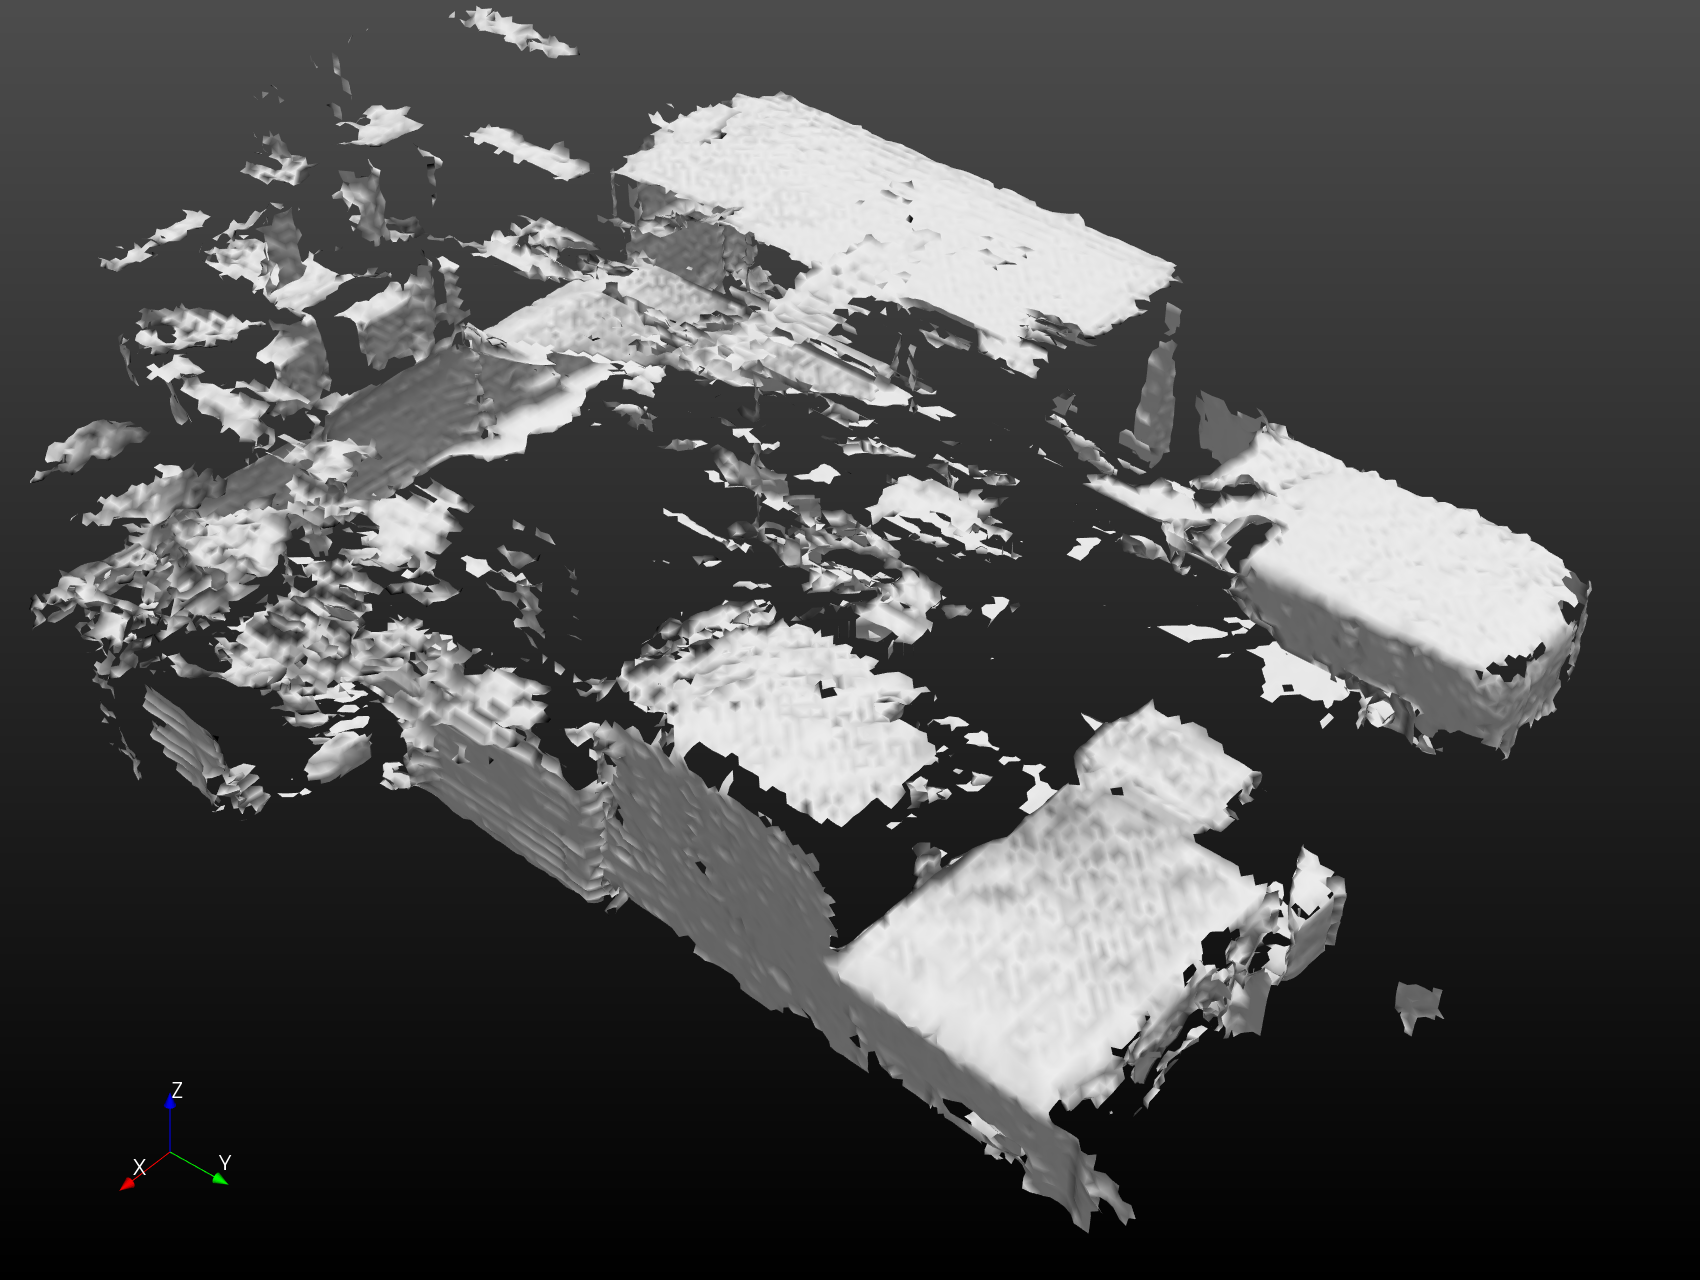
\includegraphics[width = 0.3\linewidth]{Maps1/Rec2}} &
\subfloat{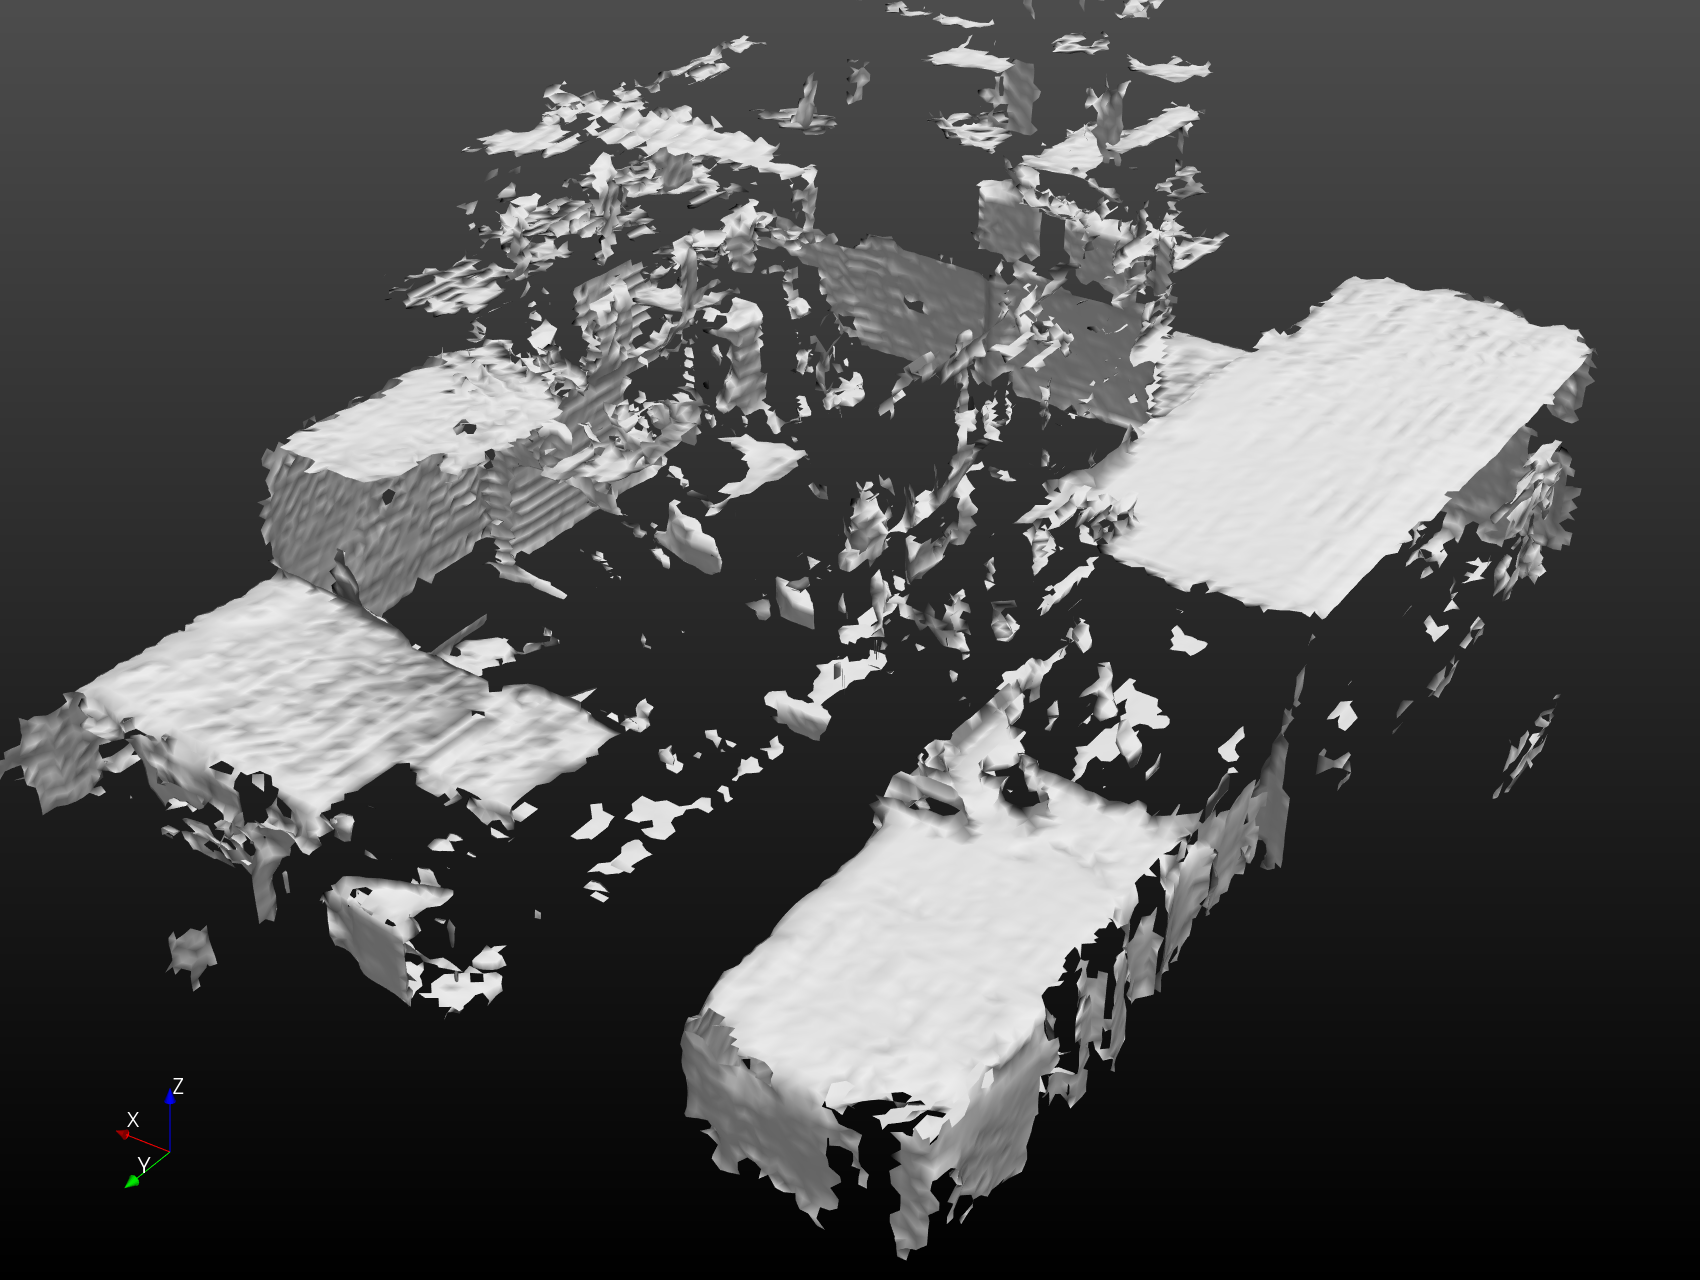
\includegraphics[width = 0.3\linewidth]{Maps1/Rec3}} \\
\subfloat{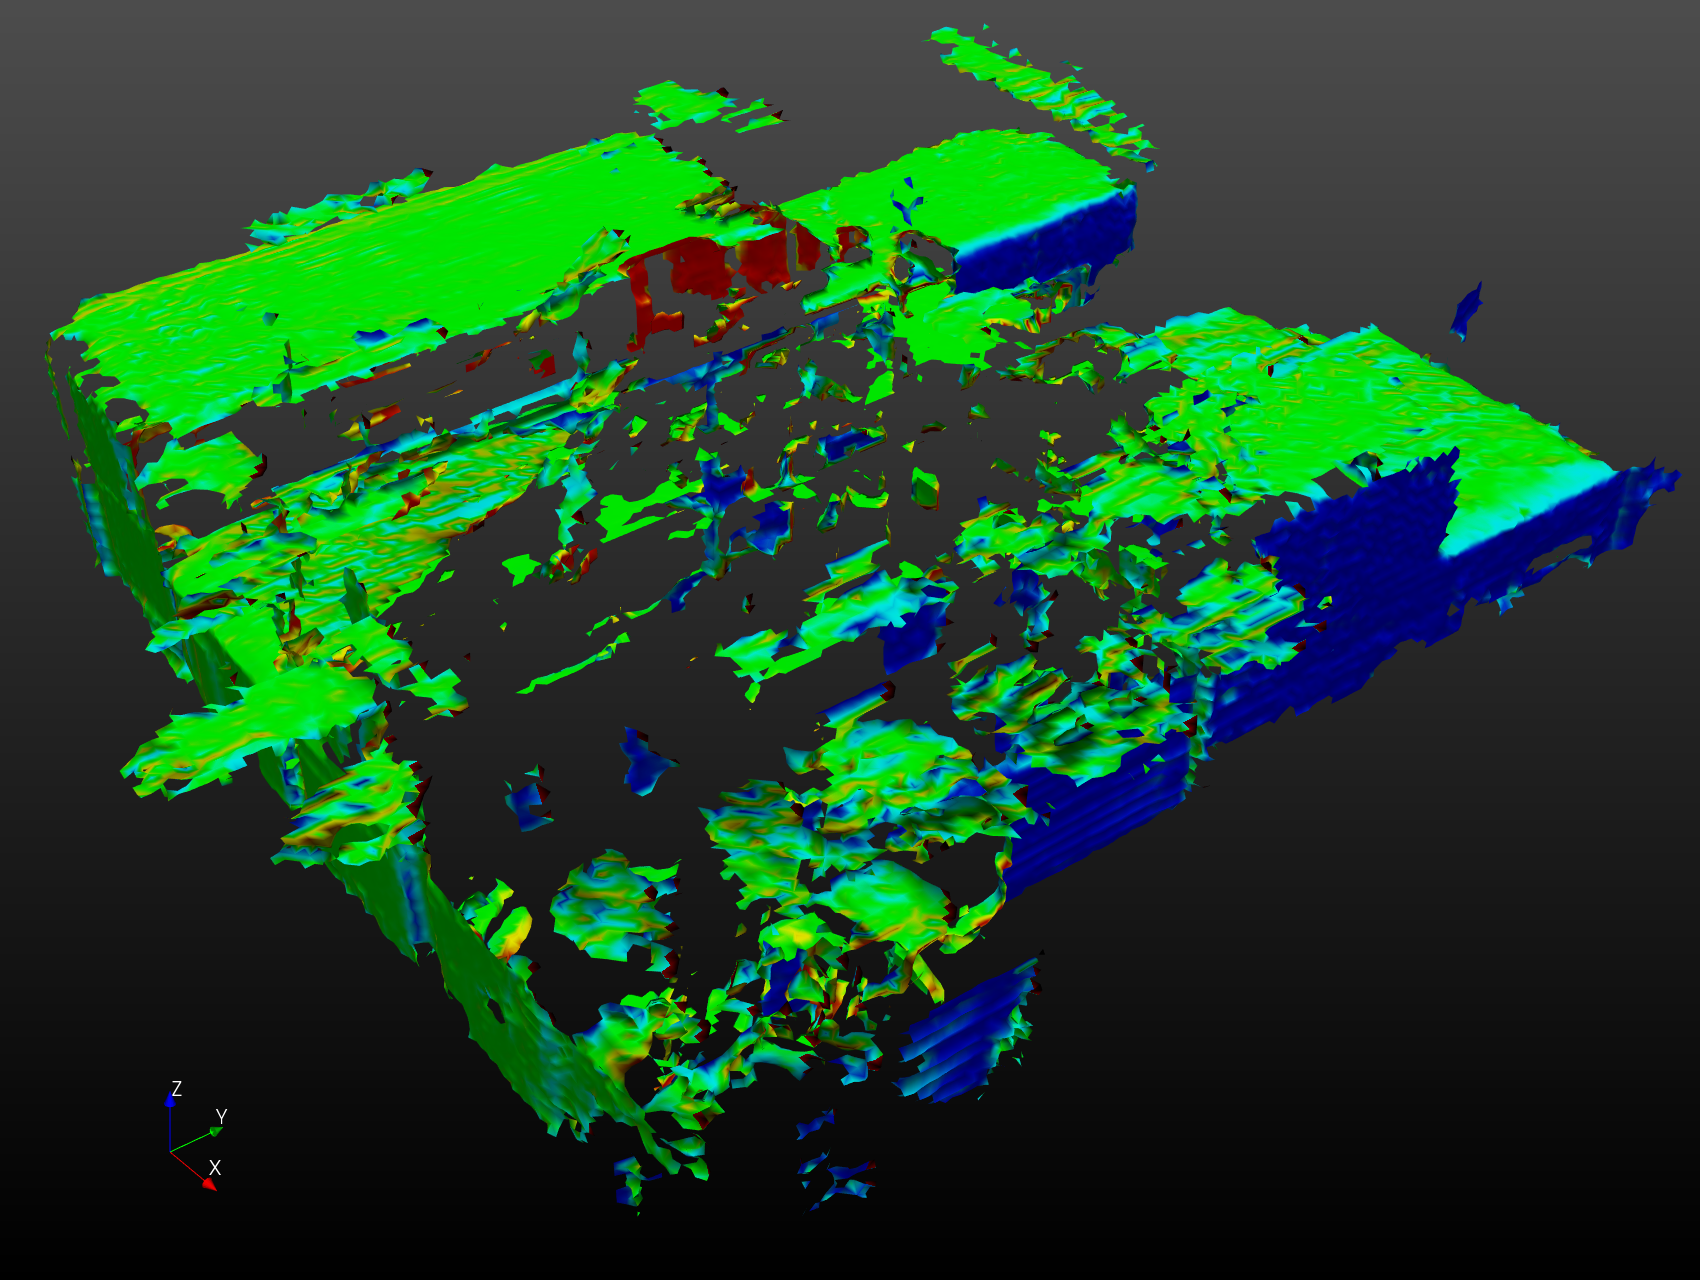
\includegraphics[width = 0.3\linewidth]{Maps1/Rec1N}} &
\subfloat{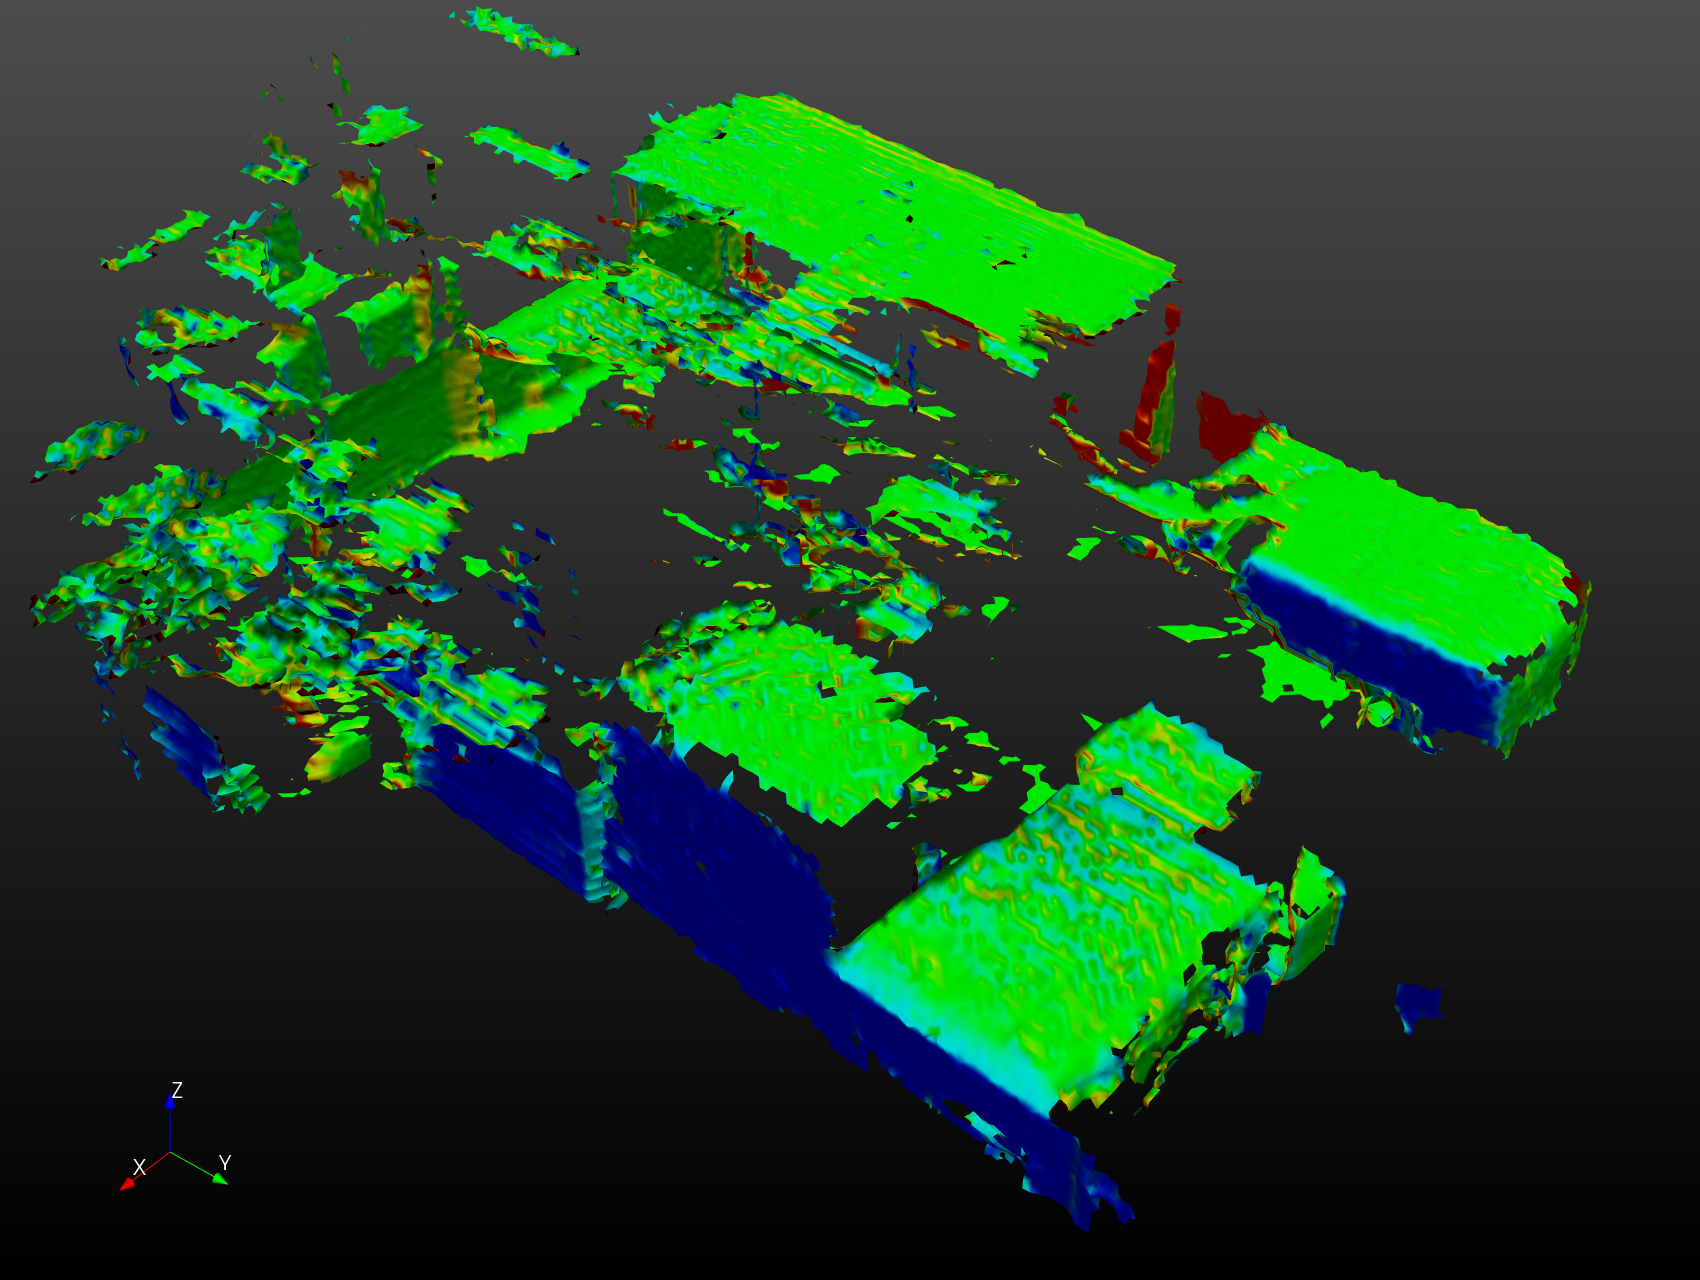
\includegraphics[width = 0.3\linewidth]{Maps1/Rec2N}} &
\subfloat{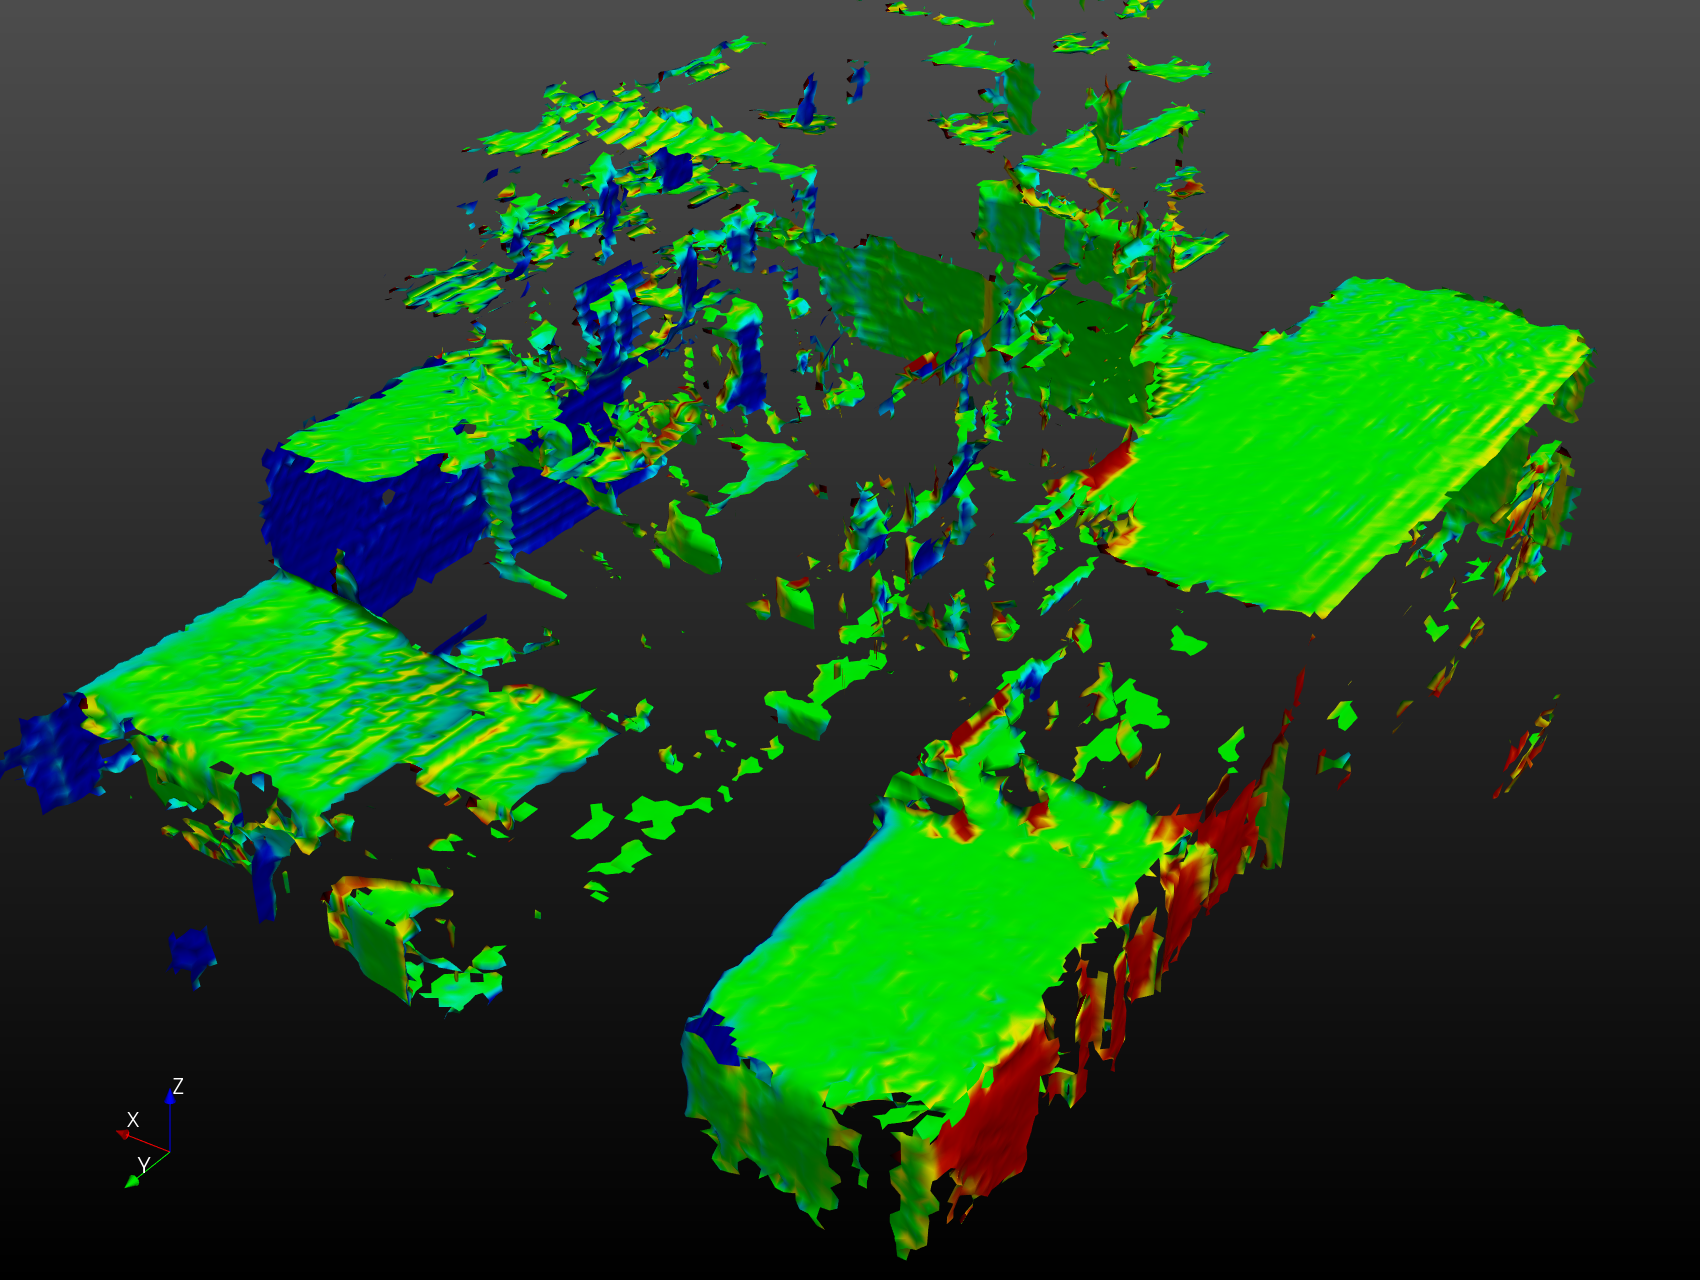
\includegraphics[width = 0.3\linewidth]{Maps1/Rec3N}} \\
\subfloat{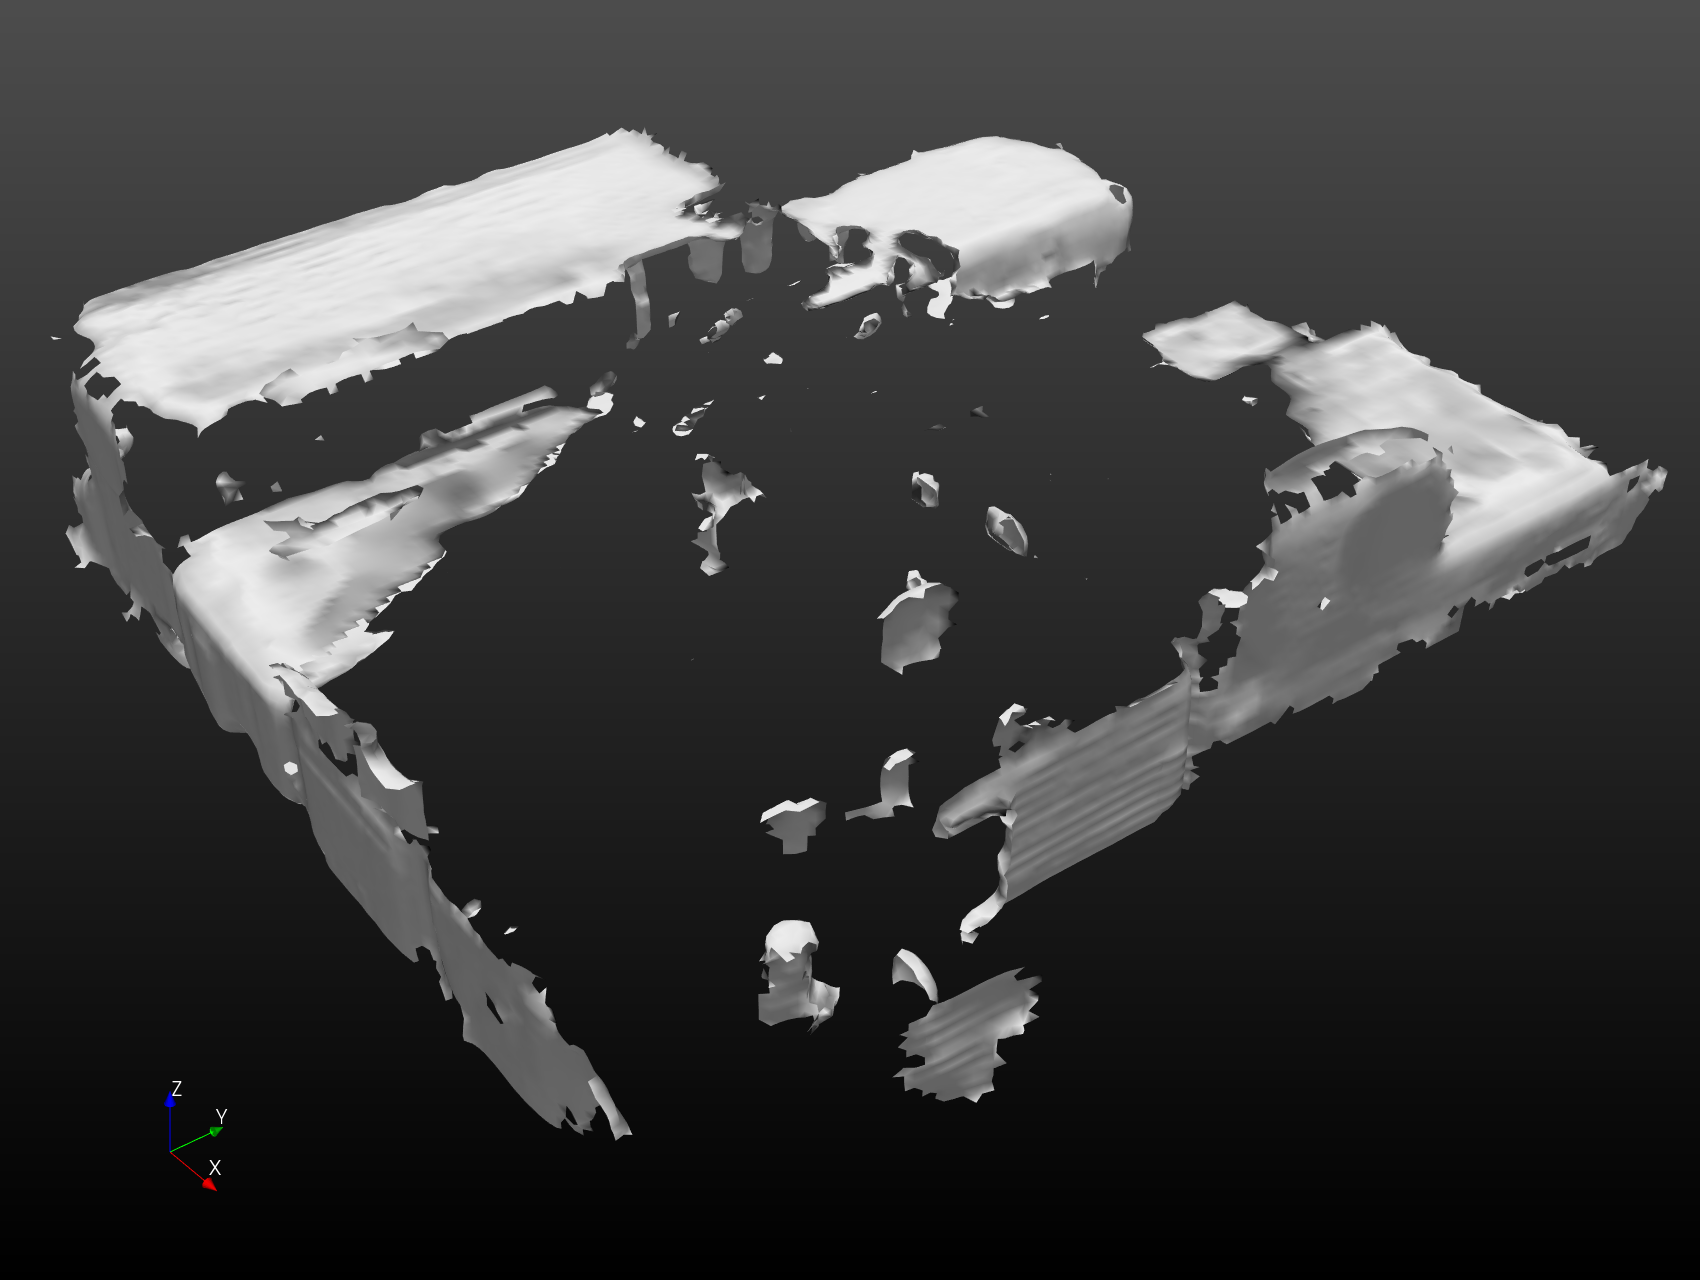
\includegraphics[width = 0.3\linewidth]{Maps1/RegRec1}} &
\subfloat{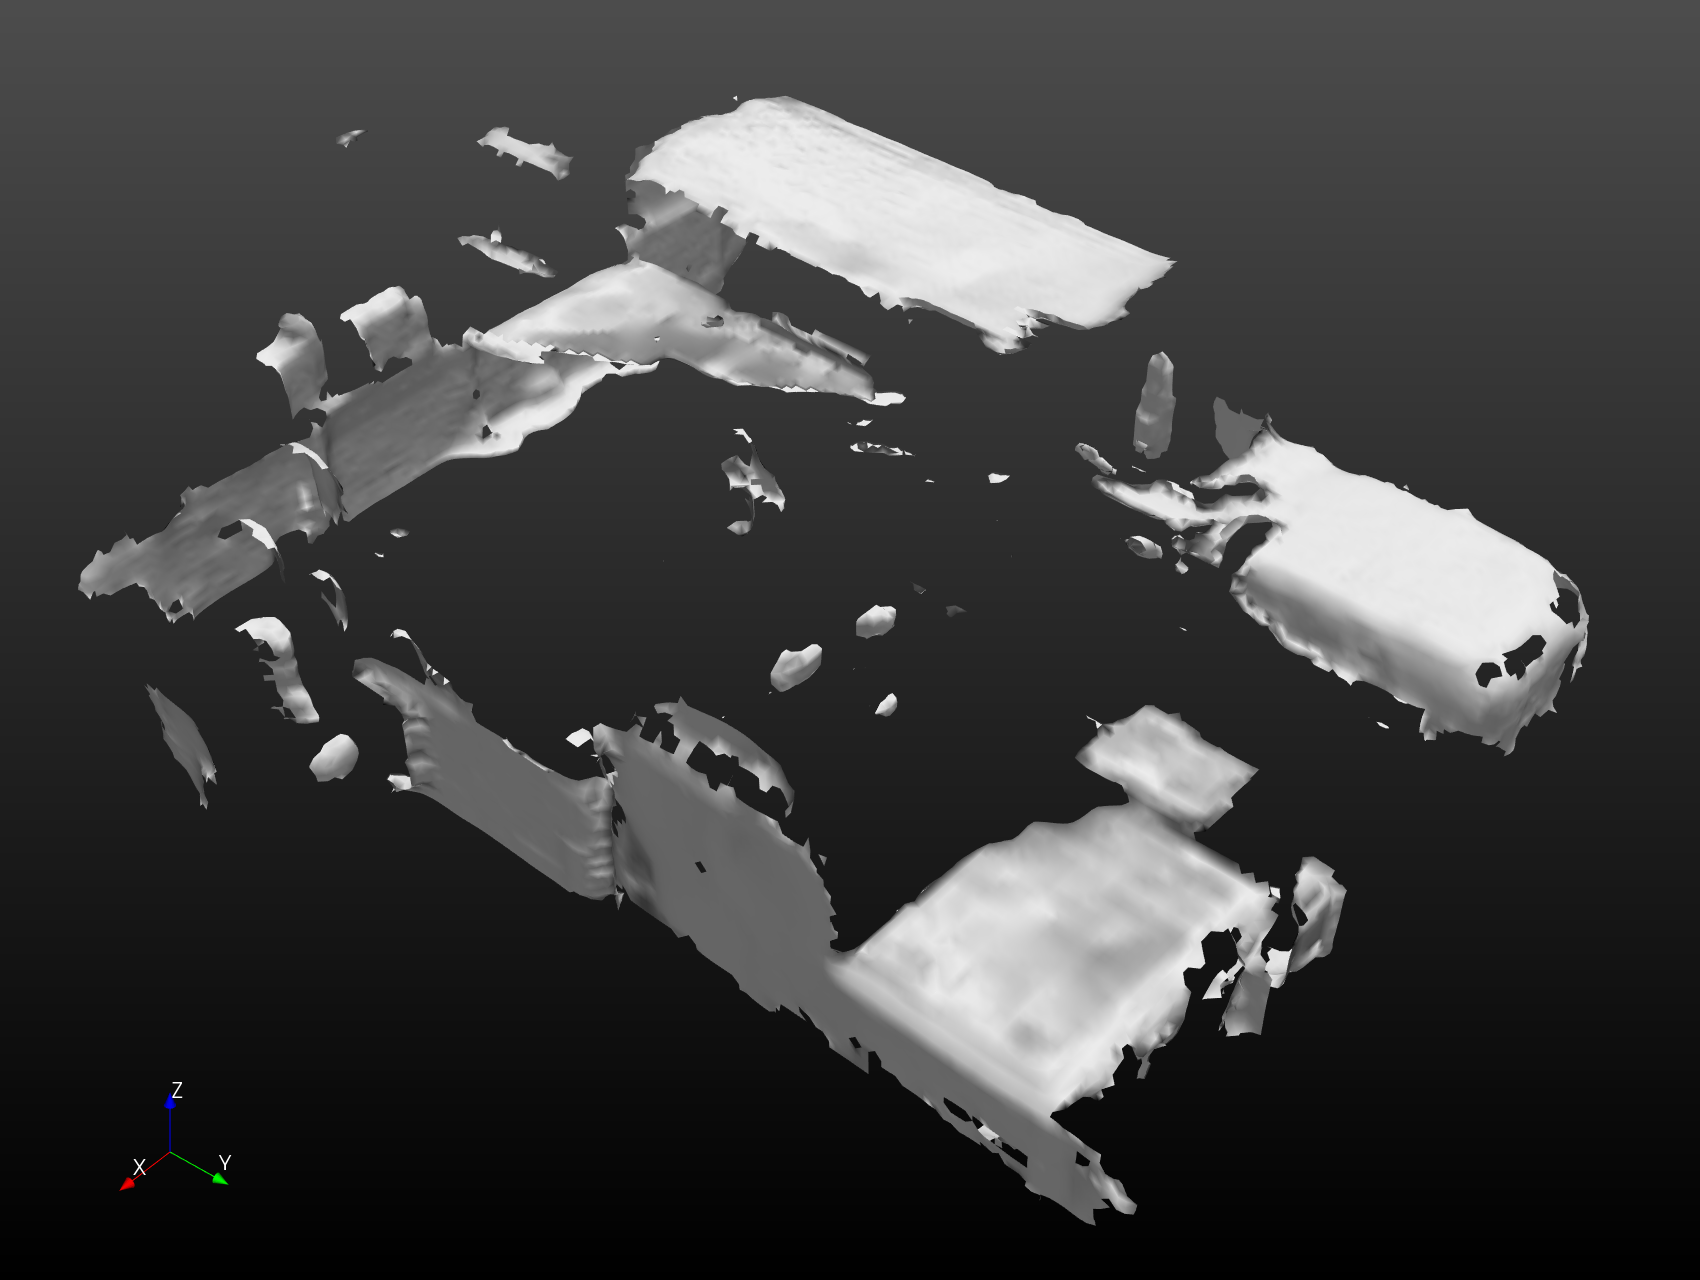
\includegraphics[width = 0.3\linewidth]{Maps1/RegRec2}} &
\subfloat{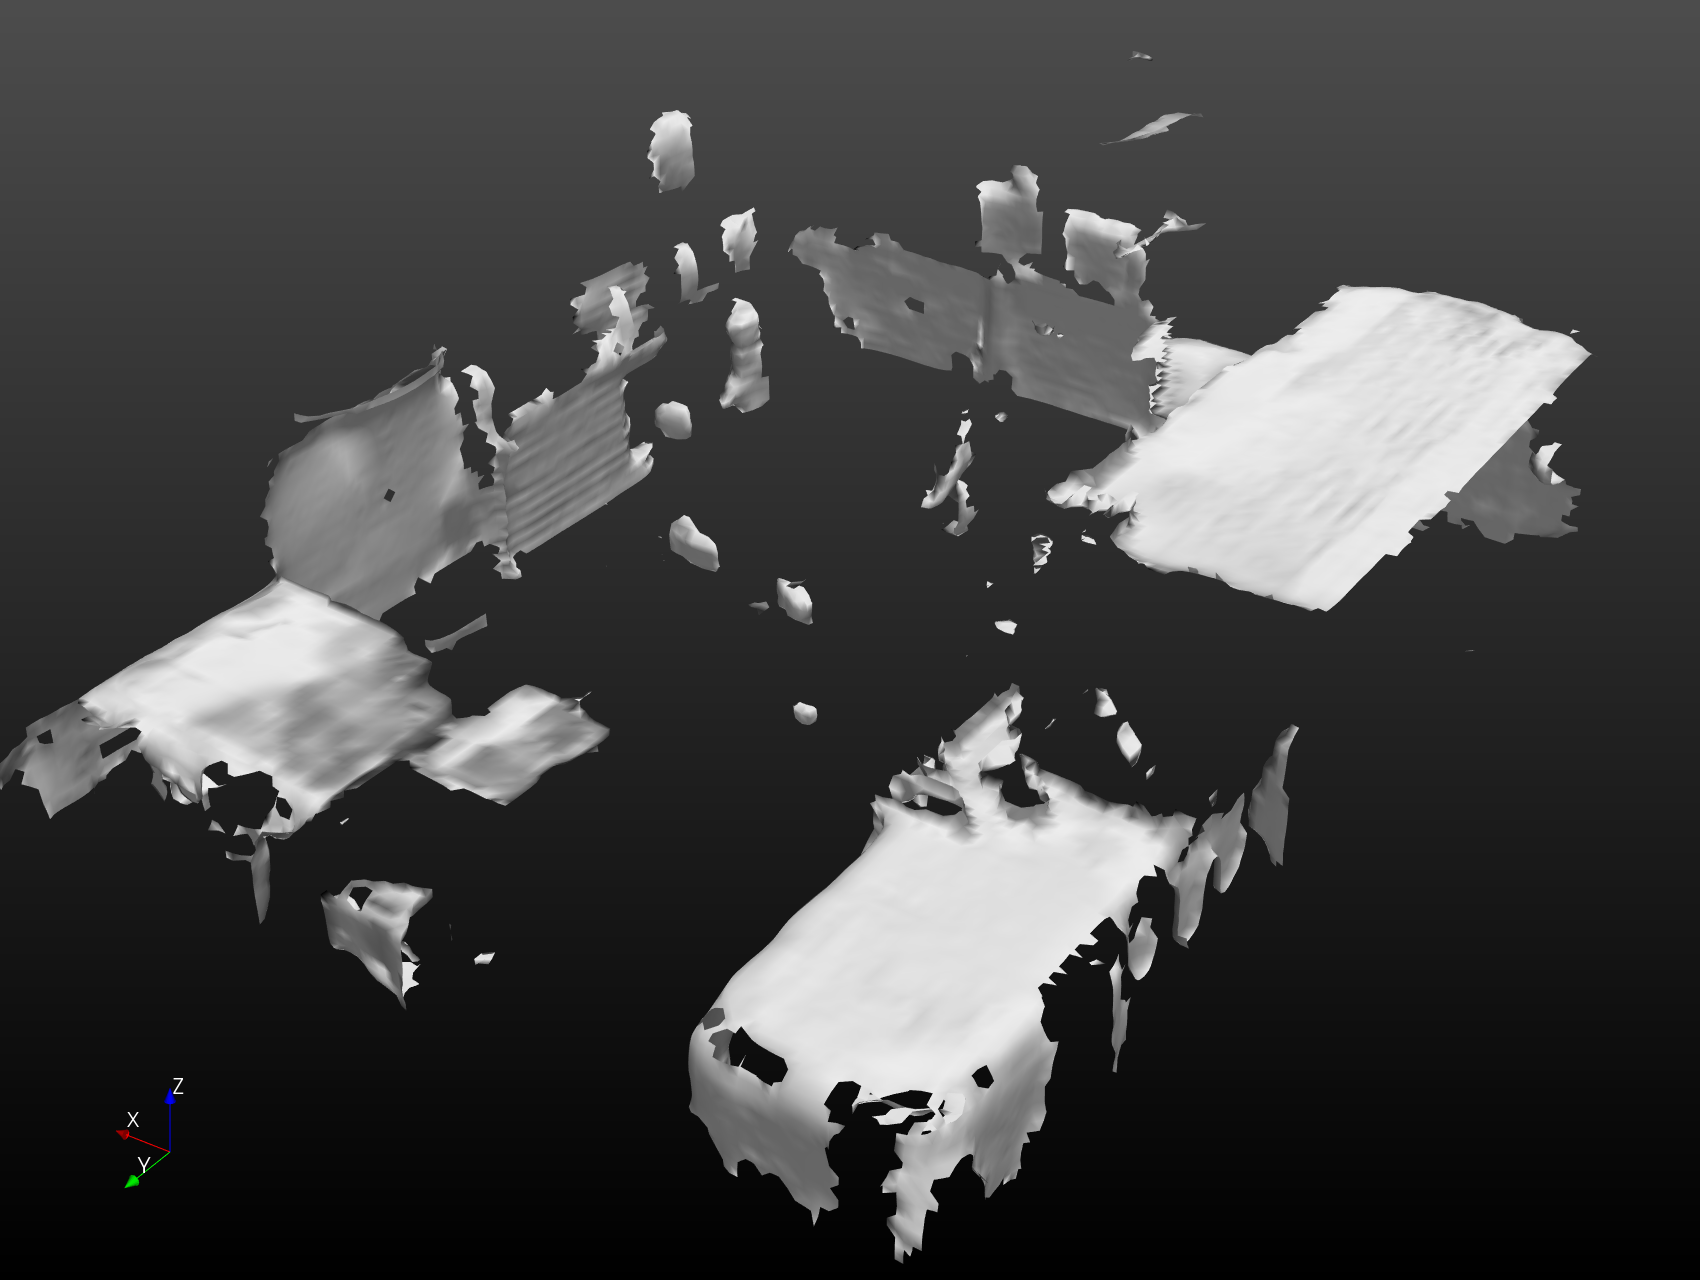
\includegraphics[width = 0.3\linewidth]{Maps1/RegRec3}}\\
\subfloat{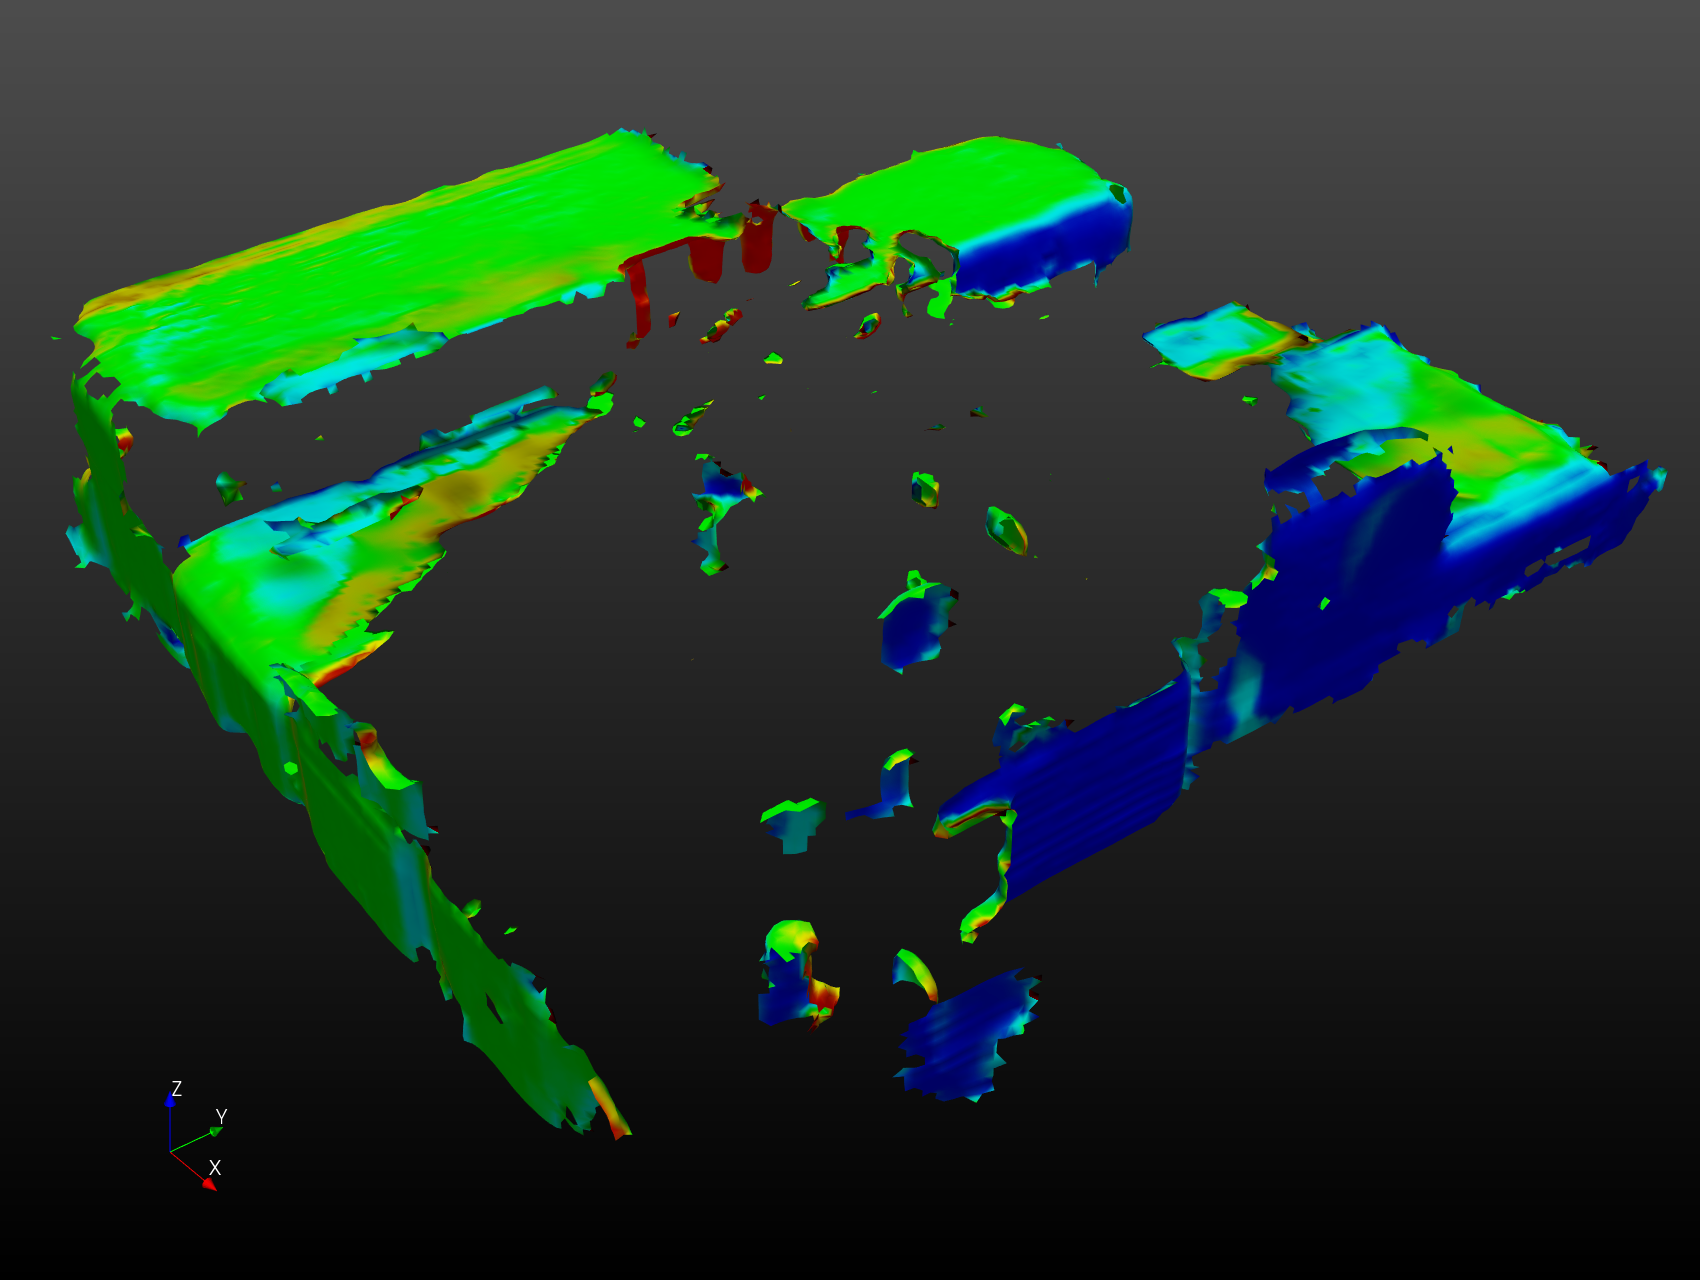
\includegraphics[width = 0.3\linewidth]{Maps1/RegRec1N}} &
\subfloat{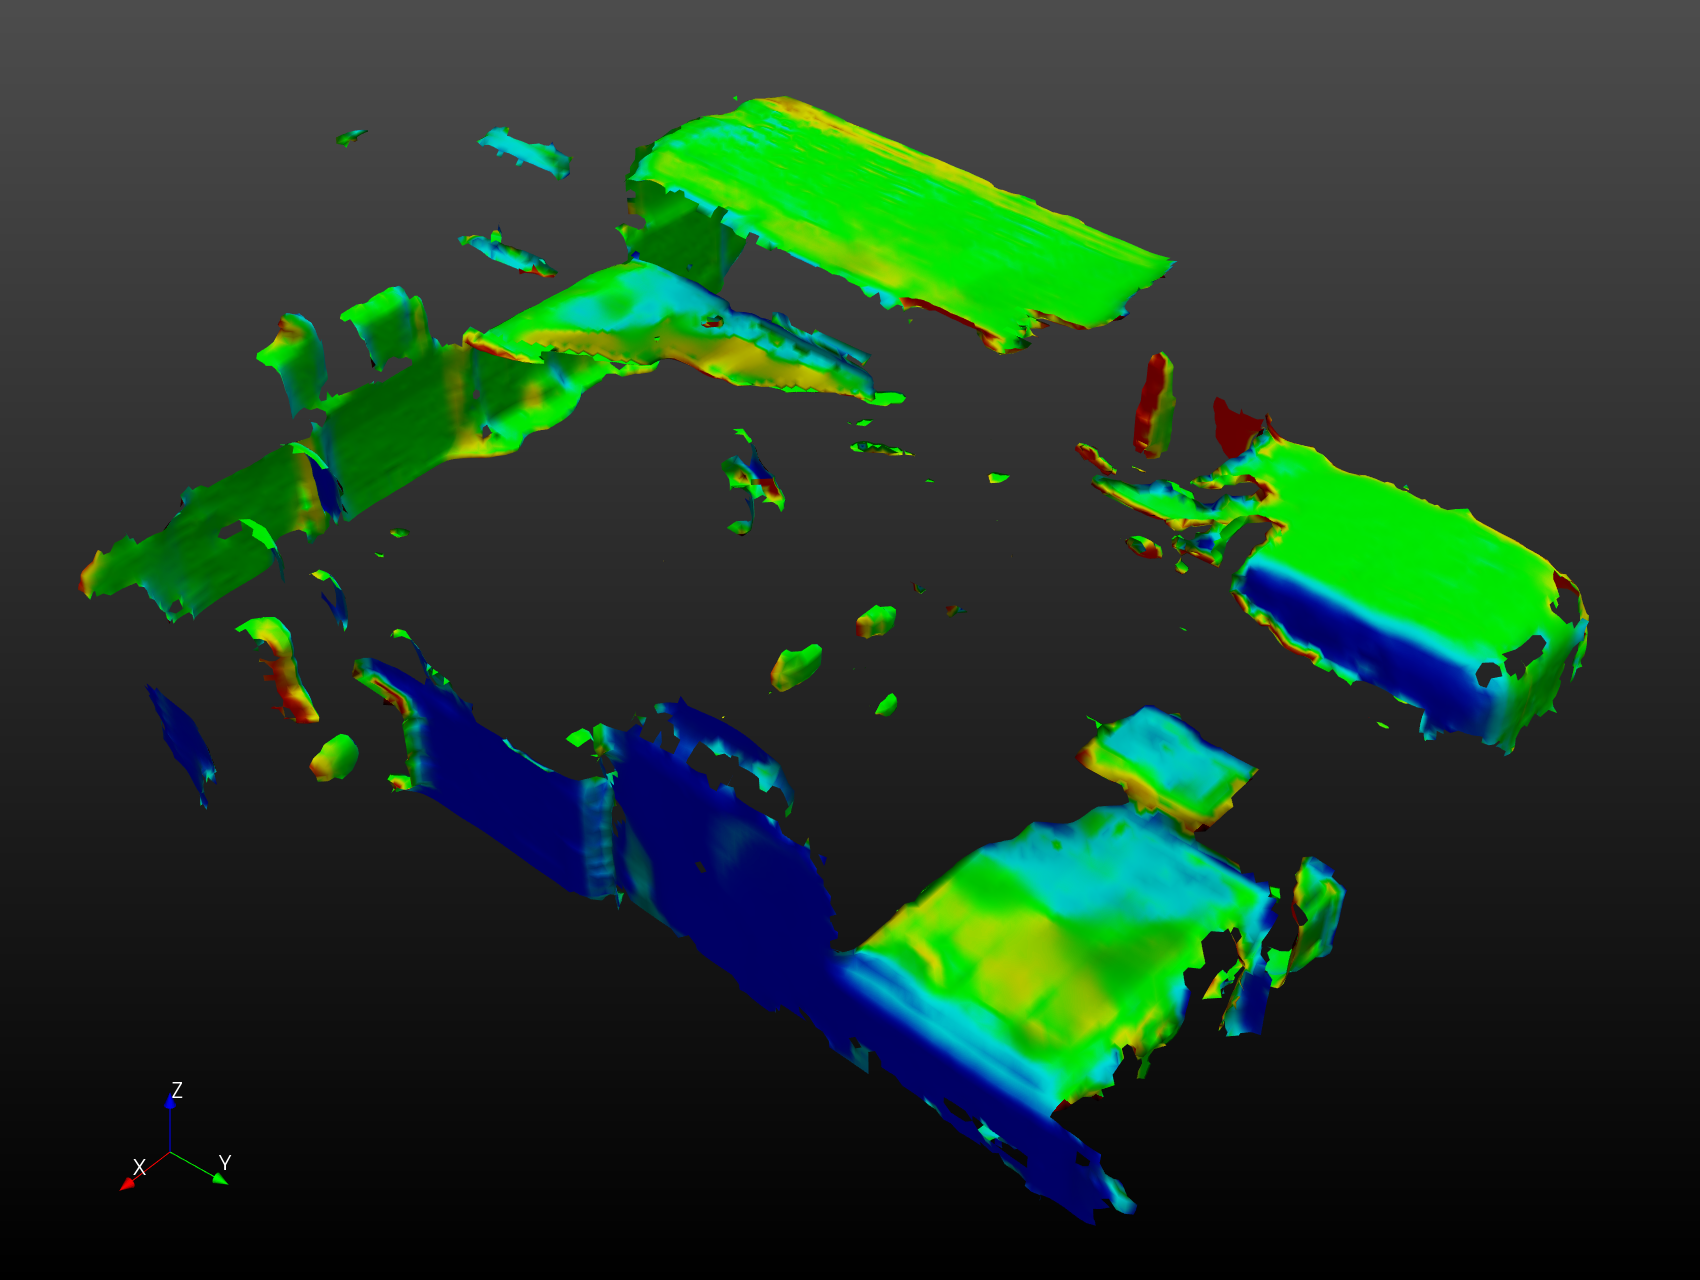
\includegraphics[width = 0.3\linewidth]{Maps1/RegRec2N}} &
\subfloat{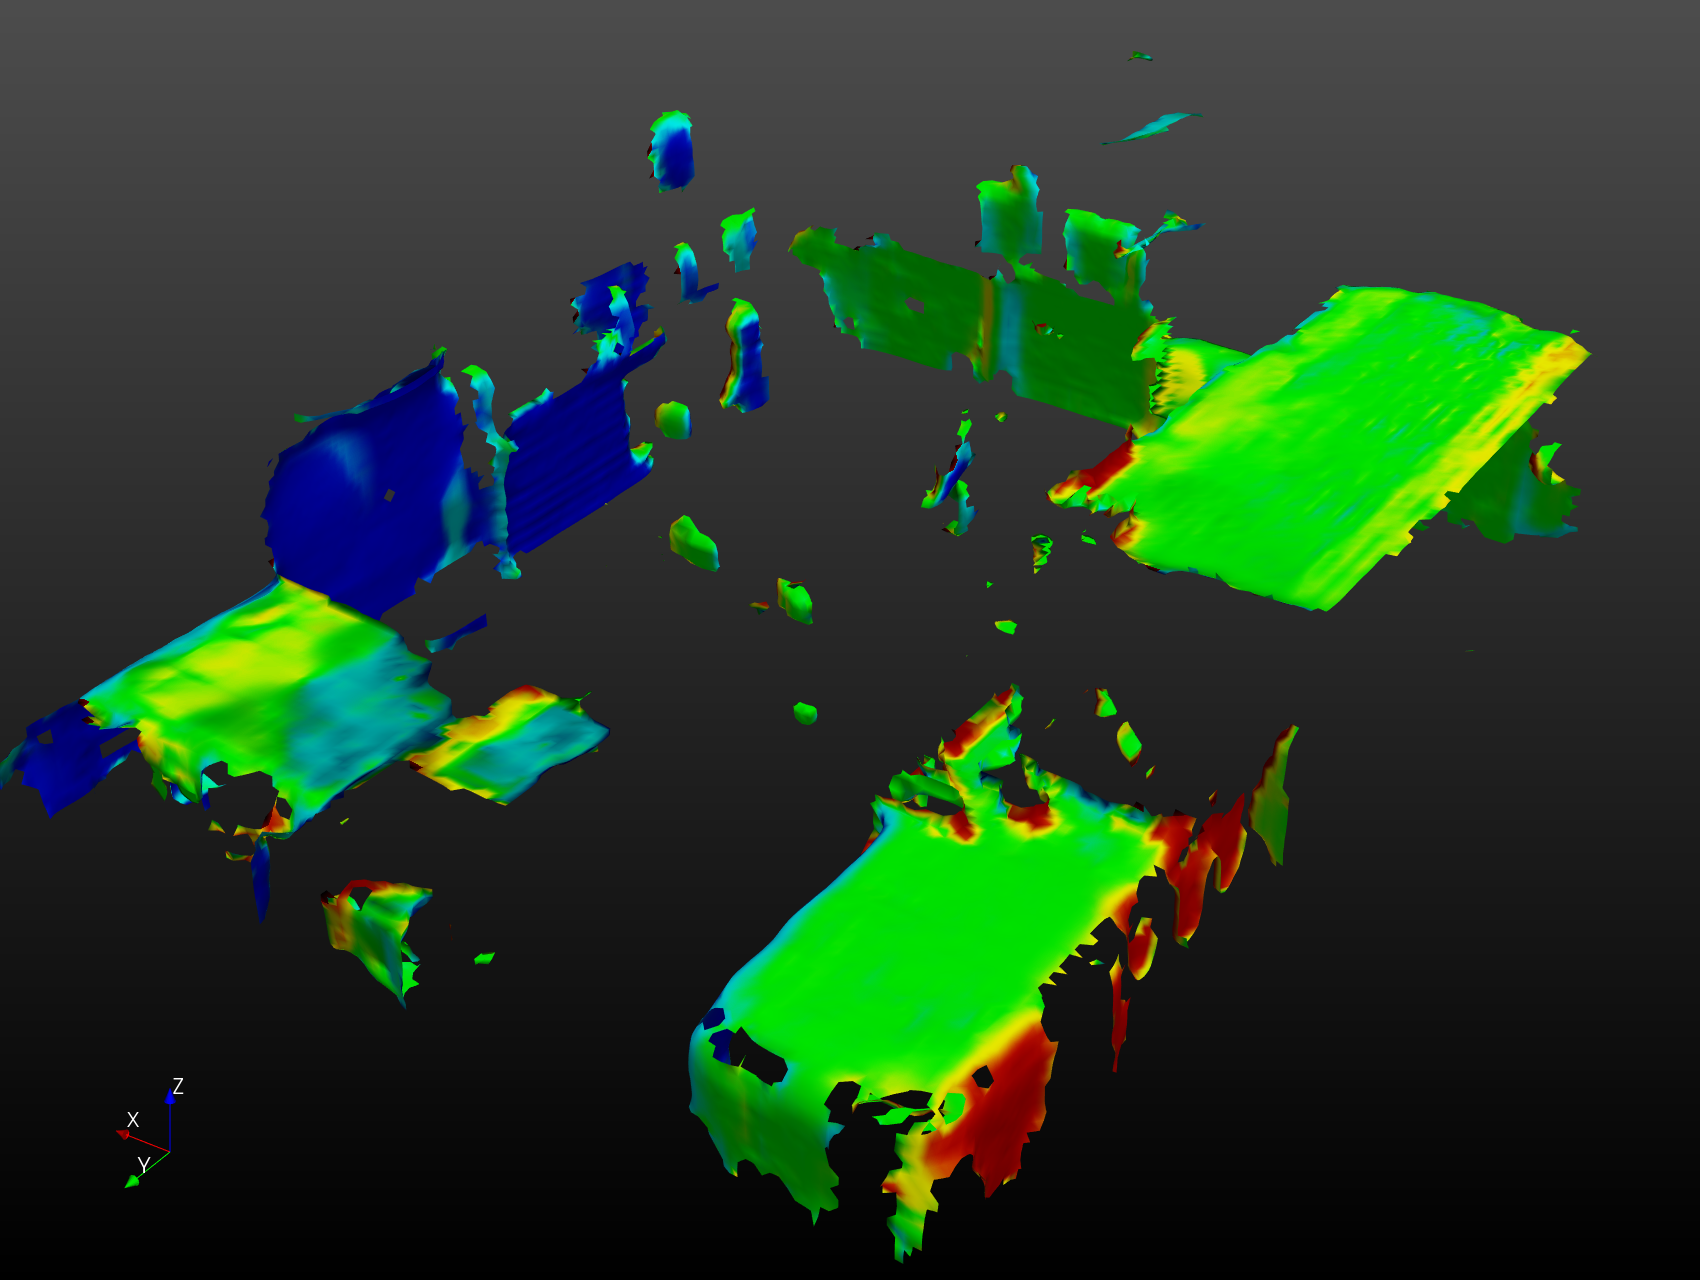
\includegraphics[width = 0.3\linewidth]{Maps1/RegRec3N}}
\end{tabular}
\caption{Results of running BORG CUBES to point clouds from first row. Second and third rows shows unregularized reconstruction (solid and normals coloured). Fourth and fifth rows show regularized reconstructions with $\lambda$ = 0.1 and 50 iterations (solid and normals coloured).}
\label{fig:EdinbDataset}
\end{figure}	
	
The second row and third rows show the point clouds after being input to the 3D reconstruction system. The results naturally depend on some hyperparameters, as explained in Section \ref{sec:Borg}. This figure shows results for edge-length equals to 0.2m and fusion threshold equals to 3. It can be seen that the surfaces are generally rough and noisy, due to imperfections in the laser scan data and in the inaccuracies associated with the SLAM solution.
	
The fourth and fifth rows show the result of regularizing the system using a $\lambda$ factor of 0.1 and number of iterations equals to 50. It is clear that by doing these, a lot of unconnected surfaces were removed, which was interpreted as noisy measurements for its high variational component. The surfaces that remain are mainly long connected walls and roofs, which are significantly smoother than the unregularized reconstruction. It can also be seen that some of the corners were smoothed, which actually should be sharp corners. This is understandable since the TV regularizer penalizes high variational profile, which ends up smoothing corners.
		
	\subsection{Oxford's Information Engineering Building Dataset}
	
This dataset was collected specifically for this project. The sensor goes through 2 loops, travelling about 210 meters. It passes through 10 doors, one big room, and it can reach a height of 20 meters. It also contains static objects and moving people.
	
Since this dataset is more segmented than the Edinburgh dataset and the loops are performed in two different sections, it was more sensitive to the parameters set by the loop closure system. It is also noted that there are significantly more windows in the Information Engineering Building (IEB), and combined with the faster velocity of the sensor have made the point clouds less dense. 
	
In total, 160 point clouds were collected, with approximately 6000 points per point cloud. The full path of the sensor and the position of the loop closures can be seen in Figure \ref{fig:TopViewIEBDataset}.
	
In the figure, the numbers are labelling the different rooms that were explored during the experiment. The path taken was from 1-8, then 1-4, 9-11, then, 7, 8 and finally 1. Therefore, two big loops were made, which was convenient to test multiple loops in the environment. Loop closures were detected in the rooms expected (1-4, 7 and 8). This was a more challenging problem to tackle than the Edinburgh dataset. The reason for this is that the loops were made in longer distances, which means that the drift accumulated between them were higher, and thus it made it difficult to identify loops using the heuristics outlined in Section \ref{subs:LoopCl}. However, even in longer distances the system performed well and a relatively accurate map of the building could be generated. This map was then input to the 3D reconstruction system. 
	
\begin{figure}[h]
\centering
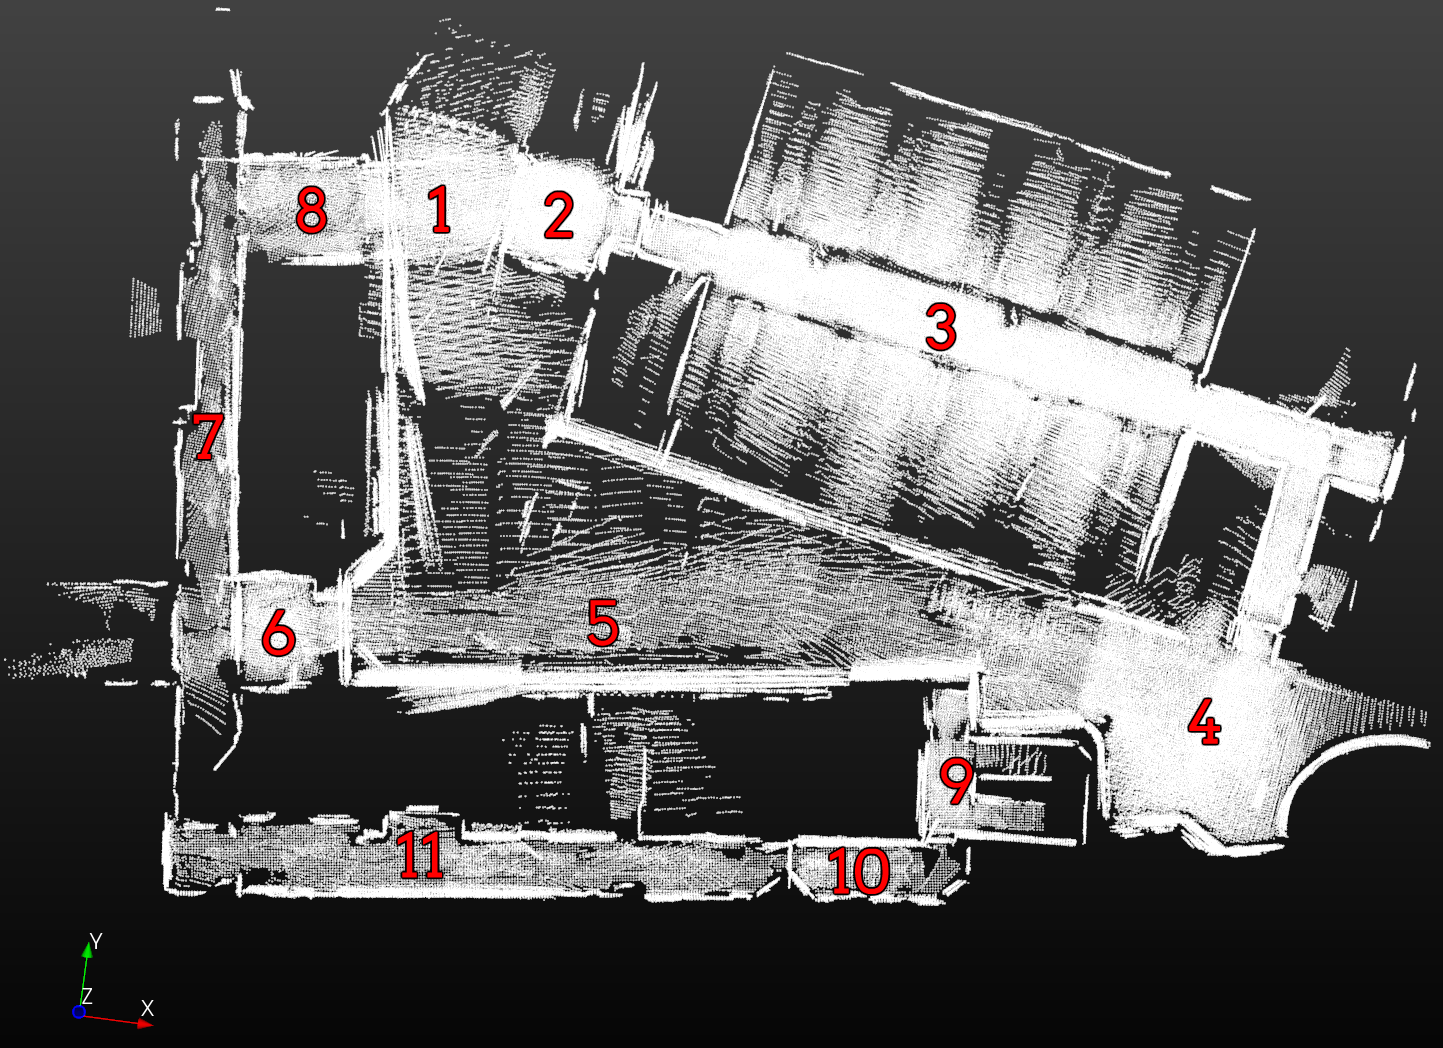
\includegraphics[width=0.8\linewidth]{Maps2/TopViewMarked}
\caption{Bird's Eye view of the map of the IEB Dataset. The path taken was 1, 2, 3, 4, 5, 6, 7, 8, 1, 2, 3, 4, 9, 10, 11, 7, 8, 1. Loop Closures were detected in rooms 1, 2, 3, 4, 7, 8.}
\label{fig:TopViewIEBDataset}
\end{figure}

The results of the 3D reconstructed model after the SLAM solution can be seen in Figure \ref{fig:IEBDataset}. The first row shows the raw point clouds. For this dataset, the assumption about sparsity in corners and in windows is also valid. It can be seen that the corners are sparser than walls and roofs.
	
\begin{figure}
\centering
\caption*{\textbf{Oxford's Information Engineering Dataset}}
\begin{tabular}{cccc}
\subfloat{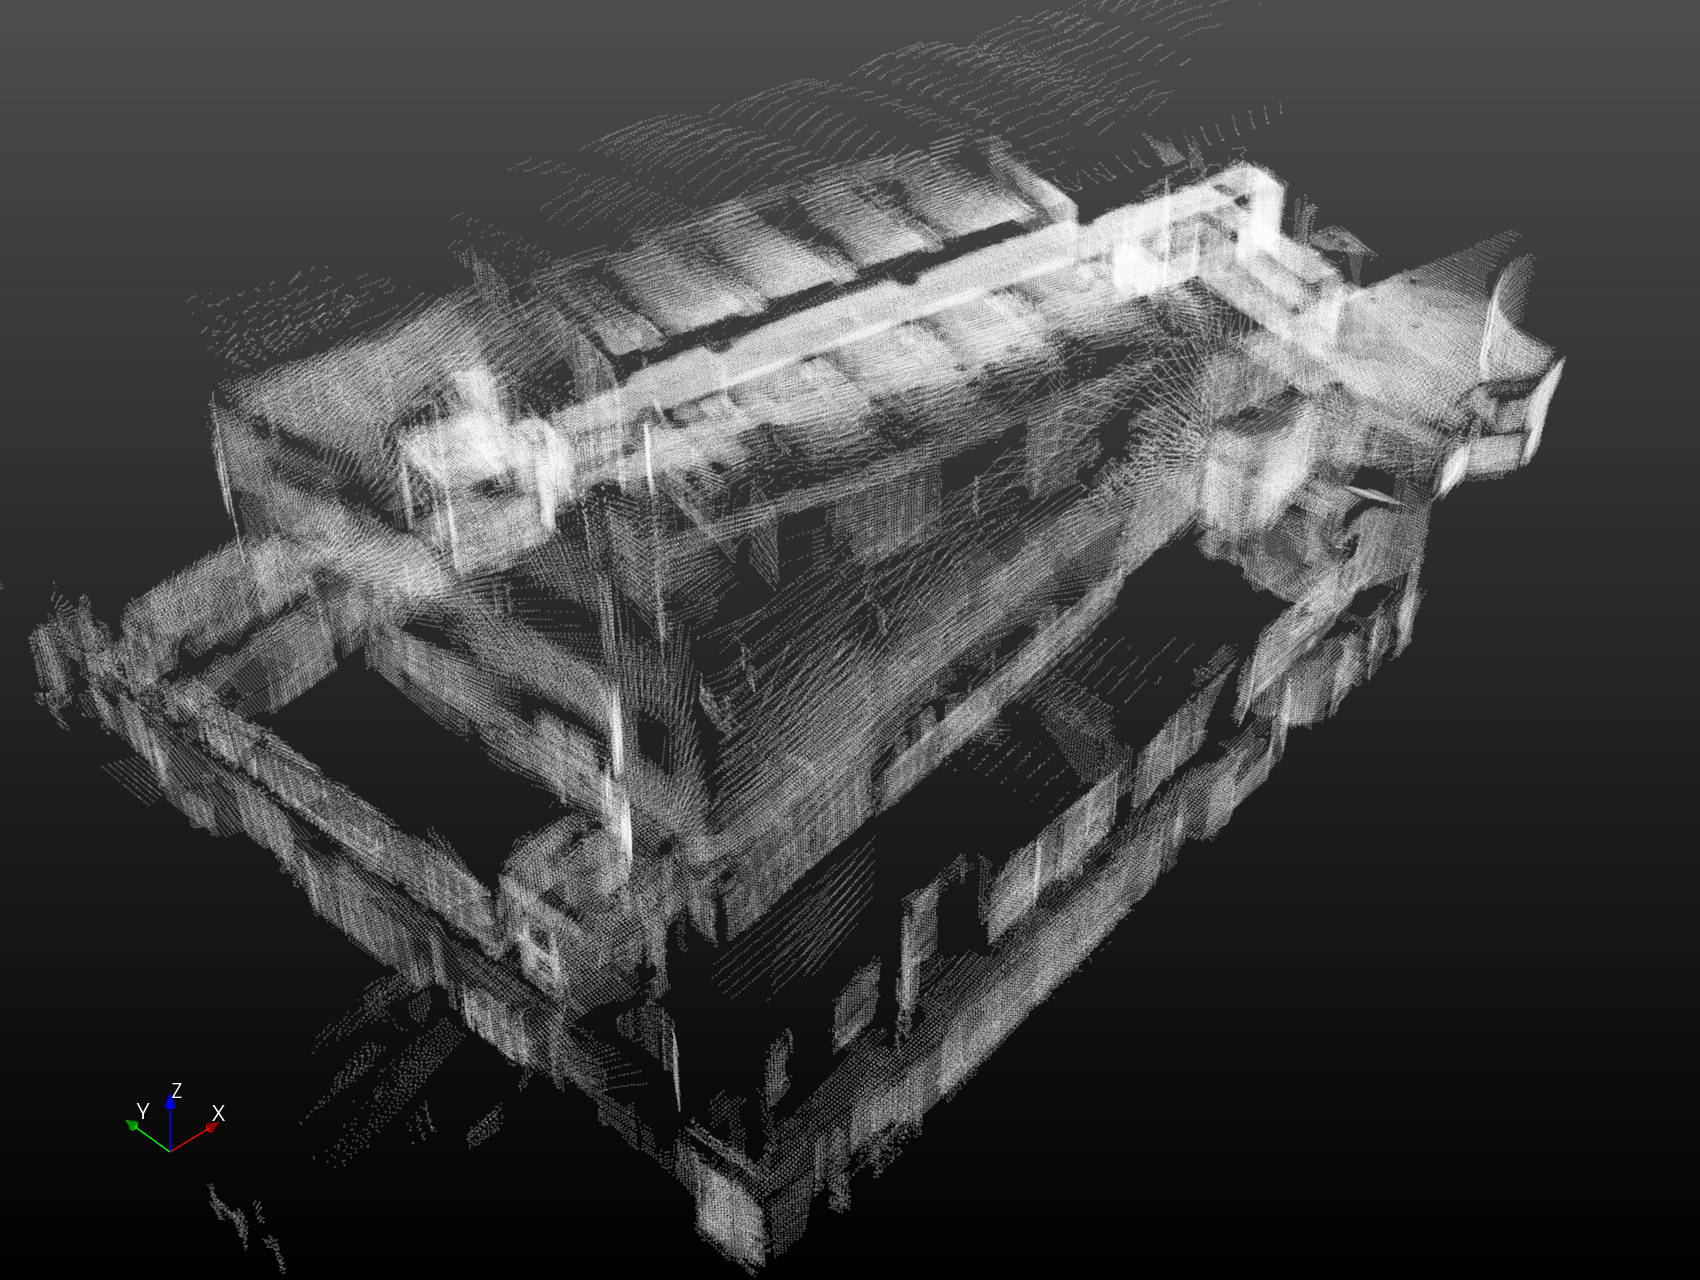
\includegraphics[width = 0.3\linewidth]{Maps2/PTCL1}} &
\subfloat{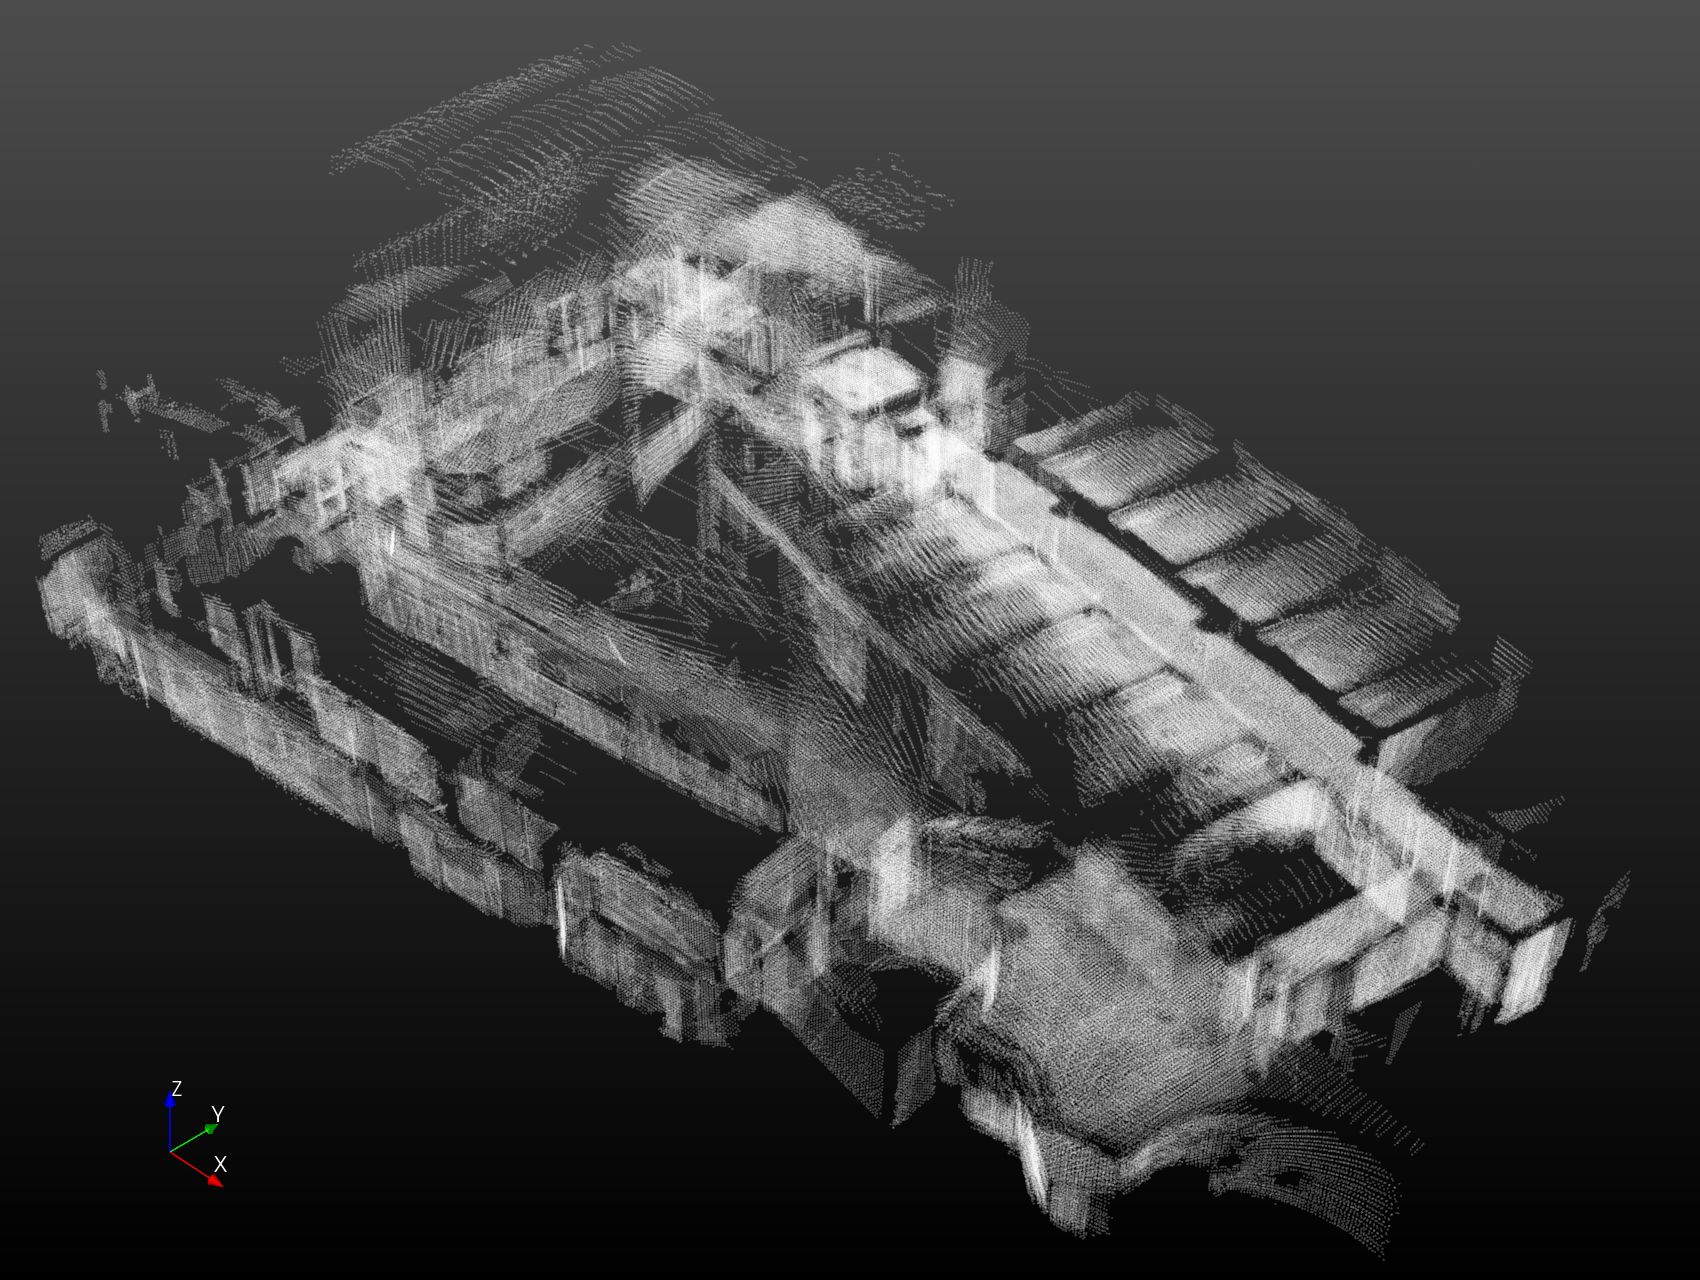
\includegraphics[width = 0.3\linewidth]{Maps2/PTCL2}} &
\subfloat{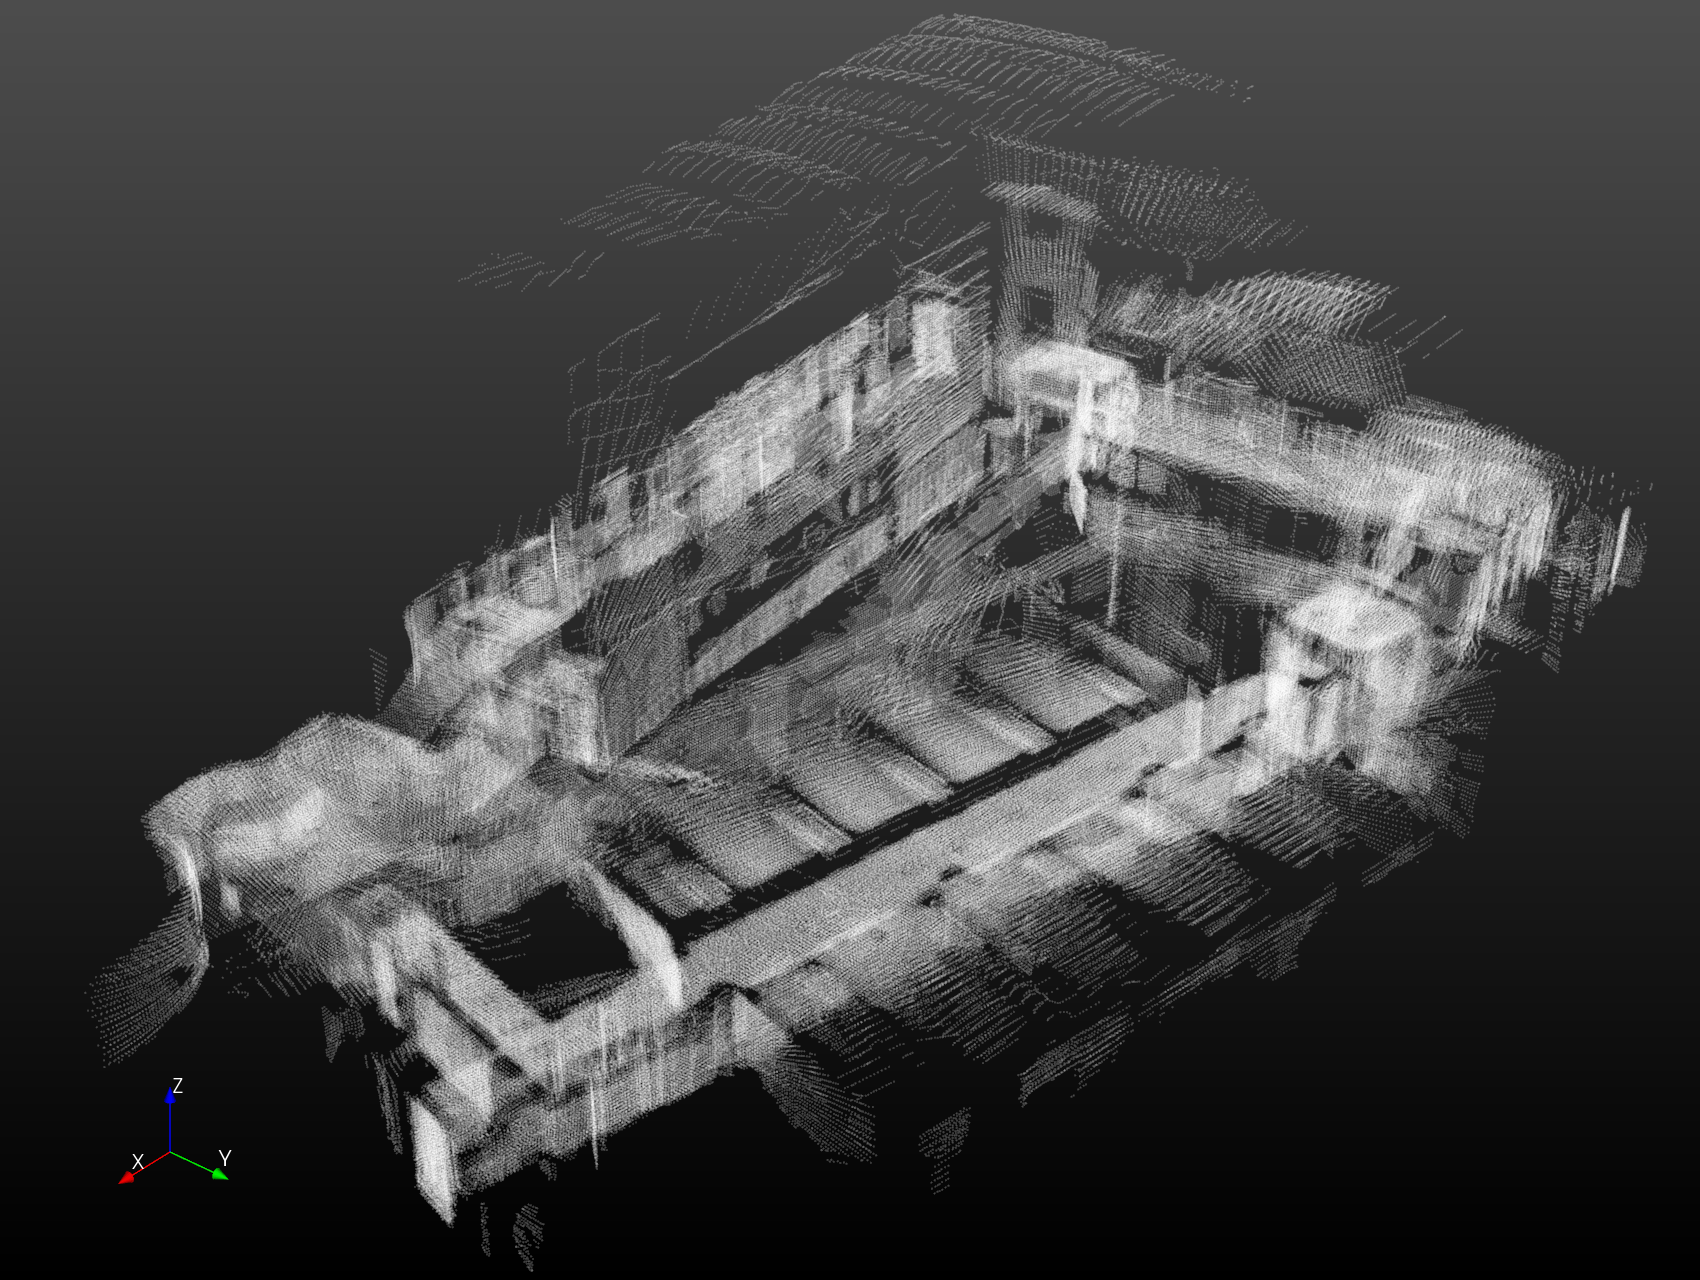
\includegraphics[width = 0.3\linewidth]{Maps2/PTCL3}} \\
\subfloat{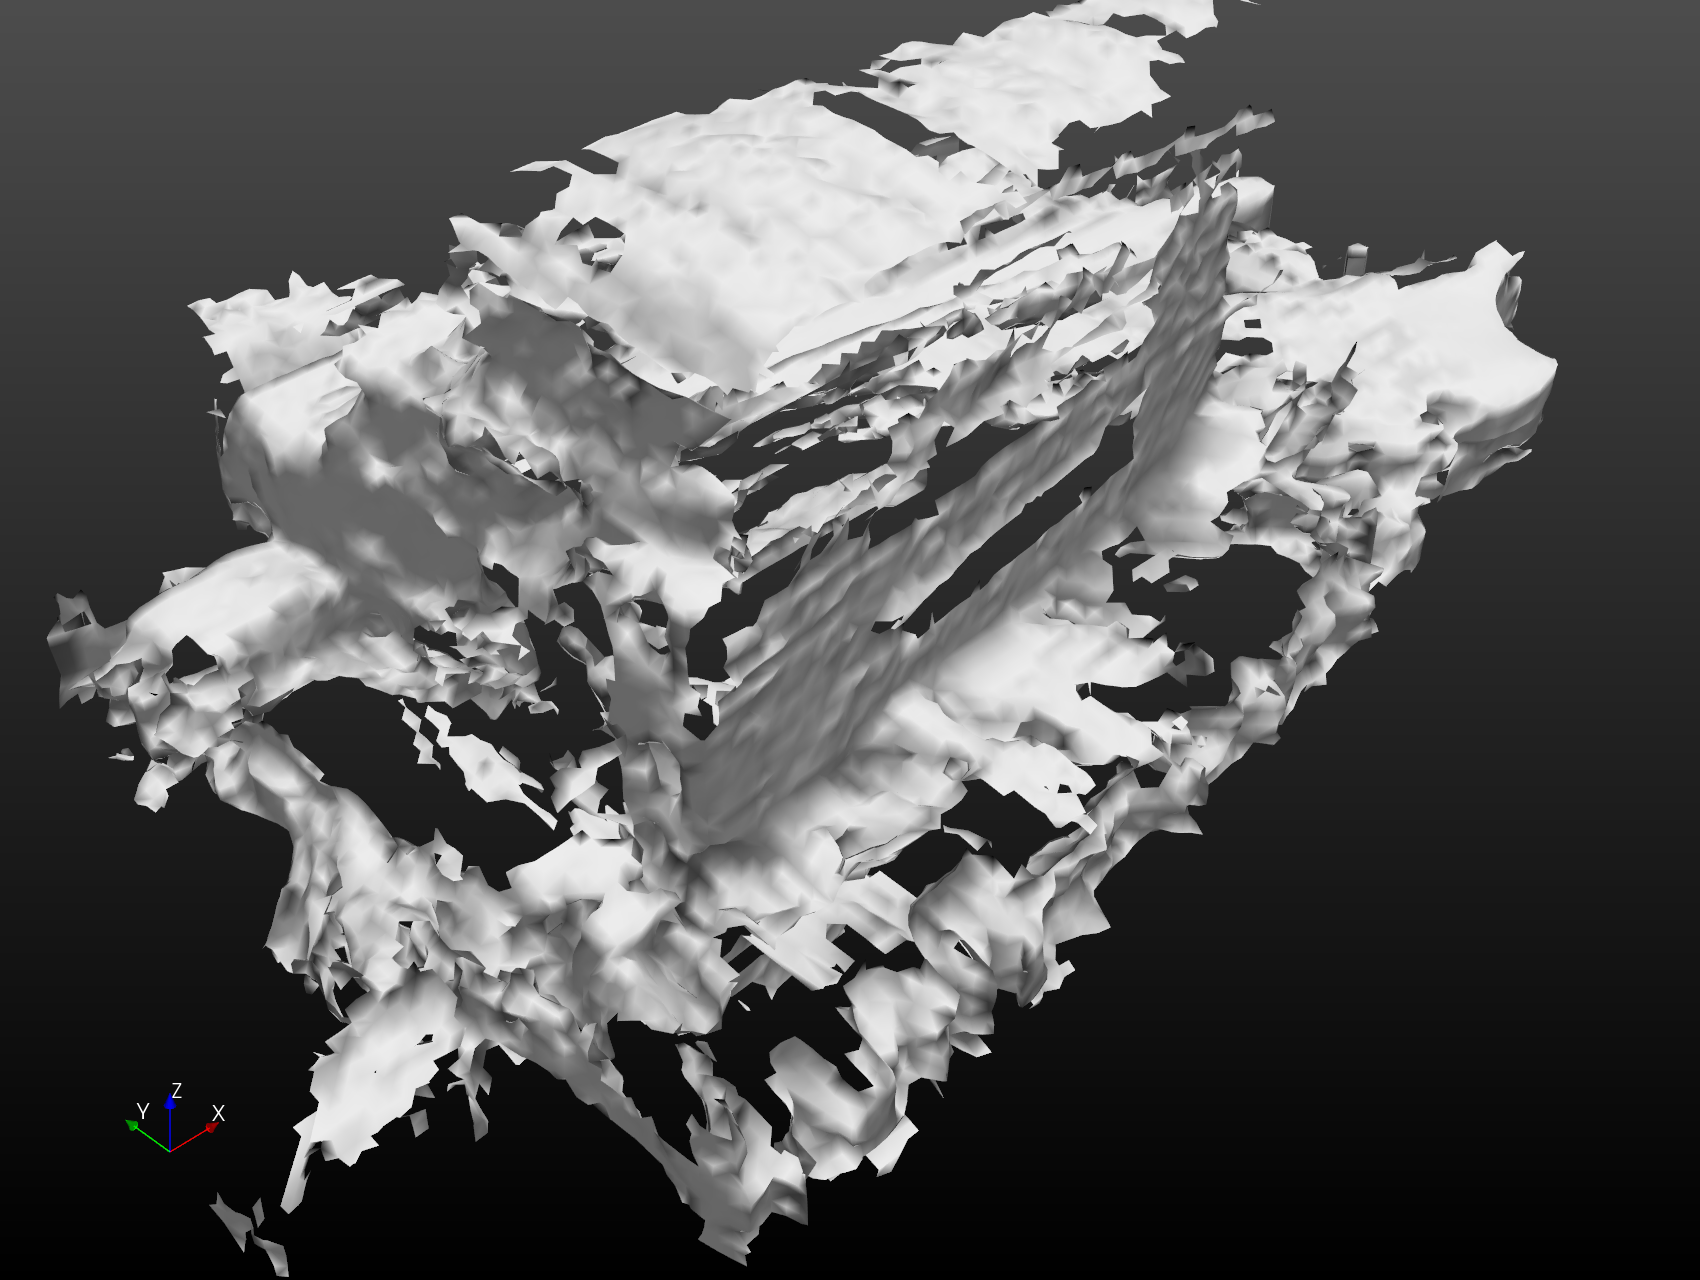
\includegraphics[width = 0.3\linewidth]{Maps2/Rec1}} &
\subfloat{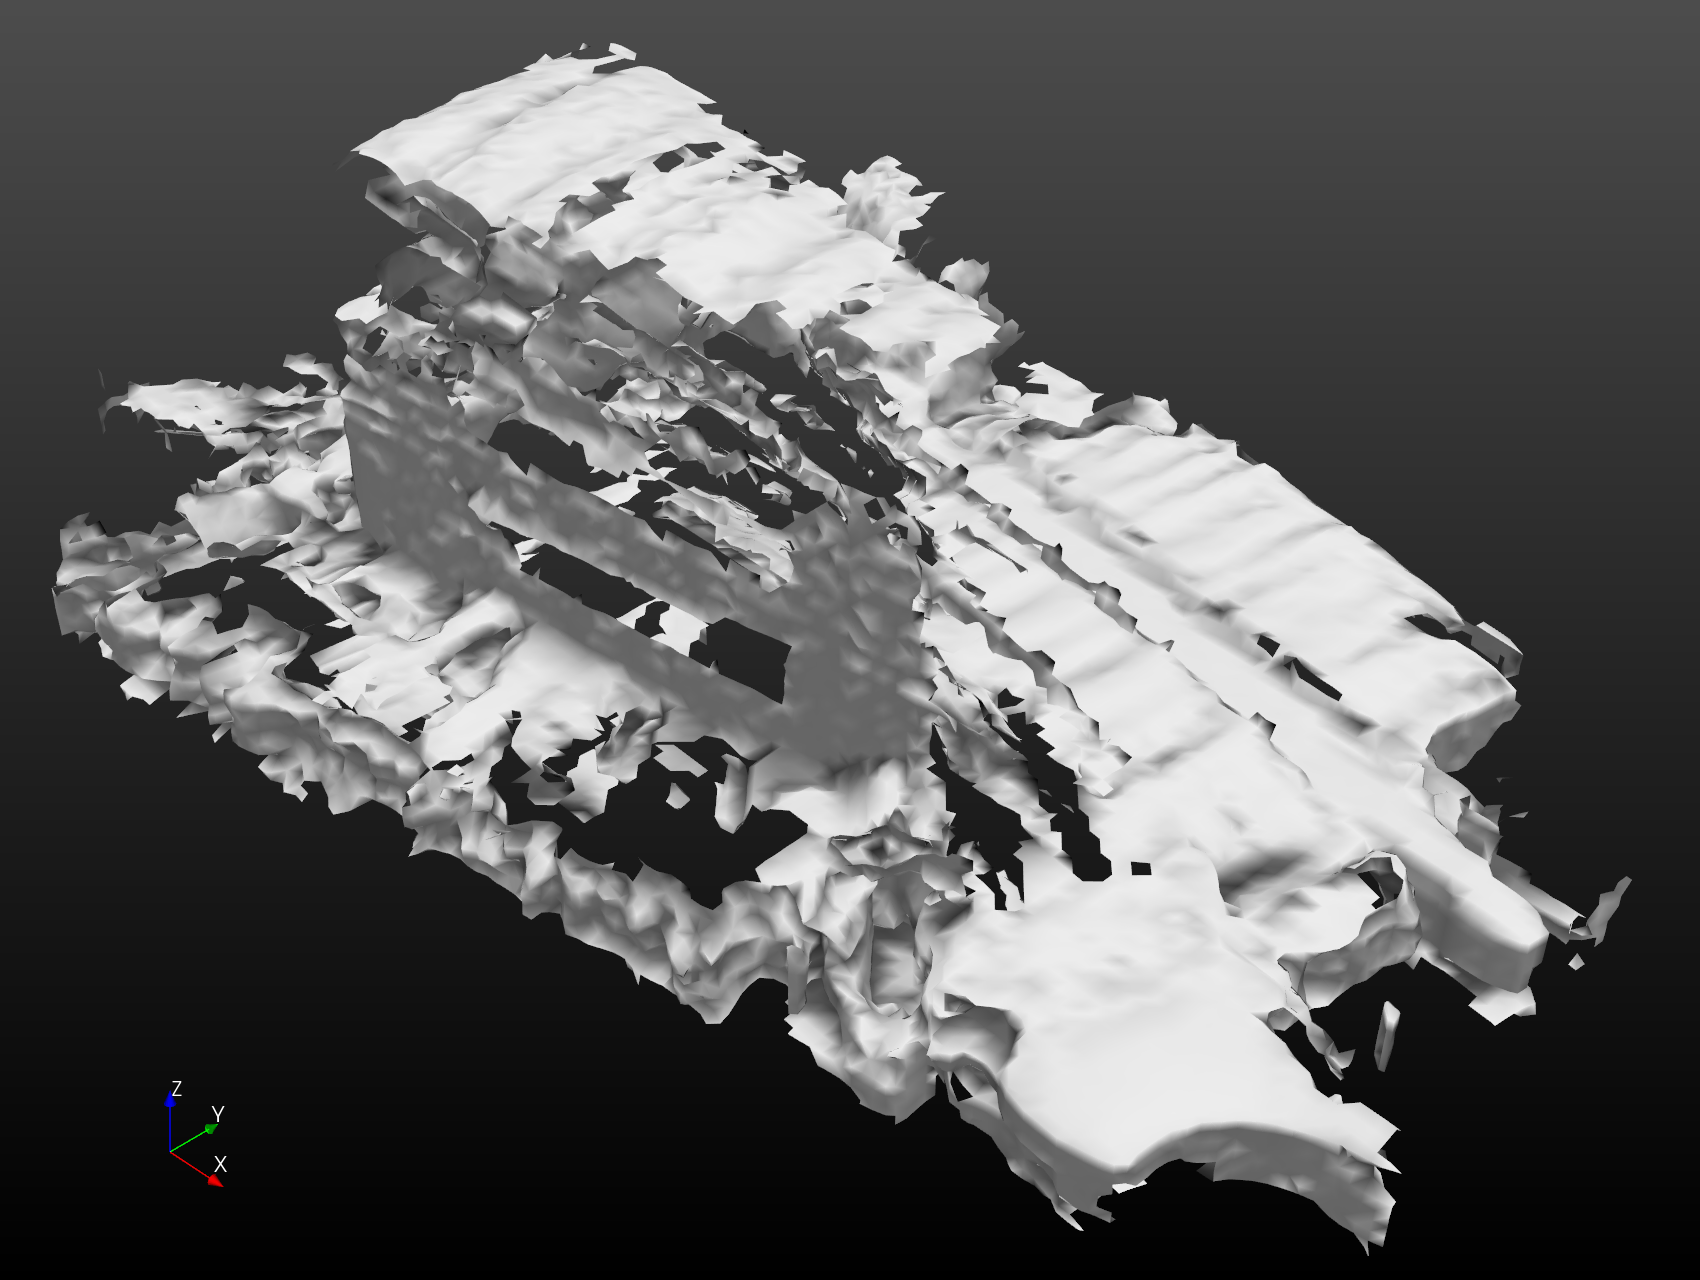
\includegraphics[width = 0.3\linewidth]{Maps2/Rec2}} &
\subfloat{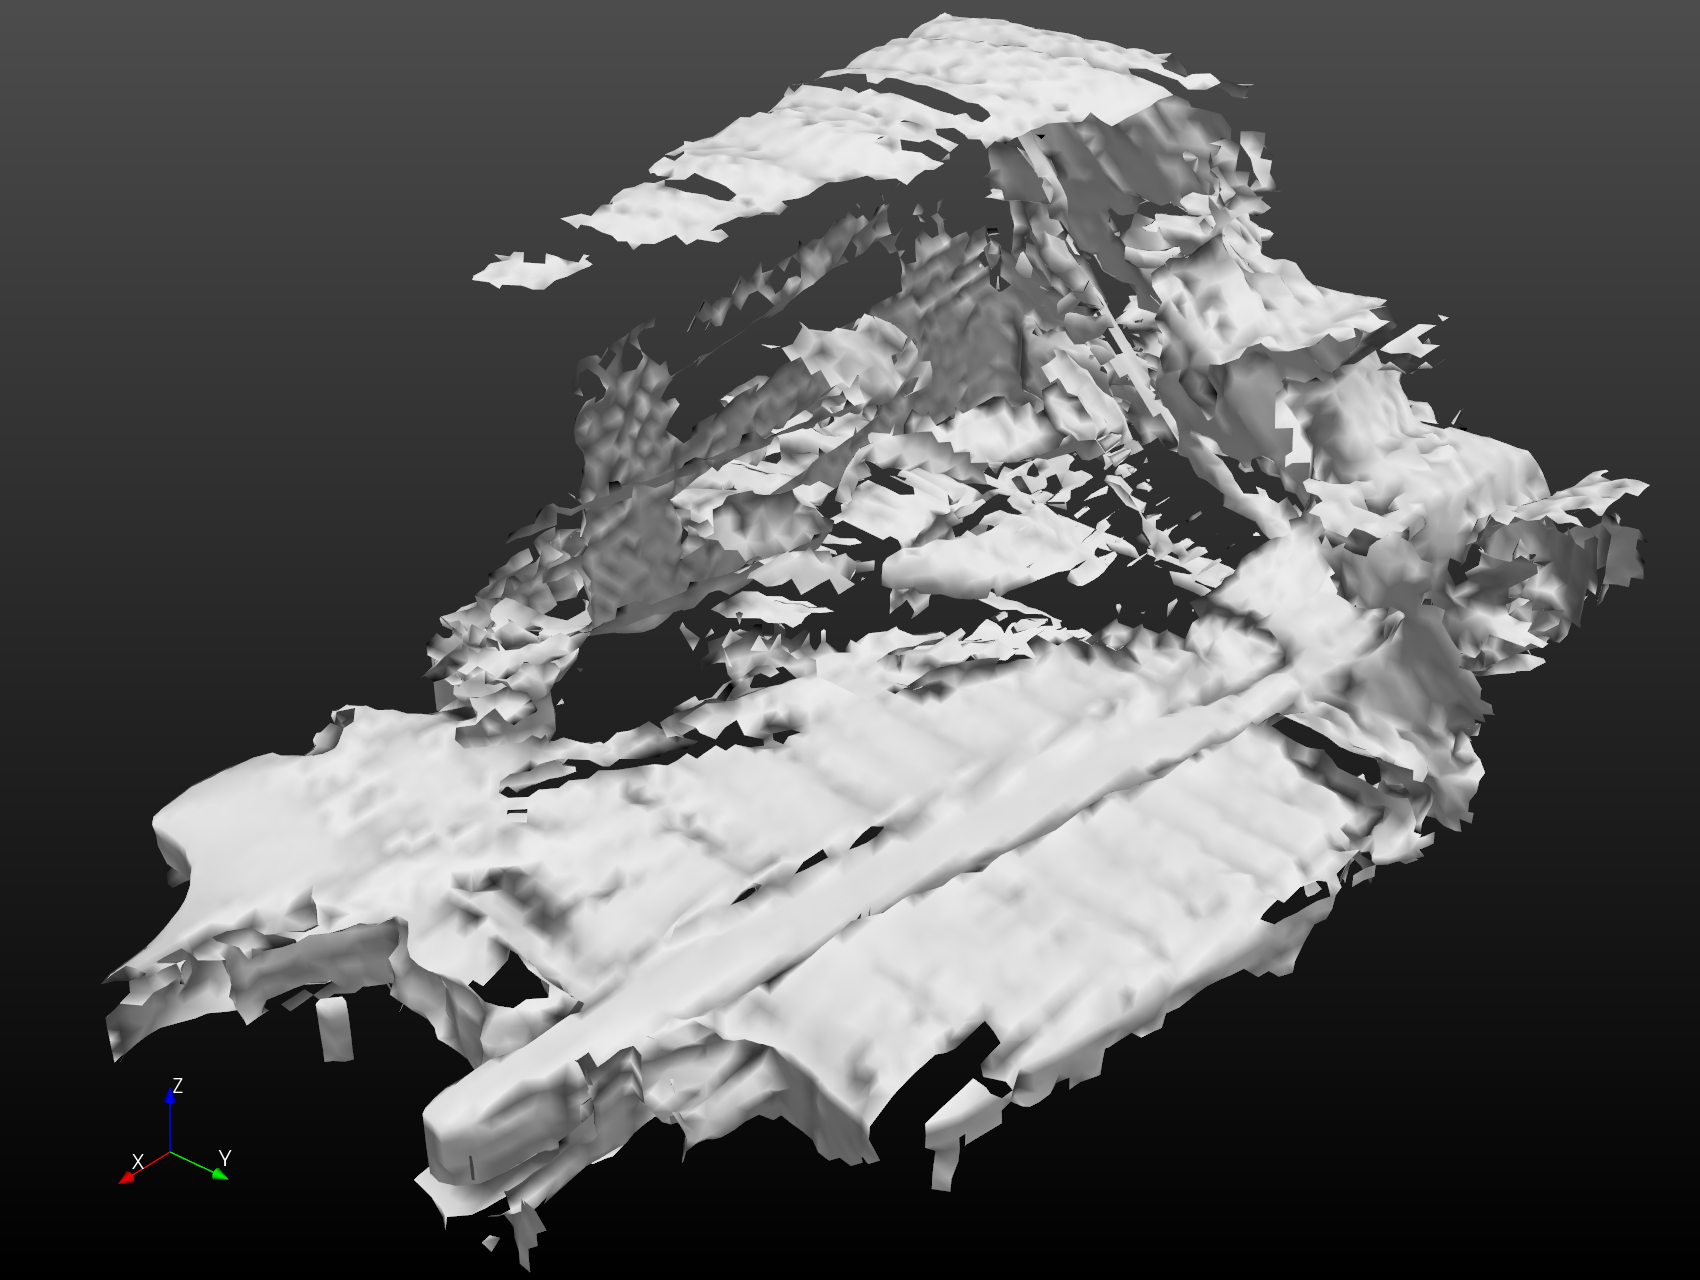
\includegraphics[width = 0.3\linewidth]{Maps2/Rec3}} \\
\subfloat{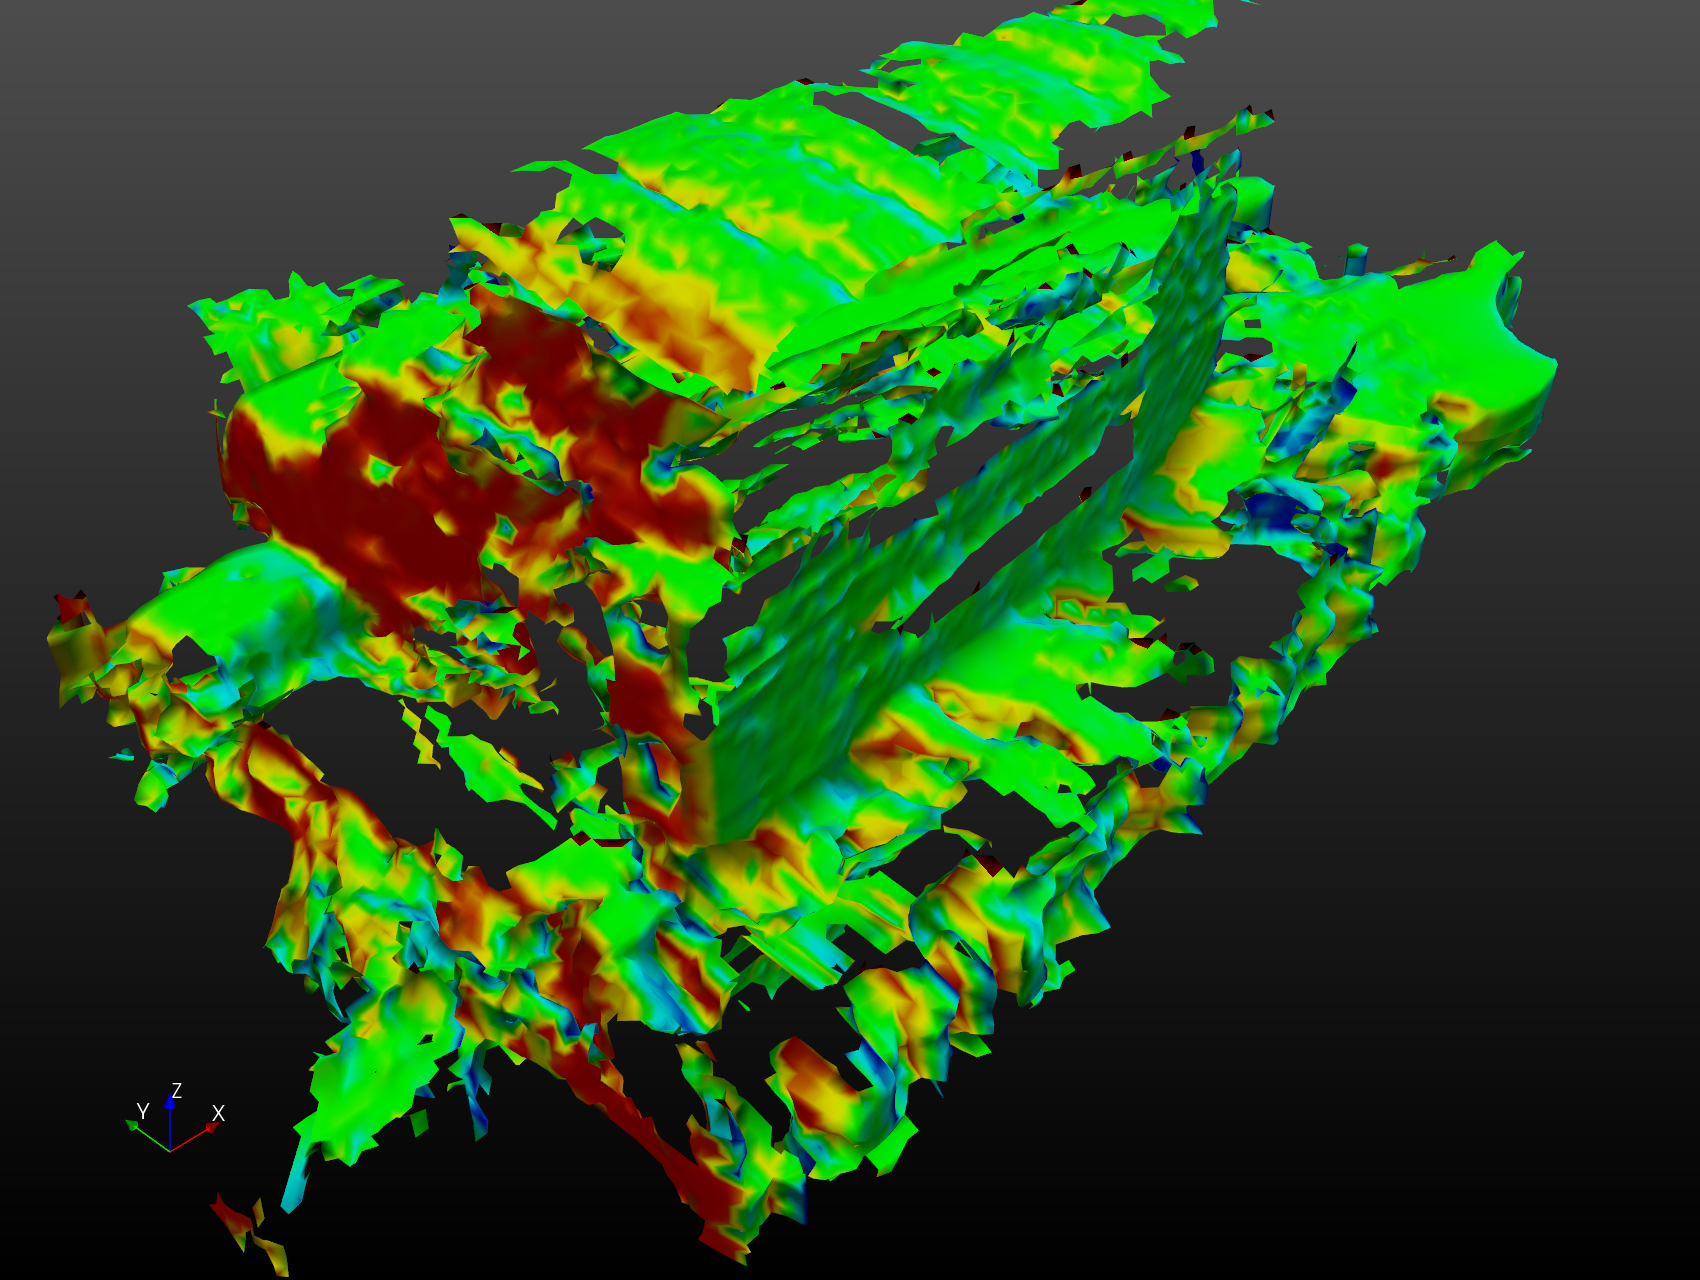
\includegraphics[width = 0.3\linewidth]{Maps2/Rec1N}} &
\subfloat{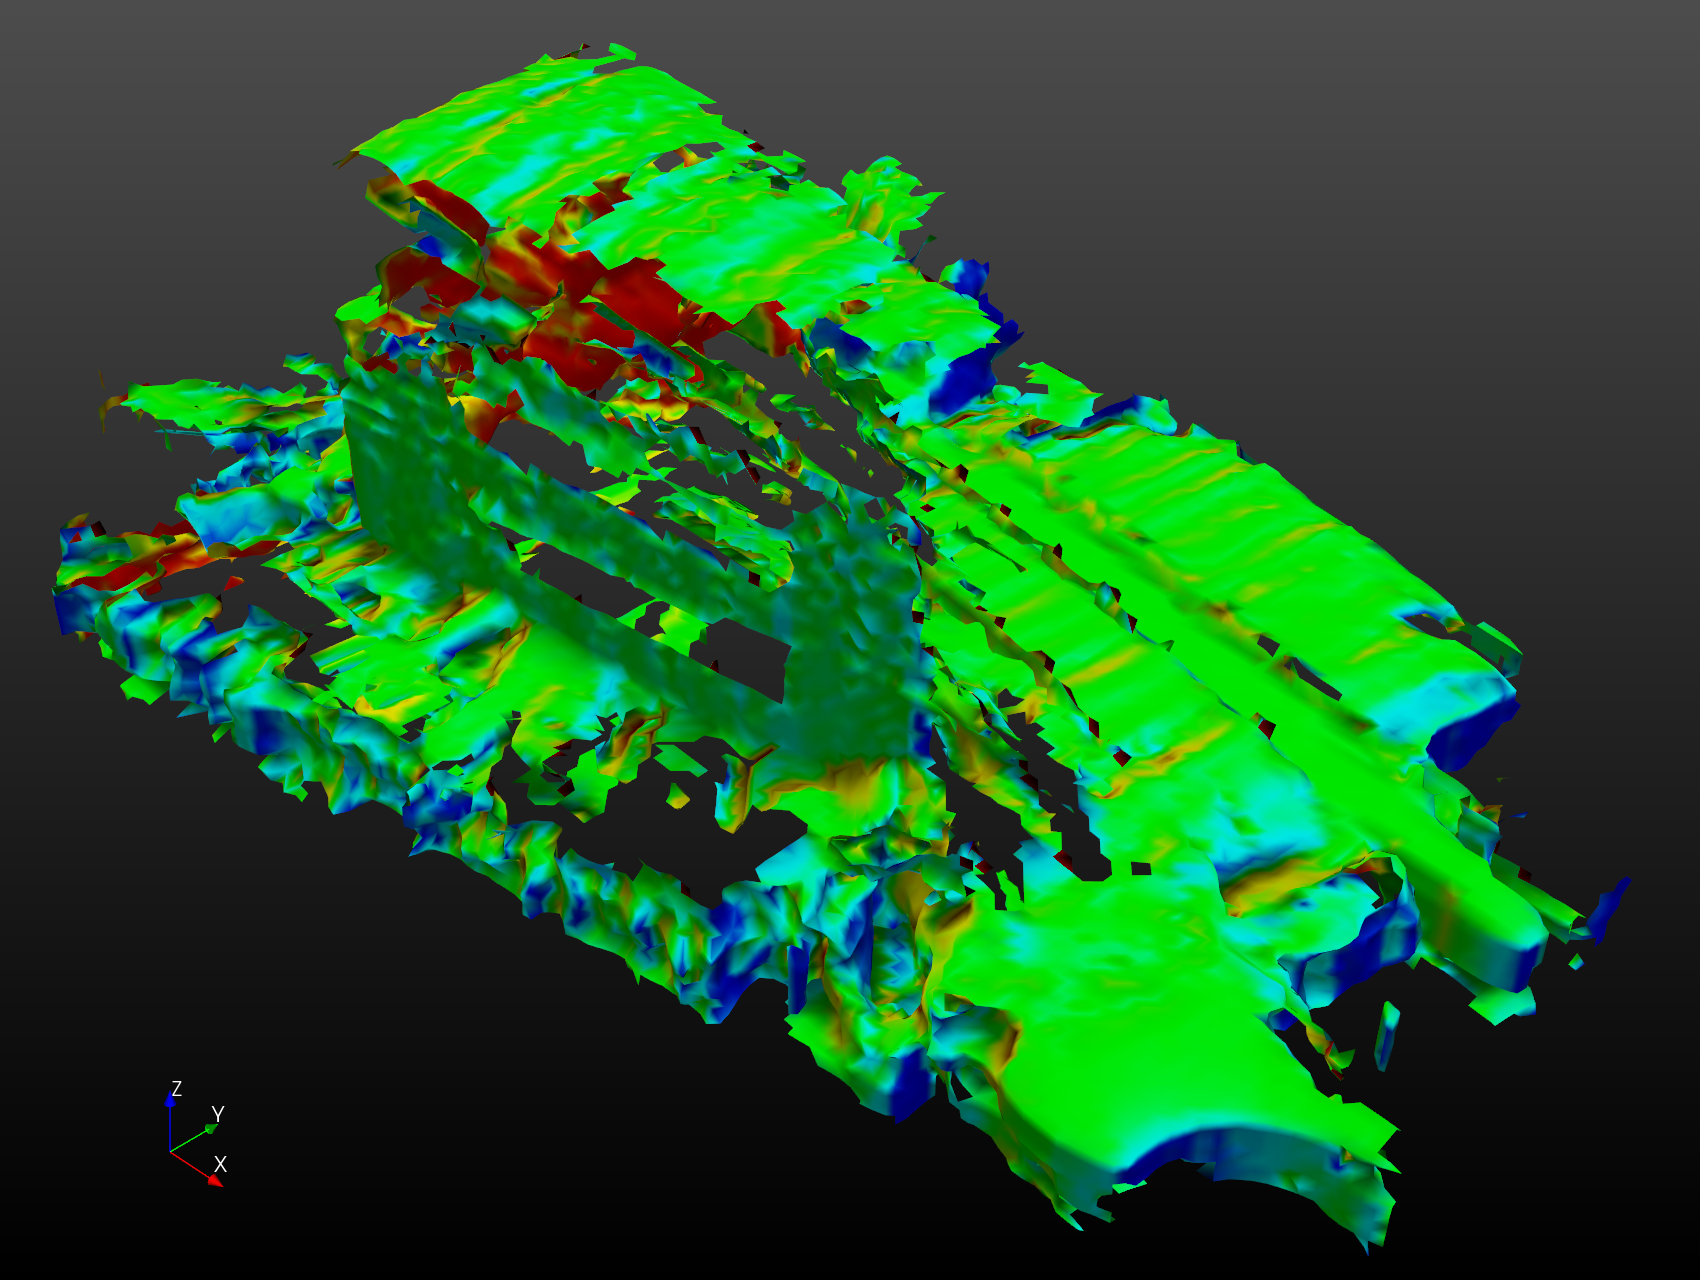
\includegraphics[width = 0.3\linewidth]{Maps2/Rec2N}} &
\subfloat{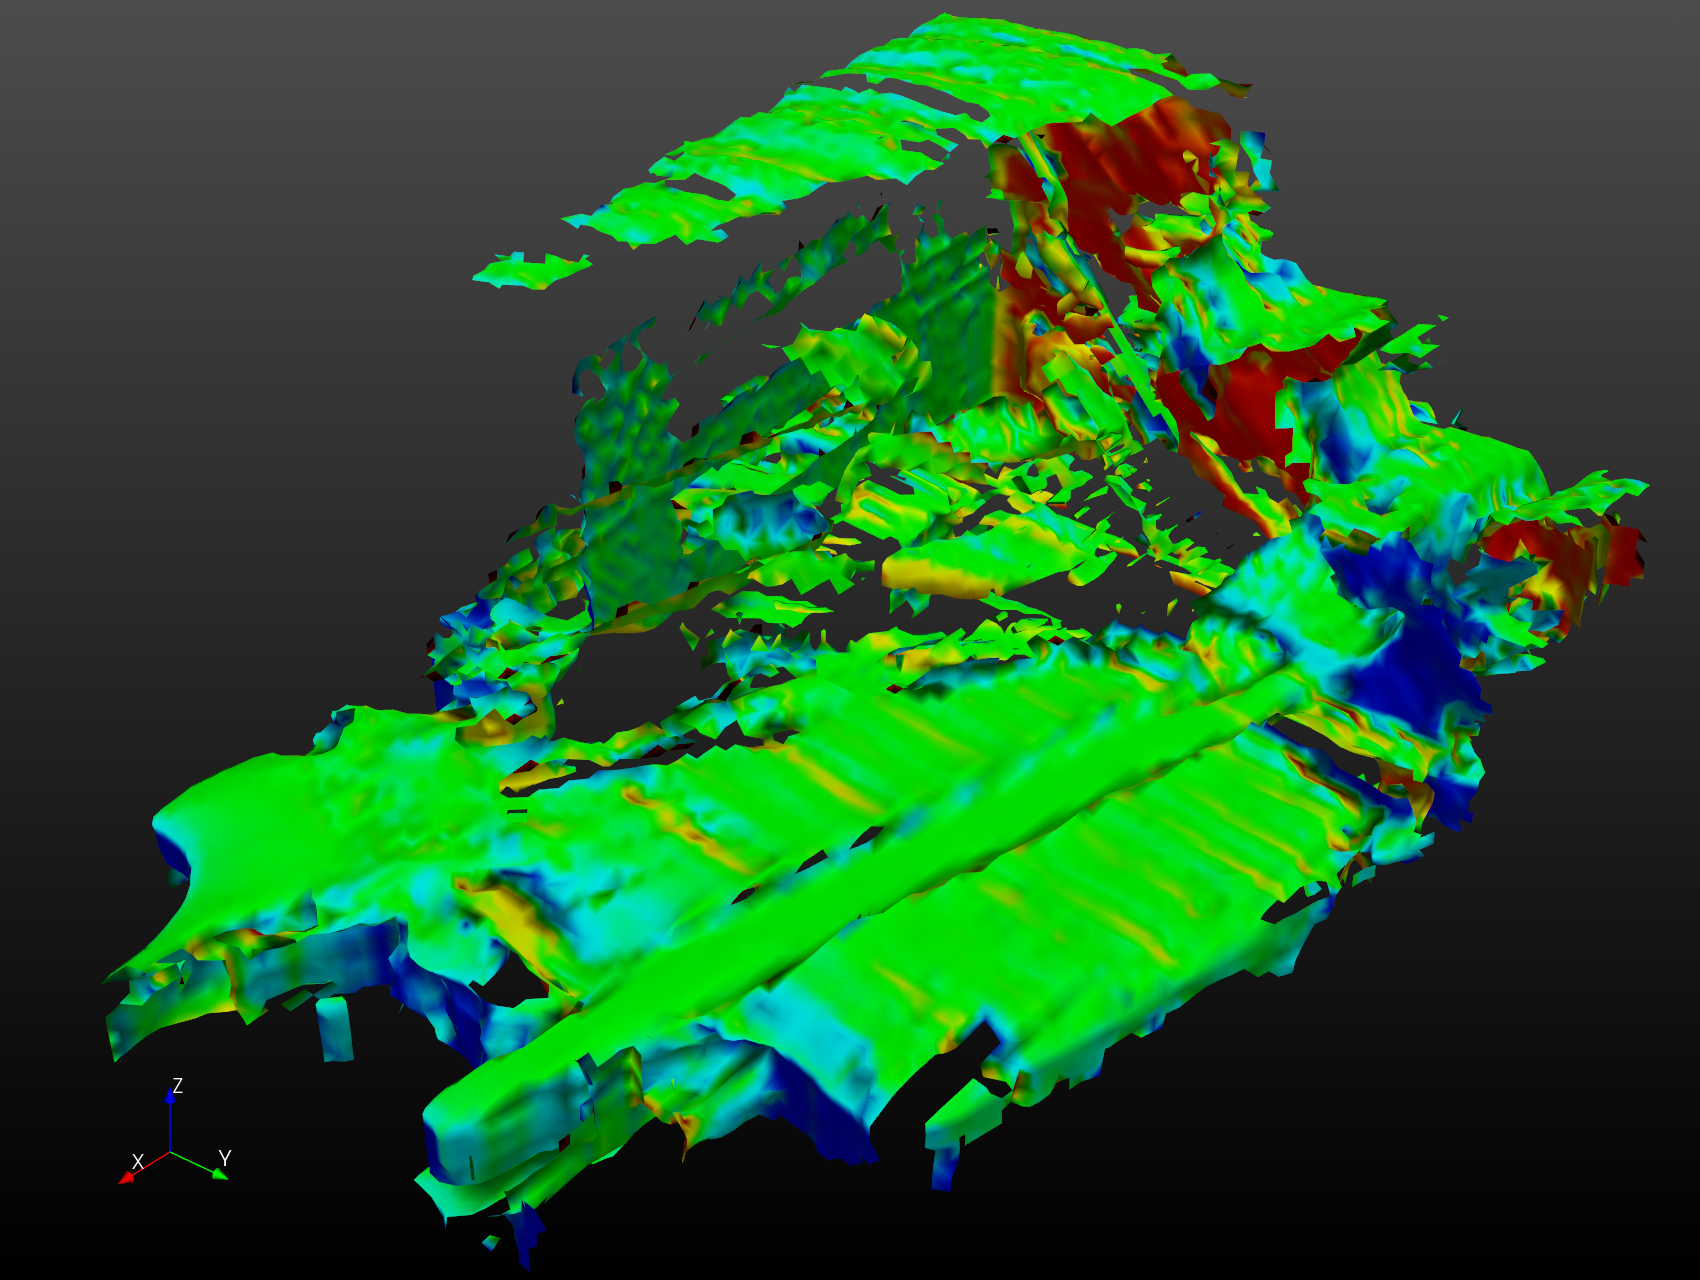
\includegraphics[width = 0.3\linewidth]{Maps2/Rec3N}} \\
\subfloat{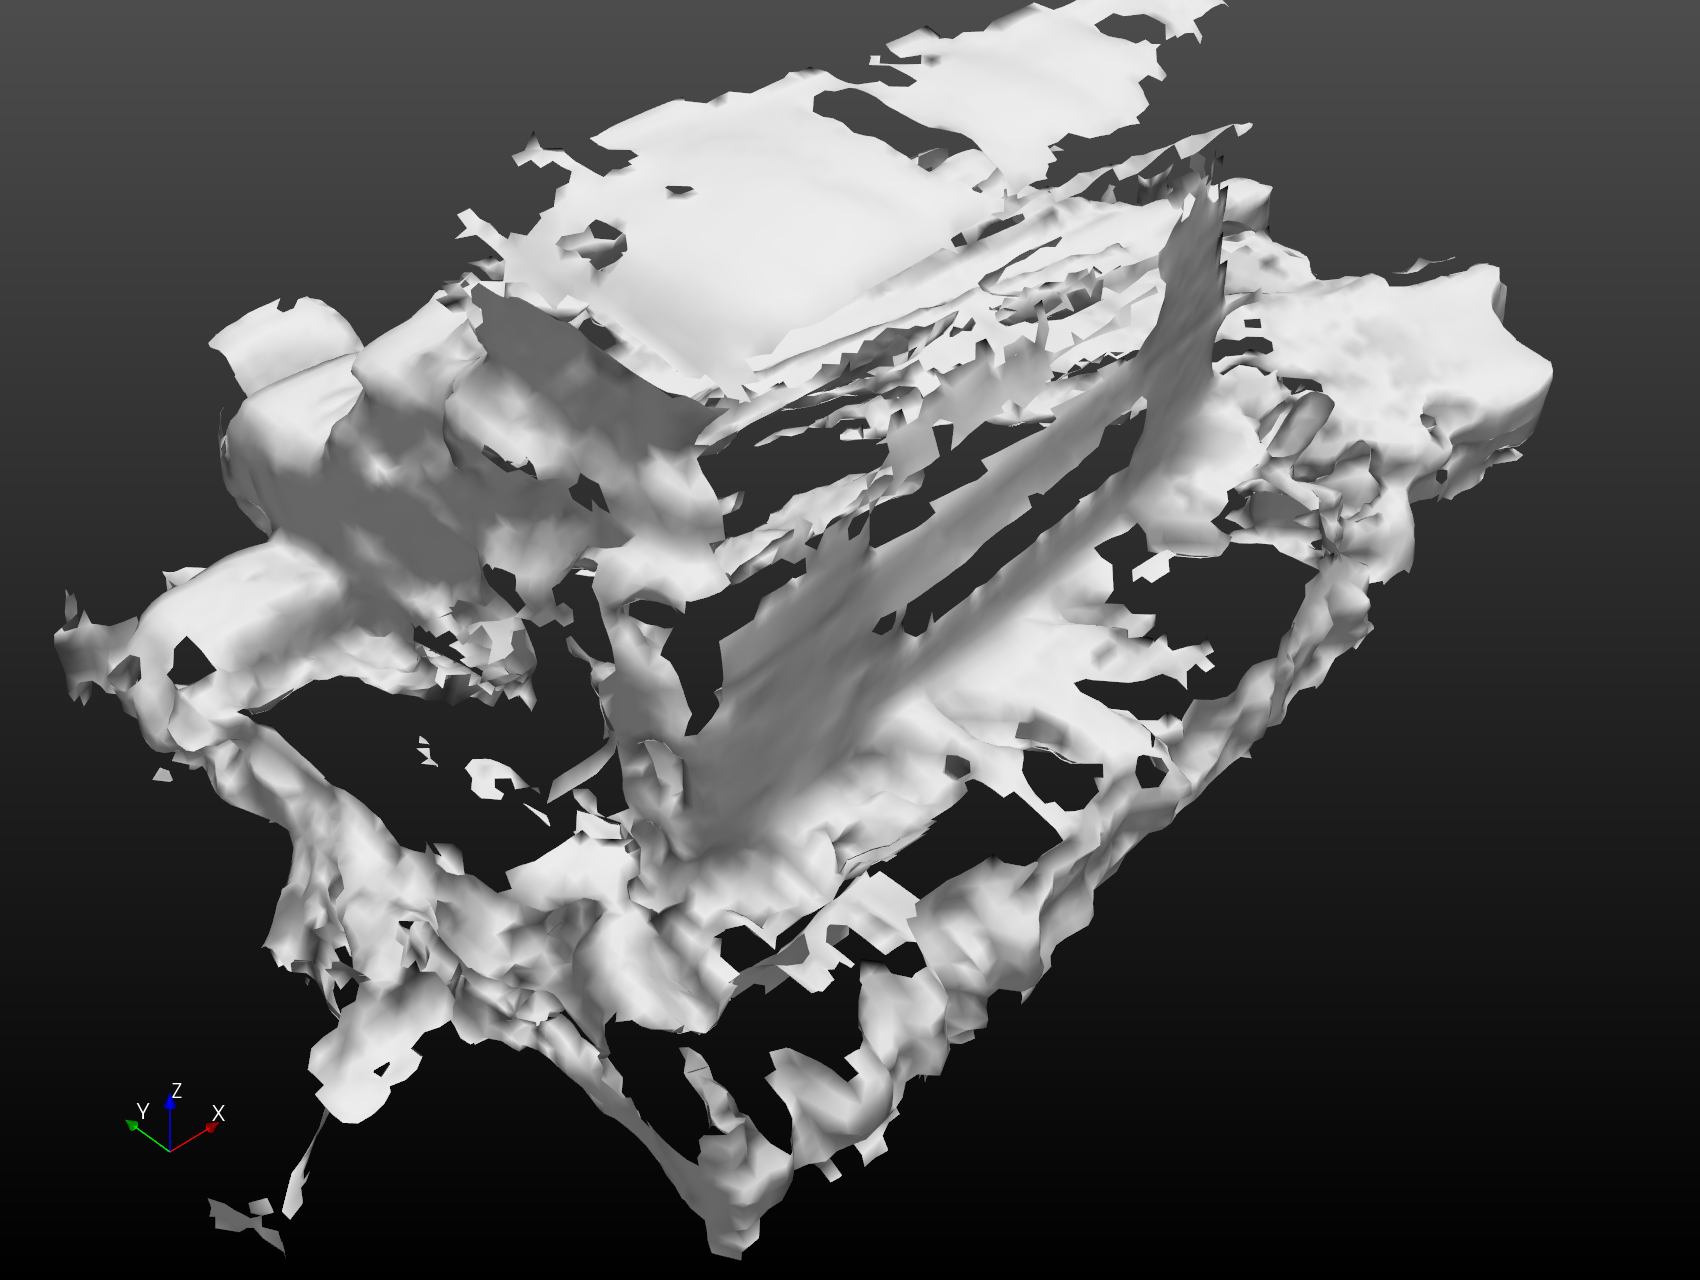
\includegraphics[width = 0.3\linewidth]{Maps2/RegRec1}} &
\subfloat{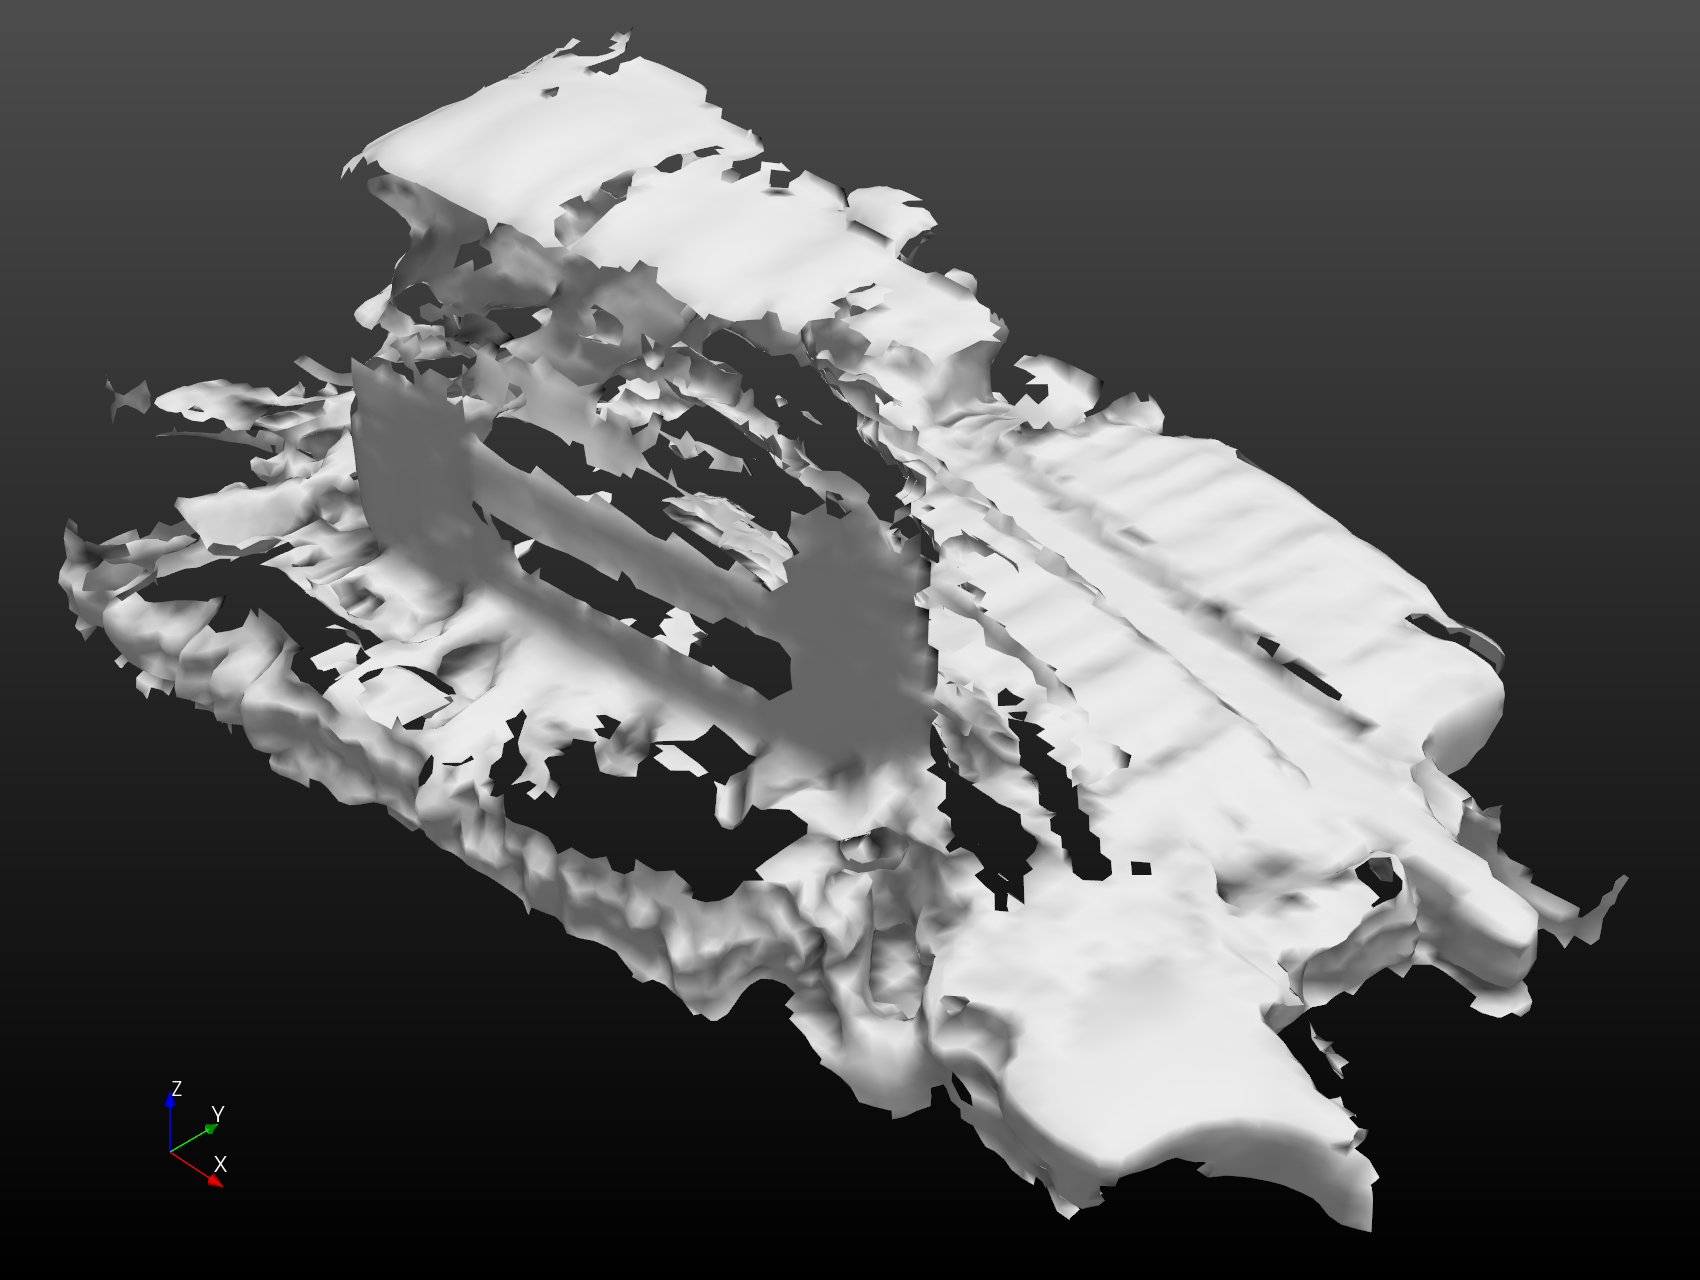
\includegraphics[width = 0.3\linewidth]{Maps2/RegRec2}} &
\subfloat{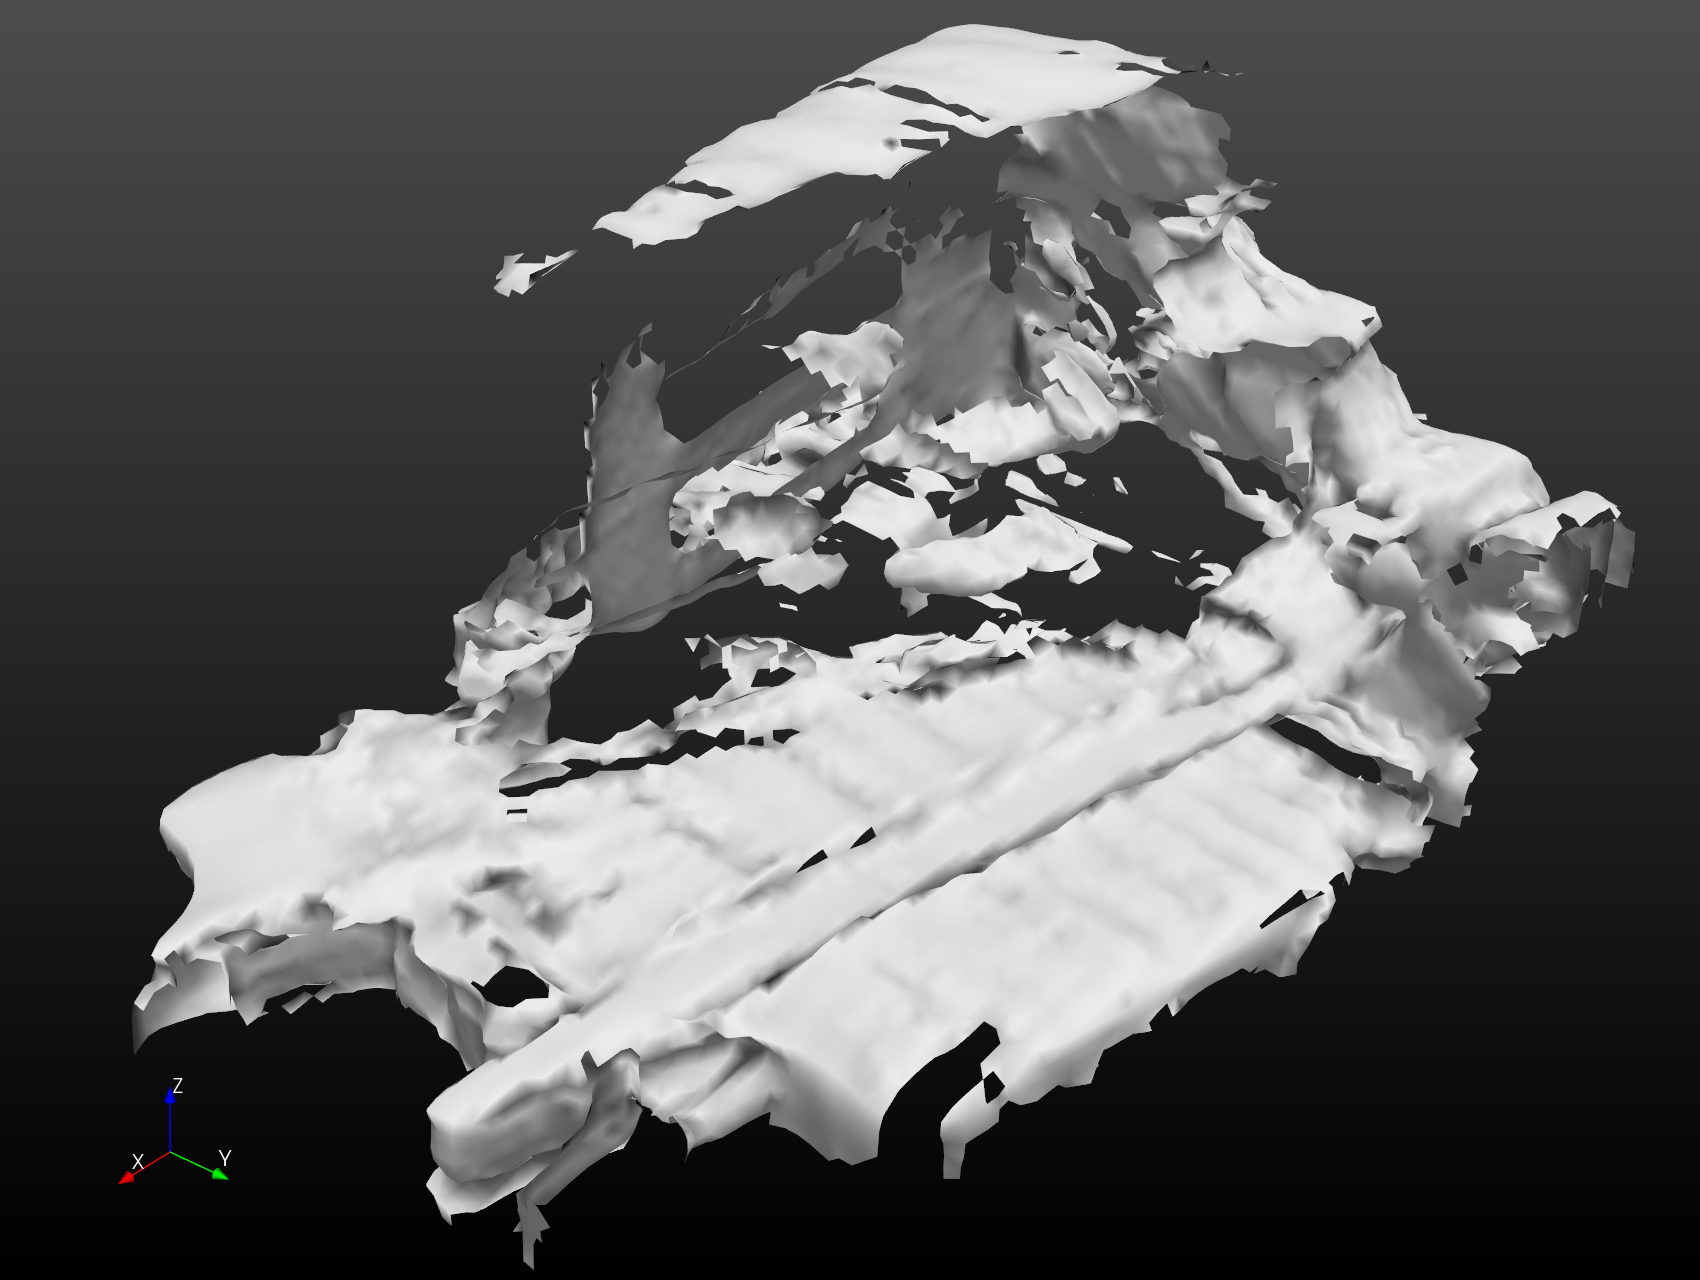
\includegraphics[width = 0.3\linewidth]{Maps2/RegRec3}}\\
\subfloat{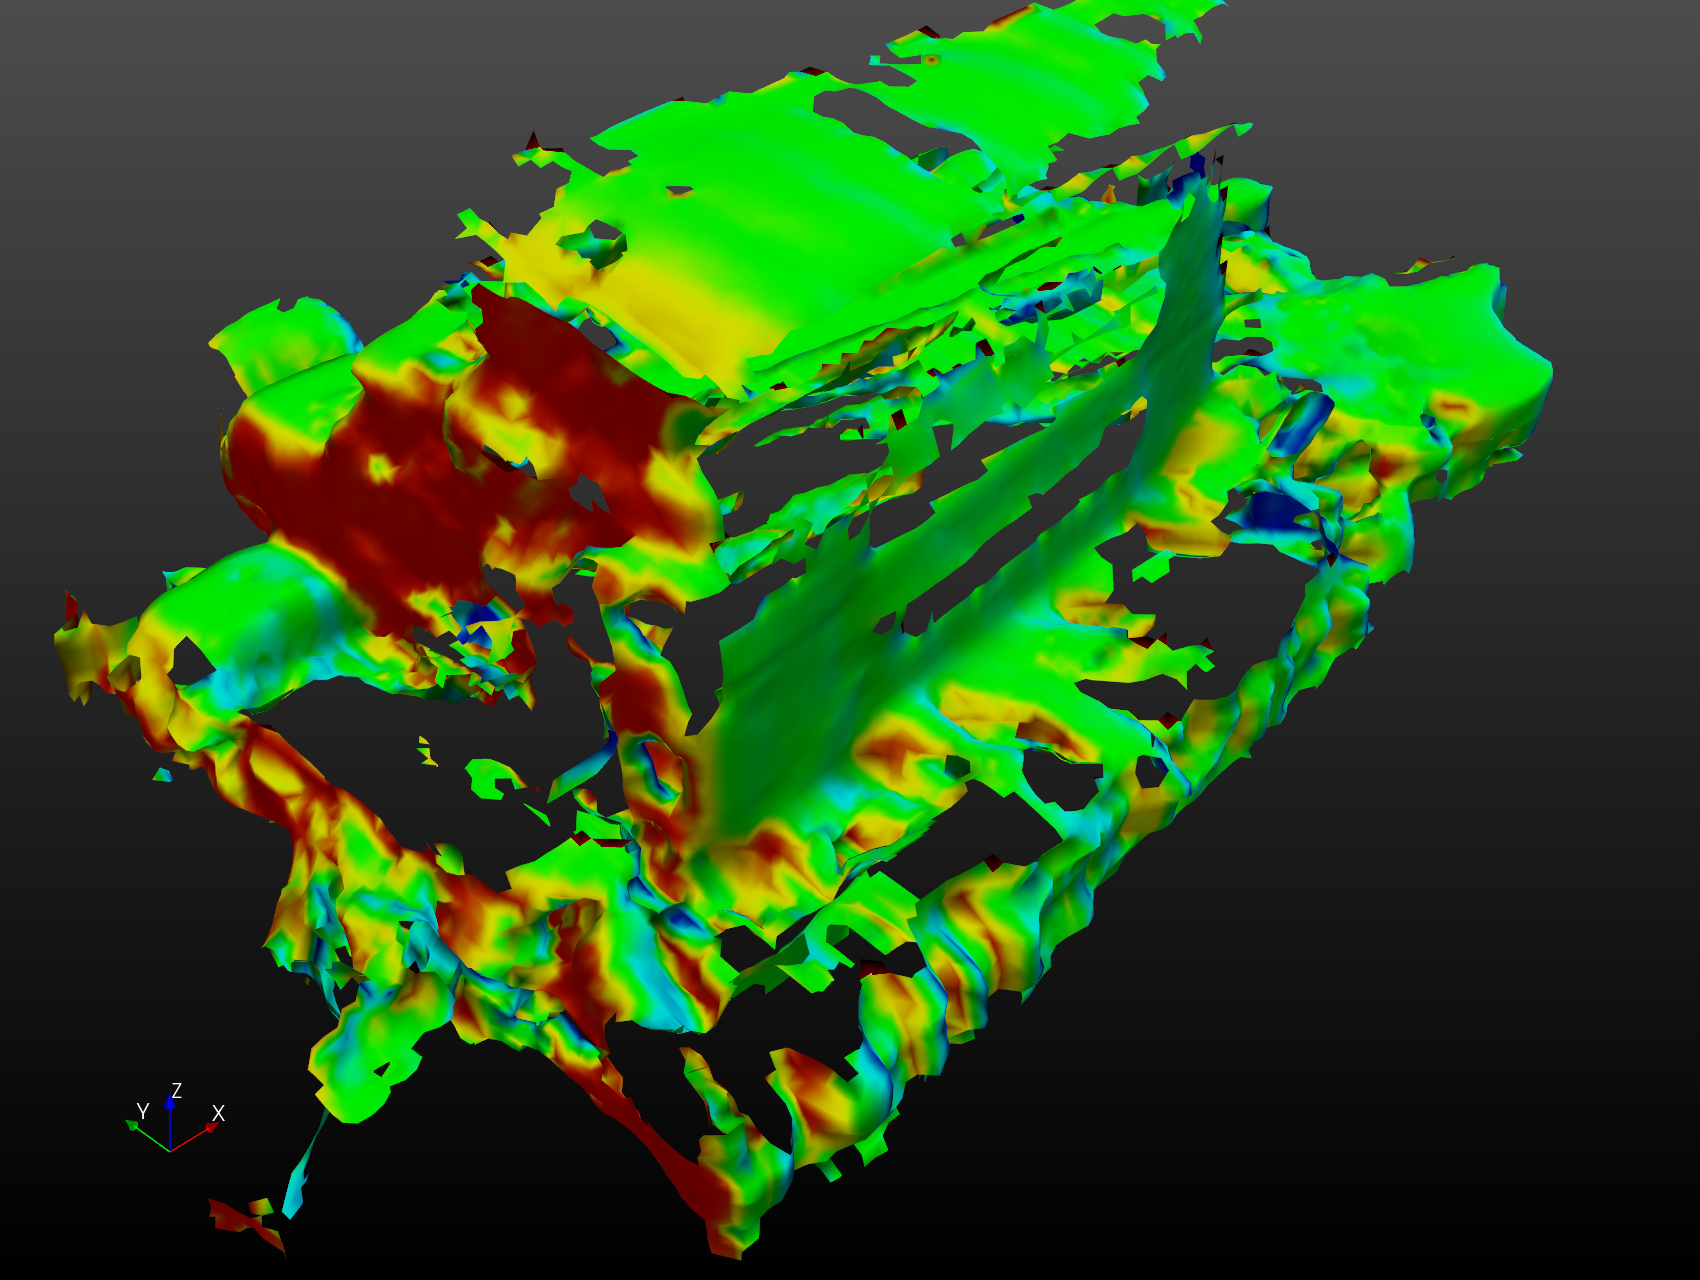
\includegraphics[width = 0.3\linewidth]{Maps2/RegRec1N}} &
\subfloat{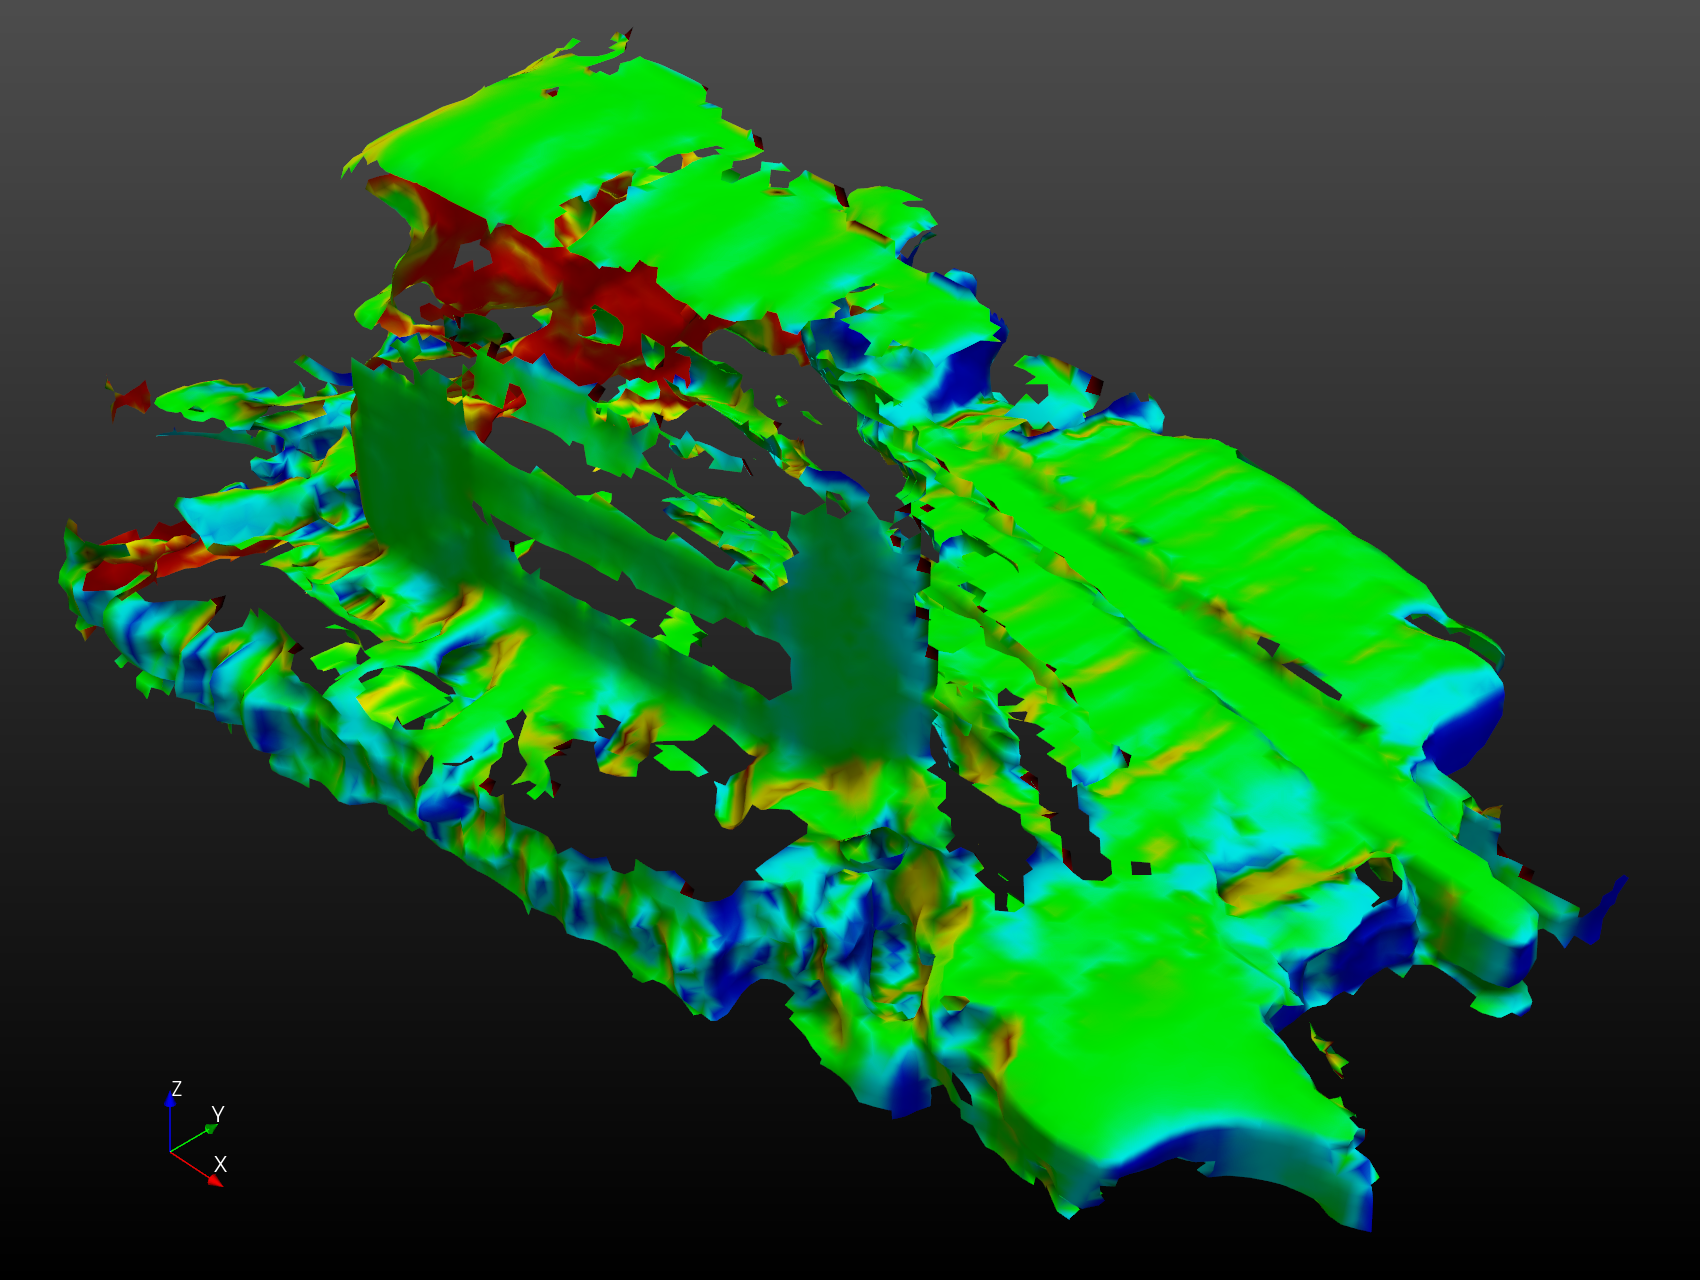
\includegraphics[width = 0.3\linewidth]{Maps2/RegRec2N}} &
\subfloat{\includegraphics[width = 0.3\linewidth]{Maps2/RegRec3N}}
\end{tabular}
\caption{Results of running BORG CUBES to point clouds from first row. Second and third rows shows unregularized reconstruction (solid and normals coloured). Fourth and fifth rows show regularized reconstructions with $\lambda$ = 0.1 and 50 iterations (solid and normals coloured).}
\label{fig:IEBDataset}
\end{figure}	
	
The second and third rows show the reconstruction without any regularization. Since the point clouds were sparser here, different parameters were used. The voxel edge length was set to 0.3m and the fusion threshold was set to 8. Noticeably, the corridor in the first picture from left to right of the second row got its walls merged. That is because this corridor is narrow, and the increase in the voxel edge length and the fusion threshold cause points in different walls to be merged together. A decrease in either of those two parameters would mean less surfaces being reconstructed though. So there is a trade-off when narrow spaces are concerned.
	
The fourth and fifth rows show the reconstruction using a $\lambda$ of 0.1 and 50 iterations. It is noticed that the surfaces got smoother than the original reconstruction, and again some surfaces were removed as they were interpreted as noise by the algorithm.

	\subsection{Final Evaluation}
	
In general, the two maps above have many holes in the final reconstruction. Those are due to the lack of LiDAR points in certain areas. When applying this pipeline to real-life applications, many strategies can be taken to overcome this problem. To cite a few: (i) Many LiDAR sensors could be used instead of just one; (ii) The robot could move slower to map the entire building and get denser representations of the environment; (iii) Other sensors could be embedded, such as visual and depth sensors.
	
As explained in the last section, the parameters for the reconstruction can be arbitrarily set based on limitations on the hardware or specific applications for the whole pipeline. The ones chosen at the experiments were set with the intention of providing the best visual representation of the performance of the algorithm.
		
	\newpage
	\section{Conclusion}
	
In this project, it was shown a setup that solves the SLAM problem and reconstructs a large-scale indoor environment using LiDAR data. The system can be implemented in real time and incrementally, since all of the algorithms used are incremental solutions.
		
In such a broad and big problem, there are a couple of issues in the system that needs to be addressed in subsequent projects:
	
\paragraph{Loop Closure: } The loop closure system as implemented is simple enough for small drifts in a structured environment. However, it is very sensitive to changes in the parameters. As it was shown in Section \ref{subs:LoopCl}, different parameters yield significantly different maps, which is not good for a robust and embedded solution. Also, this solution does not take into account larger drifts. If a mobile robot does not perform loop closures in a relatively small amount of time, it might drift so much that the heuristics used (especially the Euclidean Distance) would remove this possible closure immediately. Other solutions taking into account visual cues (as extensively described in the literature) would have to be implemented to take those into account.
	
\paragraph{Multihypothesis: } Related to the Loop Closure problem, it is needed a robust solution to prevent wrong loop closures from happening. Regardless of how the loop closure system is implemented, it will make mistakes, and those can be catastrophic to the final map. A robust solution then is necessary to avoid that small perturbations in the loop closing problem lead to totally erroneous maps being created.
	
\paragraph{3D Reconstruction: } In this report, RGB or depth images were not used in the 3D reconstruction. As explained in Section \ref{sec:Borg}, this is because RGB data are less effective for long distances and depth images are not suitable for outdoors applications. However, without RGB data, a sparse map is generated, since only LiDAR data is available for the 3D reconstruction. Since Borg uses sensor-agnostic voxels, it would be convenient to try a denser data generation, which would result in better maps.
	
\paragraph{Outdoors Experiments: } It would also be beneficial to test this system in a dataset that is mainly outdoors. None of the sensors used are not suited for outdoors applications, so the system should perform as expected. However, real life validation would have to be taken to agree with the theoretical grounds.


		
	\newpage
	\bibliography{4YPReportBibl}
	\bibliographystyle{ieeetr}

\end{document}
